% Note: arara is like “make” for latex. Run with “arara main”.
% arara: pdflatex: { draft: true }
% arara: biber
% arara: makeindex: { style: main.ist }
% arara: pdflatex: { synctex: true }
% arara: pdflatex: { synctex: true }
\documentclass[11pt, a4paper,onecolumn, twoside,french]{report}
% openany -> for drafts
\usepackage[a4paper,top=2.5cm,bottom=2.5cm,inner=2.5cm,outer=2.5cm,marginparwidth=2cm,marginparsep=0.05cm]{geometry}
%showframe -> to show the margins and everything
\usepackage[english]{babel}
\usepackage[utf8]{inputenc}
\usepackage[T1]{fontenc}
\usepackage{indentfirst} % alinea on paragraphs
\usepackage[babel=true]{csquotes}
\usepackage{graphicx}
\usepackage[]{amsmath} % fleqn = align blocs on the left
\usepackage{siunitx} % SI units
\usepackage{amssymb} % for convolution sign
%\usepackage{moreverb} % for c, cpp snippets
\usepackage{enumitem} % \begin{enumerate} for more indent in itemize

%\usepackage[english,boxed,lined,onelanguage]{algorithm2e}
%\SetAlCapSkip{1em} % Margin between algo and caption
%\SetAlCapNameSty{textit} % text style for  algo captions
\usepackage{algpseudocode,algorithm,algorithmicx}


\usepackage[acronym,toc,shortcuts]{glossaries}
\usepackage{relsize}



\usepackage{gitinfo2}



\usepackage[toc,page]{appendix}
\usepackage[nottoc,numbib]{tocbibind} % Make the bibliography appear in Summary
\usepackage{fancyhdr} % For titlepage \lhead, \rhead... 
\usepackage[backend=biber,style=ieee-alphabetic,date=long,language=english]{biblatex}
\DeclareFieldFormat*{citetitle}{{\it #1}}
\bibliography{master-thesis.bib}

% To suppress fields in my .bib, try 
% \clearfield, \clearname or \clearlist
% For url date and date, use \DeclareSourcemap
\AtEveryBibitem{\clearfield{doi}}
\AtEveryBibitem{\clearfield{issn}}
\AtEveryBibitem{\clearfield{url}}

\DeclareSourcemap{
  \maps[datatype=bibtex]{
    \map[overwrite=true]{
      \step[fieldset=urldate, null]
    }
  }
}
\usepackage[makeroom]{cancel} % for "crossing" an equation

\usepackage{placeins} % \FloatBarrier for preventing figures to be placed too far away


\def\keywords{\vspace{1em}
{{\it \bf Keywords}:\,\relax%
}}
\def\endkeywords{\par}

\newenvironment{foreword}[1][Foreword]{
	\begin{center}% 
		{\bfseries #1}%
	\end{center}%
}{}


%\usepackage{multirow} % Pour colonnes multiples des tableaux
%\usepackage{longtable} % Pour longs tableaux
%\usepackage{array} % Pour \texttt sur tout une colonne
%\usepackage{xcolor} % Pour éviter que footnote ne bug...
%\usepackage{footnote} % Pour les footnotes dans les tableaux
%\makesavenoteenv{tabular} % Pour les footnotes dans les tableaux
%\usepackage{tabularx}
%\usepackage{pdfpages} % Include des pdfs
%\usepackage[nottoc,numbib]{tocbibind} % Pour faire apparaitre la biblio. dans le sommaire
\usepackage{booktabs} 
\usepackage[font={it}]{caption,subcaption}

\usepackage{color} % For \textcolor

\usepackage{mathtools} % for \shortintertext{} in align block

%\usepackage[]{minitoc} % Intermediate 
\usepackage{etoolbox} % For toggle function (to hide t itlepage)
\usepackage{nth} % 1st, 3rd, 4th...
\usepackage{bm} % \bm{} for bold font in text and math modes
\usepackage[colorinlistoftodos,prependcaption,textsize=scriptsize]{todonotes} %,textsize=tiny
\usepackage[pdfusetitle]{hyperref} % for linkable refs and title in pdf meta
\usepackage[english,capitalise]{cleveref} % capitalise = Fig. instead of fig.

\hypersetup{
    pdfauthor={Maël Valais, François Malgouyres, Jean-Yves Tourneret, Herwig Wendt},%
    %pdftitle={},%
    pdfsubject={This master’s thesis presents the algorithm OMP-PALMTREE for optimizing fast dictionaries using the convolutional tree model},%
    pdfkeywords={deep learning, dictionary learning, sparse image representation, non-convex optimization, machine learning, image processing},%
    pdfcreator={pdfLaTeX (document version: \gitFirstTagDescribe{})},%
    pdfinfo={
        GitVersion={\gitFirstTagDescribe{}}
    } %\gitAbbrevHash
}


\makeglossary
\makeindex



  % <-- all the \usepackages
\fancypagestyle{titlepage}{% 
	\lhead{
\includegraphics[width=0.30\textwidth]{logos/logo-enseeiht.png}}
	\rhead{
\includegraphics[width=0.30\textwidth]{logos/logo-imt.jpg}}
	\lfoot{
\includegraphics[width=0.28\textwidth]{logos/logo-univ-ups.png}}
	\rfoot{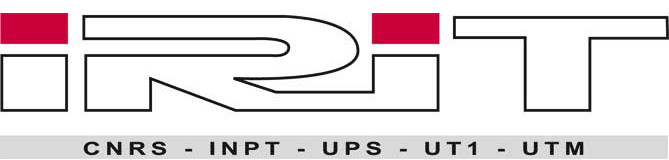
\includegraphics[width=0.28\textwidth]{logos/logo-irit.jpg}}
	\fancyhead[C]{} % On enlève les informations du header
	\fancyfoot[C]{} % On enlève les informations du footer
	\renewcommand{\headrulewidth}{0pt} % On enlève la ligne du header
} \Huge
\fancypagestyle{body}{%
	\restoregeometry 
	\pagestyle{fancy}
	\fancyhf{}
	\fancyhead[LO]{\ifthenelse{\equal{\value{chapter}}{0}}{}{\thesection. \rightmark}} %rightmark = section
	\fancyhead[RE]{\ifthenelse{\equal{\value{chapter}}{0}}
		{}
		{\textsc{Chapter} \thechapter.}
		\textsc{\leftmark}
	} %leftmark = chapter
	\fancyhead[RO]{\thepage} %
	\fancyhead[LE]{\thepage} %
	\renewcommand*{\chaptermark}[1]{\markboth{##1}{}}
	\renewcommand*{\sectionmark}[1]{\markright{##1}{}}
	\renewcommand\headrulewidth{.1pt}
	\setlength{\parskip}{0.2cm} % Espace entre paragraphes
%	\renewcommand{\arraystretch}{1.5} % Espace entre cases d'un tableau
}
\fancypagestyle{plain}{
	\pagestyle{body}
	\fancyhead[LO]{\rightmark}
}
\fancypagestyle{appendix}{%
	\restoregeometry
	% On nettoie les headers et footers existants de "fancy"
	\fancyhf{}
	% Pour le header
	\fancyhead[RE]{Appendix}
	\fancyhead[LO]{\thechapter. \leftmark} %leftmark = chapter
	\fancyhead[RO]{\thepage} %
	\fancyhead[LE]{\thepage} %
	\renewcommand*{\chaptermark}[1]{\markboth{##1}{}}
	\renewcommand\headrulewidth{.1pt}
	% Pour le footer
	%\fancyfoot[C]{\thepage}
	\renewcommand\footrulewidth{0pt}
} % <-- \pagestyle{body}
% MACROS

% Couleurs pour les corrections
\newcommand {\JY}[1] {\textcolor{red}{#1}}
\newcommand {\FR}[1] {\textcolor[rgb]{0.0,0.3,0.0}{#1}}
\newcommand {\OL}[1] {\textcolor{blue}{#1}}
\newcommand {\HW}[1] {\textcolor[rgb]{0.3,0.2,0.0}{#1}}
%\newcommand{\hilite}[1] {\emph{#1}}
\newcommand{\hilite}[1] {\Req{#1}}
\newcommand {\Req}[1] {\textcolor[rgb]{0.75,0.0,0.0}{#1}}
\newcommand {\Geq}[1] {\textcolor[rgb]{0.0,0.5,0.0}{#1}}
\newcommand {\Beq}[1] {\textcolor[rgb]{0.0,0.15,0.60}{#1}}
\newcommand {\black}[1] {\textcolor{black}{#1}}

% Espaces mathématiques
\newcommand {\DPUN} {{\mathcal D}}
\newcommand {\DTREE} {{\mathcal D}^e}
\newcommand {\CC} {\mathbb C}
\newcommand {\RR} {\mathbb R}
\newcommand {\RP} {\mathbb R^{\mathcal P}}
\newcommand {\RPE} {\mathbb R^{\mathcal P \times |\edges |}}
\newcommand {\codeset} {\mathbb R^{\mathcal P \times \leaves}}
\newcommand {\Dset} {\mathbb R^{\mathcal P \times (\mathcal P \#\leaves) }}
\newcommand {\ZZ} {\mathbb Z}
\newcommand {\NN} {\mathbb N}
\newcommand {\PP} {{\mathcal P}}
\newcommand {\HH} {{\mathbb H}}
\newcommand {\II} {{\mathbb I}}
\renewcommand {\SS} {{\mathcal S}} % applis supports
\newcommand {\SA} {{\mathbb S}} % support accessible

% Fonctions
\newcommand {\f}[1] { {\mathcal F}\left( #1 \right) }
\newcommand {\F}[1] { {\mathcal F^{-1}}\left( #1 \right) }
\newcommand {\norm}[2] {\left\| #1 \right\| _{#2}}
\newcommand {\defeq} {\triangleq}

% Opérateurs
\DeclareMathOperator {\sign} {sign}
\DeclareMathOperator {\prox} {prox}
\DeclareMathOperator {\argmin} {argmin}
\DeclareMathOperator {\supp} {supp}
\DeclareMathOperator {\rg} {rg}
\DeclareMathOperator {\diag} {diag}
\newcommand {\RG}[1] {\rg\left( #1 \right)}
\newcommand {\SUPP}[1] {\supp\left( #1 \right)}
\newcommand {\PS}[2] {\langle #1 , #2 \rangle}
\newcommand {\PROBA}[1] {\mathbb P \left( #1 \right)}
\newcommand {\one}[1] {\mathbbm{1}_{ #1 }}
%\newcommand {\one}[1] {\chi_{ #1 }} %{\mathbbm{1}_{ #1 }}
\newcommand {\oneinf}[1] {\chi_{ #1 }}
%\newcommand {\oneinf}[1] {{\mathcal I}_{ #1 }} 

% Acronymes
\newcommand {\PSNR} { \textrm{PSNR}^* } 
\newcommand {\NRE} { \textrm{NRE} }
\newcommand {\CPR} { \textrm{RER} }
\newcommand {\COST} { \textrm{G} } % ancien compression ratio

% Raccourcis
\newtheorem{prop}{Proposition}[section]

\newcommand {\nodes} {\mathcal N}
\newcommand {\edges} {\mathcal E}
\newcommand {\leaves} {\mathcal L}
\newcommand {\NL} {\#\leaves}
\newcommand {\hall} {h^e _{e \in \edges}}
%\newcommand {\multiconv}[1] { \bigstar_{\substack{#1}}\, }
\newcommand {\multiconv}[1] { \mathbf h^{#1}\, }
\newcommand {\tpath}[1] {\mathcal{C}(#1)}
\newcommand {\code} {\mathbf x}
\newcommand {\data} {\mathbf y}
\newcommand {\dataex} {\mathbf b}
\newcommand {\databis} {\mathbf y^e}
\newcommand {\D} {\mathbf D}
\newcommand {\Hs} {\mathbf A}
\newcommand {\Ha} {\mathbf H}
\newcommand {\Haf} {\hat{\mathbf H}}
\newcommand {\Hab} {\bar{\mathbf H}}
\newcommand {\res} {\mathbf r}

\newcommand {\tree}{\mathcal T}
\newcommand{\subtree}[1]{\tree^{#1}}

\newcommand {\stopalgo}{\epsilon}

% autres MACROS
\newcommand {\hkall} {(h^k)_{1 \leq k \leq K}}
\newcommand {\hkconv} {h^1 * \dots * h^K}
\newcommand {\hkconvnorm} {\frac{h^1}{\norm{h^1}{2}} * \dots * \frac{h^K}{\norm{h^K}{2}}}
\newcommand {\hkconvp} {g^{1} * \dots * g{K}}
\newcommand {\hkconvs} {f^{1} * \dots * f^{K}}
\newcommand {\fobj} {\| \code * h^1 * \dots * h^K - \data \|_2^2}
\newcommand {\fobjlambda} {\| \lambda \code * h^1 * \dots * h^K - \data \|_2^2}

% Macros added by Mael
\newcommand{\file}{\texttt}
\newcommand{\dispCode}{\texttt}
\newcommand{\dispCodeLong}[1]{
\begin{verbatim} #1 \end{verbatim}
}
\DeclareMathOperator*{\argmax}{\arg\!\max}% http://tex.stackexchange.com/q/83169/5764

\algnewcommand\algorithmicinput{\textbf{Input:}}
\algnewcommand\Input{\item[\algorithmicinput]}
\algnewcommand\algorithmicoutput{\textbf{Output:}}
\algnewcommand\Output{\item[\algorithmicoutput]}    % <-- \x, \y, \D...
% \newacronymwithdescr{Label}{Court}{Long}{Description}
\newcommand*{\newacronymwithdescr}[5][]{%
  \newglossaryentry{main-#2}{name={#3},%
  text={(\acs{#2}) #3\glsadd{#2}},%
  description={#5},%
  #1
  }%
  \newacronym{#2}{#3\glsadd{main-#2}}{#4}%
}

% Pas de point final pour les entrées glossaire ou acronymes
\setacronymstyle{sm-short-long}
%\newacronym{IMT}{IMT}{Institut de Mathématiques de Toulouse}
\newacronymwithdescr{IMT}{IMT}{Institut de Mathématiques de Toulouse}{is the main laboratory in mathematics in Toulouse}
\newglossaryentry{Blabla}{name=Blabla,description={is....}}

% To use the glossary entries:
% \acs{} (for short one)
% \ac{} (for long one - only on first appearence)

  % <-- acronyms (\ac{PALM}...)
\author{Maël Valais}
\date{Last revision on \gitAuthorDate{}}
\title{Optimization of Dictionaries Structured as Convolutional Trees for Sparse Image Representation - Master’s Thesis}
\begin{document}
\begin{titlepage}
\thispagestyle{pagedegarde}
\newgeometry{tmargin=2.2cm,bmargin=4cm,lmargin=2cm,rmargin=2cm}
\begin{center}
\topskip2.8cm
\textsc{Université Toulouse III — Paul Sabatier}\\
\vspace{0.5 cm}
\line(1,0){100}\\
\vspace{0.6 cm}
{{{Internship Report}}}\\
\vspace{0.3cm}
Defended on September 15\th, 2016\\ \vspace{0.3 cm} par\\ \vspace{0.3 cm} \textbf{Maël \textsc{Valais}}\\
\vfill
{\Huge \textbf{Optimization of dictionaries structured as convolutions trees for sparse image representation }}\\
\vfill

{{Internship at \acs{IMT}}}\\
{Université Paul Sabatier}\\
{118, route de Narbonne}\\
{31400 Toulouse}\\
\vspace{2 cm}

\par Supervised by \\ \textbf{François \textsc{Malgouyres}}\\
Institut de Mathématiques de Toulouse\\ 
%\vspace{1cm}
\par and \\Jean-Yves \textbf{ \textsc{Tourneret}}\\
ENSEIHHT, Toulouse
\end{center}
\end{titlepage}

% Préparation pour les pages de corps
\pagestyle{empty}
\restoregeometry
\cleardoublepage % Blanc jusqu'à prochaîne page paire

\tableofcontents
{\let\clearpage\relax\listoffigures}
{\let\clearpage\relax\listoftables}
{\let\clearpage\relax\listofalgorithms}

\pagestyle{corps} % Uncomment to show title page
\cleardoublepage % White until the next even page (if twoside)
\pagestyle{empty}
%{\let\clearpage\relax 
\begin{abstract}
This master’s thesis presents the algorithm OMP-PALMTREE for training fast dictionaries based on the convolutional tree model. Inspired by the construction of supports in OMP, this algorithm enhances PALMTREE by learning the supports (instead of fixing them). The  support adding step, as for OMP, is based on the maximum value of the gradient – which is shown to provide convincing indications on the best element that should be added. OMP-PALMTREE constitutes the “dictionary update” step in a standard dictionary learning algorithm, and must be associated with a “sparse coding” step (yet to be developed) for it to be used in applications like denoising or image recognition. Thanks to the convolutional tree model, dictionaries learned using OMP-PALMTREE are faster than dictionaries learned using a standard matrix-vector product (which yields quadratic computational cost), with a linear computational cost with respect to the size of the image.

\keywords{deep learning, dictionary learning, sparse image representation, non-convex optimization, machine learning, image processing}
\end{abstract}


\begin{foreword}[Foreword]
This master's thesis is the result of a six months internship  at the \ac{IMT} in the Mathematics for the Industry and Physics (MIP) team, in collaboration with the Signal and Communication (SC) team at IRIT\footnotemark[1]-ENSEEIHT\footnotemark[2]. This thesis is a requirement for the M2R Computer Science and Telecommunications, specialty “Operations Research” at the Paul Sabatier University (the courses are jointly taught at ENAC, INSA and ISAE-Supaéro).
\end{foreword}


\begin{foreword}[Acknowledgements]
First and foremost, I would like to extend my sincere gratitude to my research supervisors François Malgouyres, Jean-Yves Tourneret and Herwig Wendt for their enthusiastic encouragement and enlighten critiques. Thanks you,
\begin{enumerate}[label=--,noitemsep,nolistsep]
	\item François, for your kindness whatever the level of non-understanding I was going through;
	\item Jean-Yves, for your precious advice and your thorough corrections;
	\item Herwig, for being so demanding when commenting my manuscrits (I am good at writing vague sentences). I hope I am getting better!
\end{enumerate}

A big thanks to the mathematicians of the “Trainee Office” at IMT: Timothée Mathieu, Maylis Varvenne, Mickael Albertus and Laurence Denneulin. Special thanks to Timothée, who has excellent teaching skills and to whom I will be eternally grateful!

Finally, I wish to thank my fellows of the M2R “Operations research” (M2RIT\_RO15) 2015 promotion: Miezan Thomas, Luca Mossina, Benjamin Simon and Mustapha Ouaada. This was tough but so much worth it; I really enjoyed the many week-ends spent at ENAC\footnotemark[3] working together (and eating for cheap).

\begin{flushright}Maël Valais\end{flushright}

\footnotetext[1]{Institut de Recherche en Informatique de Toulouse}
\footnotetext[2]{École Nationale Supérieure d'Électrotechnique, d'Électronique, d'Informatique, d'Hydraulique et des Télécommunications}
\footnotetext[3]{École Nationale de l'Aviation Civile. This is the place where most of the M2RIT\_RO15 courses took place.}
\end{foreword}

% Document revision and last updated date
\begin{table}[hbt]\centering
  \begin{tabular}{>{\bf}rl}
   Document revision & \gitFirstTagDescribe{} \\
   Last updated on & \gitAuthorDate{} \\
   Author & \gitAuthorName{} (\gitAuthorEmail{})
  \end{tabular}
\end{table}
\vskip 2cm


\tableofcontents
%{\let\clearpage\relax\listoffigures}
%{\let\clearpage\relax\listoftables}
%{\let\clearpage\relax\listofalgorithms}

\restoregeometry
\pagestyle{fancy}
\pagestyle{body}
\chapter{Introduction}

A sparse signal over some representation means that it can be expressed using only a few elements of the representation – in other words, sparse means with many zero coefficients. Many applications ranging from machine learning to image denoising and image recognition heavily rely on the property that we can summarize (or more exactly approximate) any signal using a proper sparse representation. The job of obtaining the original signal from its sparse counterpart can be written in terms of an operator, often called \emph{dictionary} or \emph{transform}. 

\noindent
In this introductory chapter, we introduce and review the main existing dictionaries that have been used for sparse representations, from non-adaptive transforms to learned dictionaries via the intermediate over-complete dictionaries. The second part of this chapter provides the motivations and general objectives of this work as well as the related works.

\section{Basis and redundant dictionaries}

The \ac{DFT} is a classical example of an operator used for sparsity. The \ac{DFT} can be written as a matrix $\D$, where $\D$ denotes the dictionary. Finding the Fourier representation – which we will refer to as the \emph{code} $\x$ – of an image $\y$ amounts to compute 
\begin{equation}\x = \D^T\y.\label{eq_matrixvector}\end{equation}

\begin{figure}[!ht]
\subcaptionbox{Picture $\y$ with many discontinuities.}%
  [.49\linewidth]{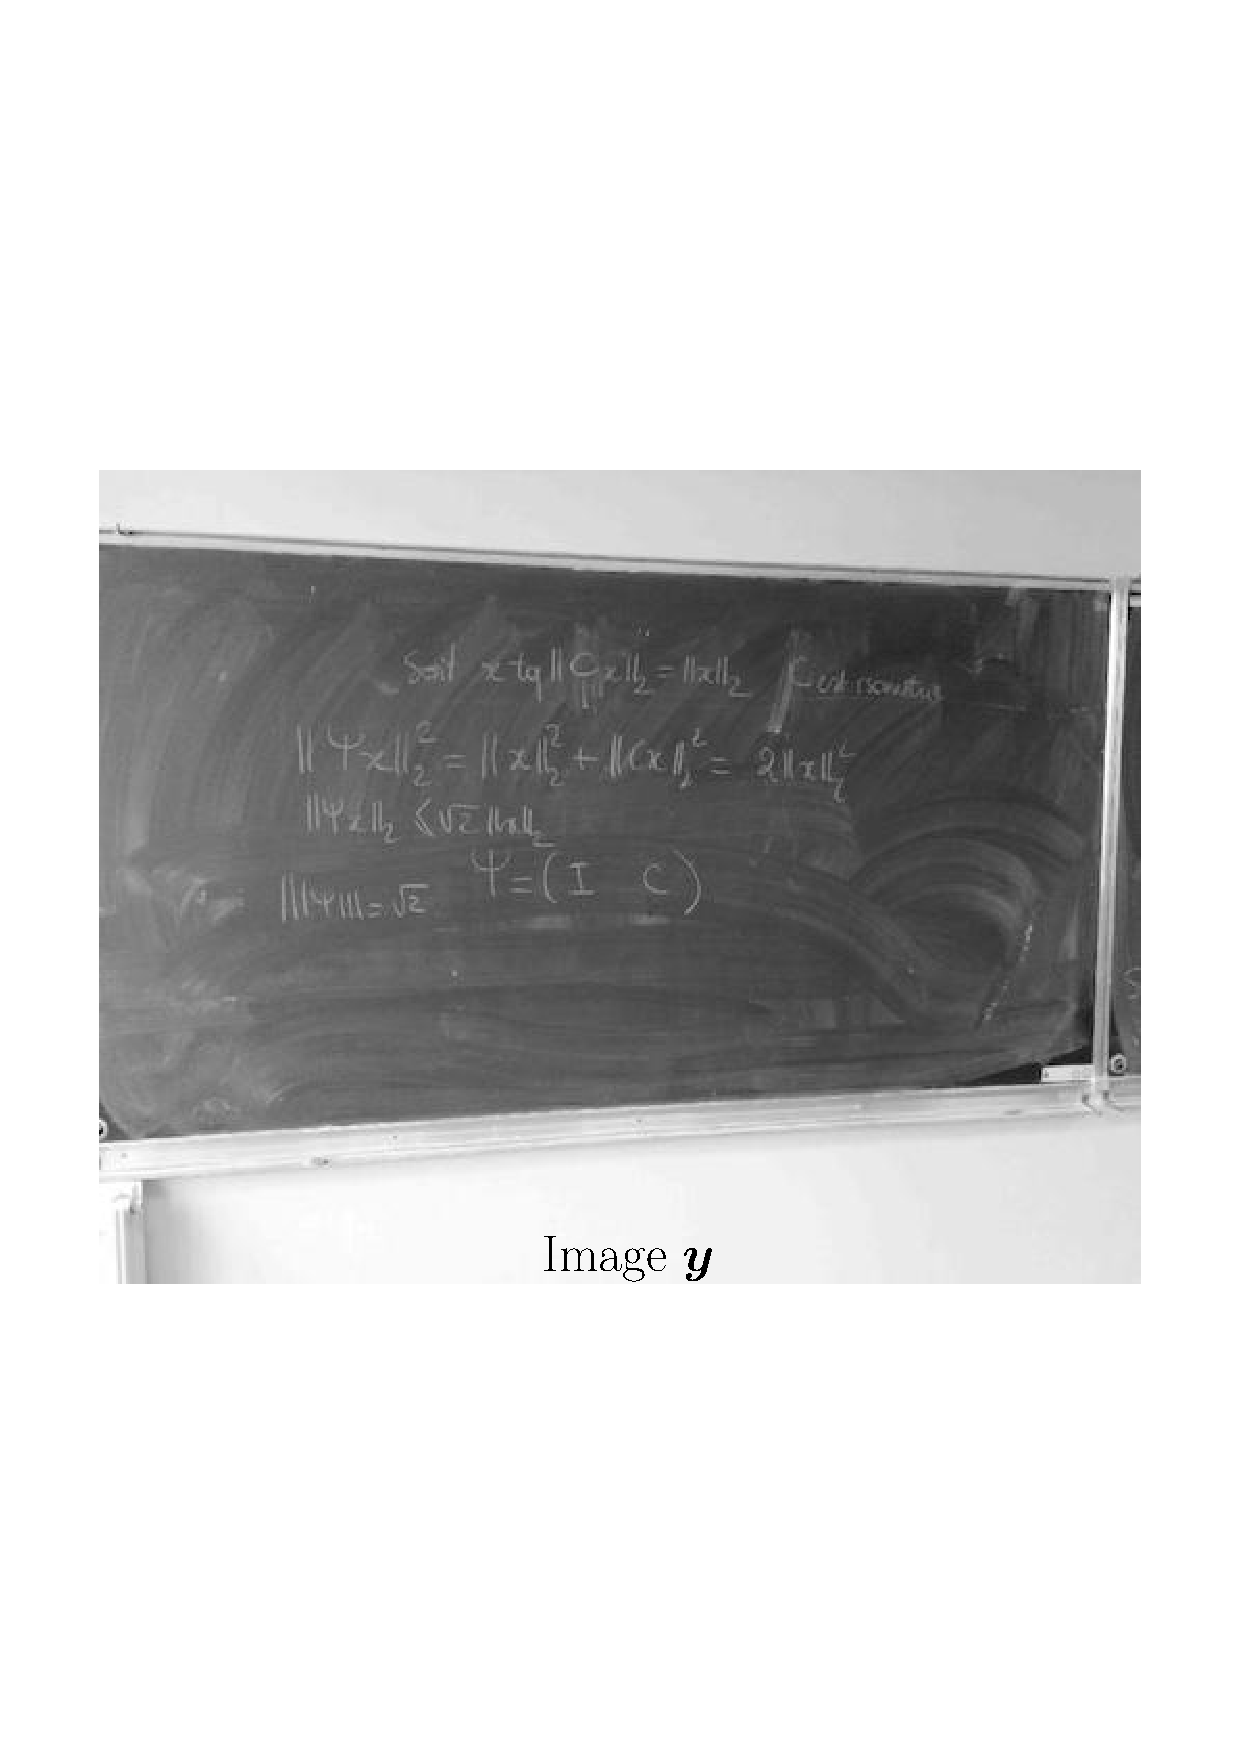
\includegraphics[width=0.49\textwidth]{figures/fourier/image.pdf}}
 \subcaptionbox{Result of applying the Fourier transform to $\y$}%
  [.49\linewidth]{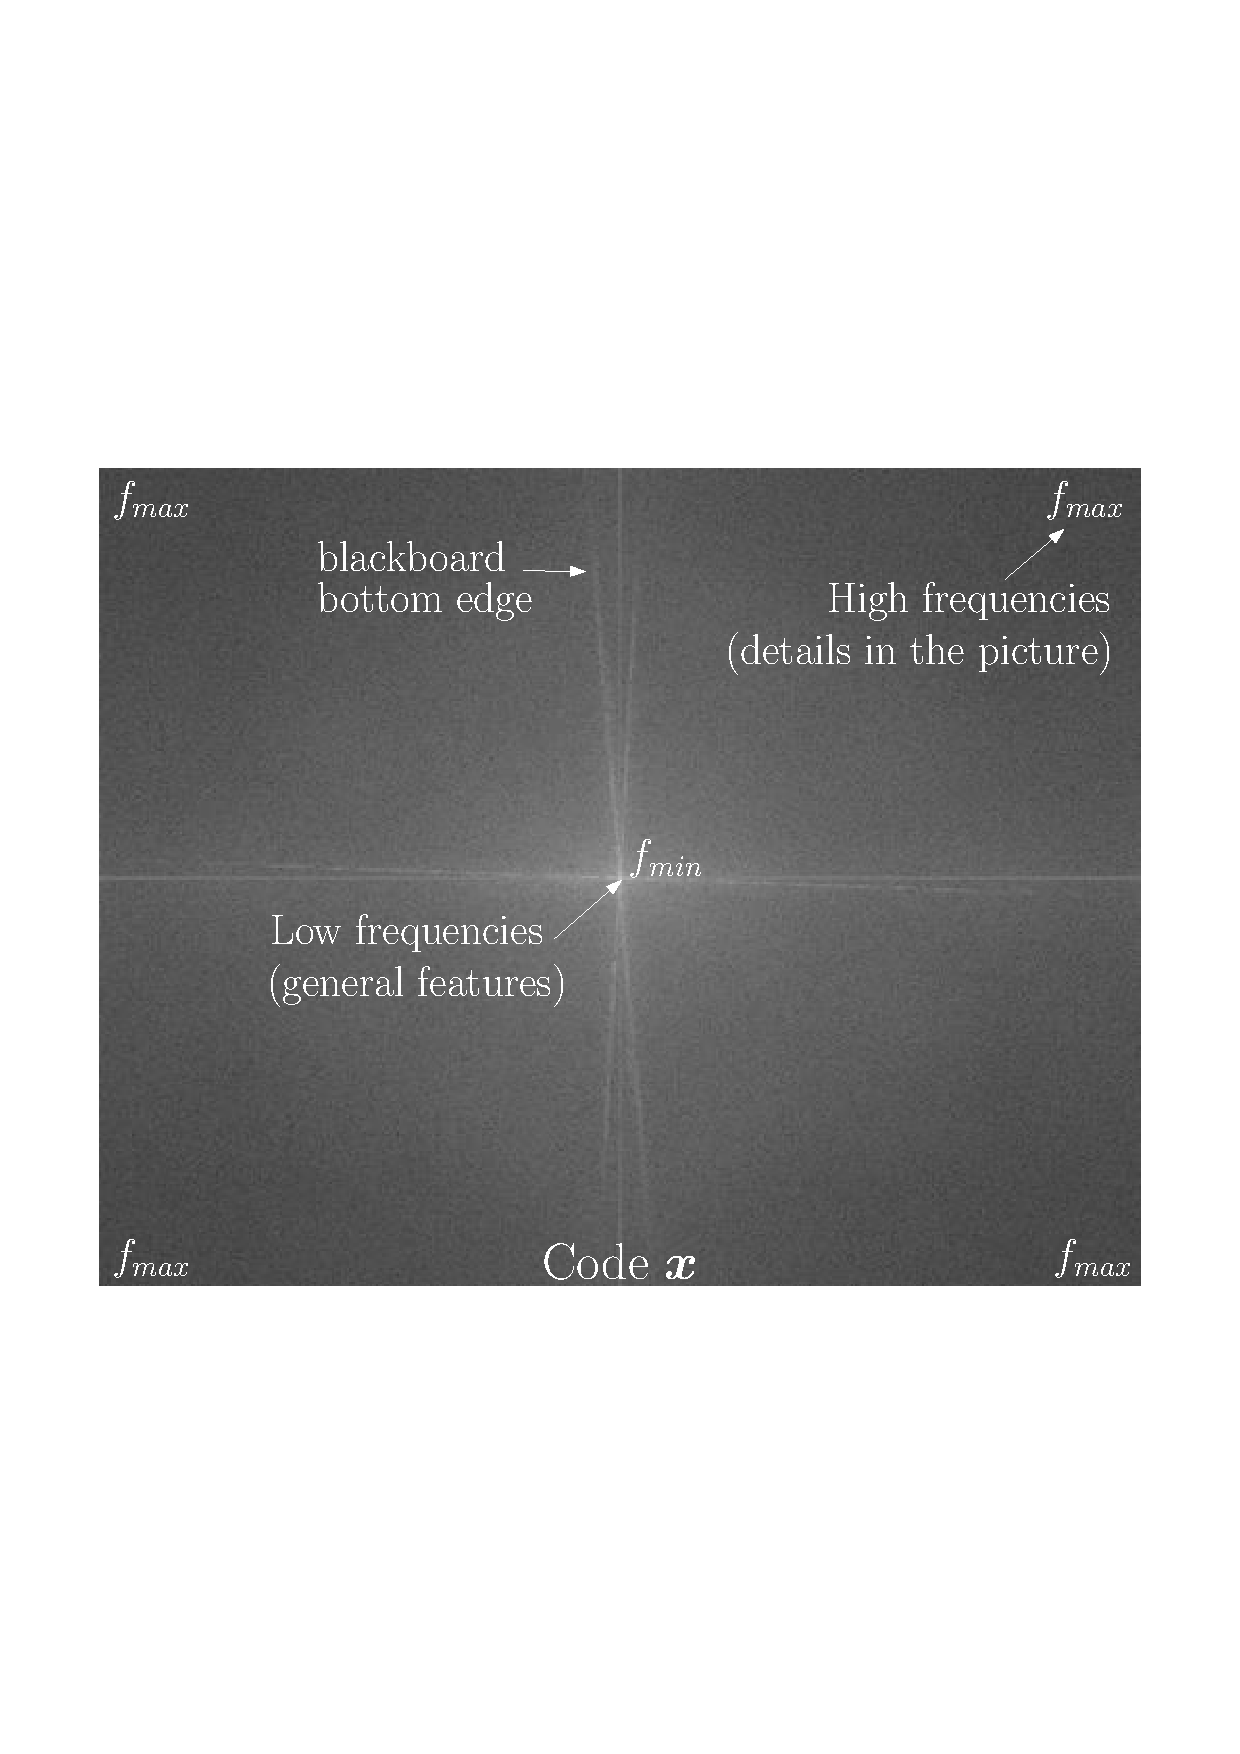
\includegraphics[width=0.49\textwidth]{figures/fourier/fourier.pdf}}
  \caption{Decomposition $\D^T\y=\x$ of a signal $\y$ using the dictionary $\D$ made of Fourier series. In $\x$, the middle coefficients are coding “large” features while the corner values are coding the details. The multiple white lines, ranging from the middle to the borders, outline the discontinuities caused by the blackboard edges; these coefficients are scattered (hence not sparse), which shows that the Fourier basis has representation problems in presence of discontinuities.}\label{fig_fourier}
\end{figure}

\noindent
However, the Fourier transform is quite different from the representations we have in mind, namely the convolutional tree structures. First, Fourier coefficients form a basis, implying that it is a one-to-one representation in the sense that every code $\x$ is associated with a unique image $\y$ and vice versa. This basis is also orthonormal, implying that the operator is stable (it does not amplify errors), as well as normalized (each element has a norm equal to 1).

\noindent
More importantly, the \ac{DFT} has interesting properties that allow fast implementations. For example, applying the Matlab function \texttt{fft2} to the \cref{fig_fourier} takes less than a millisecond. If we assume $N$ to be the dimension of the concatenated\footnotemark[2] (also referred as “vectorized”) image, instead of computing a time-expensive $\O(N^2)$ matrix-vector product as in \eqref{eq_matrixvector}, the fast Fourier transform only requires a computational cost of the order $\O(N \log N)$.

\footnotetext[2]{We consider 2-D images as one-dimensional vectors: an image of size $16 \times 16$ would give a \emph{concatenated} (or \emph{vectorized}) vector of length 256.}

\noindent
The Fourier transform is widely used as an operator for sparse representations, mainly when dealing with smooth signals that can be approximated by a sum of sinusoids. However, this operator does not generally perform well on images since they contain many discontinuities that are far from being sparsely representable using sinusoids.

\noindent
The problem with discontinuities is illustrated in \cref{fig_fourier}. As an example, the bottom edge of the blackboard (which is a strong discontinuity) induces a long vertical trail of large coefficients in $\x$. Because of discontinuities, $\x$ is forced to have many non-zero coefficients. 

\noindent
Along with Fourier, many other basis dictionaries exist; we can mention the cosine transform which is at the core of JPEG compression. We can also cite the wavelet transform, used in JPEG2000 compression. Note that both wavelets and cosine have fast implementations.

\section{Redundant dictionaries}

Basis dictionaries were generalized by using multiple bases to form a stable and redundant (also called over-complete) dictionary in \cite{shaobing_chen_atomic_2001}. For example, combining a canonical basis with a cosine basis allows both peaks and sinusoids to be represented.

\noindent
Other redundant dictionaries, like the curvelet transform, do not have the useful properties of bases, yet are stable and have fast implementations. It is interesting to note that contrary to Fourier or cosine transforms, the curvelets can code (to an extent) non-smooth signals.

% Notes for myself
% 1. tight frame = preserves the norm
% 2. orthogonality preserves the norm (norm doesn’t make the errors explode)
% 3. orthogonal means that it is stable

\noindent
Although offering excellent performances for sparse representations thanks to their fast implementations, redundant dictionaries have the drawback to lack adaptivity.


\section{Learned dictionaries}
Previously mentioned dictionaries are said to be “non-adaptive,” meaning that they are not specific to any data and can lead to a non-optimal code sparsity (as explained above in \cref{fig_fourier}). Dictionary learning allows us to create “adaptive” dictionaries, i.e., data-driven dictionaries. Instead of being fixed, the atoms of an “adaptive” dictionary are based on a learning set of example images, denoted by
\begin{equation*}\Y = \begin{bmatrix} \y_1 & \dots & \y_S \end{bmatrix}\end{equation*}
where the columns of $\Y$ are the vectorized images $\y_i \in \R^N$, and $S$ the number of sample images. The dictionary $\D$ is made of $K$ columns $\d_i$ (the atoms) such that the number of atoms is much larger than the dimension of a single image $\y_i$ ($K \gg N$):
\begin{equation*}\D = \begin{bmatrix} \d_1 & \dots & \d_K \end{bmatrix}.\end{equation*}
The codes $\X$ are defined by
\begin{equation*}\X = \begin{bmatrix} \x_1 & \dots & \x_{S} \end{bmatrix}\end{equation*}
where $\X$ is the concatenation of $S$ column vectors $\x_i$ (the codes for each image in $\Y$) of length $K$. The dictionary learning problem is defined as
\begin{align}
\underset{\D,\X}{\min}~ & \lVert \X \rVert_1 + \lambda\lVert \D\X-\Y \rVert^2_F \tag{$DL$}\label{eq_dl} \\
\text{s.t.}~ & \lVert \d_k \rVert \le \gamma & \forall k = 1,\dots,K\label{eq_dl_finite_norm}
\end{align}
where $\lVert . \rVert_F$ denotes the Frobenius norm and $\lVert . \rVert_1$ is the $l_1$ norm defined by $\|\X\|_1  = \sum_{i=1}^S \sum_{j=1}^K |x_i^j|$.
Note that the constraint \ref{eq_dl_finite_norm} prevents the atoms from having an arbitrarily large norm.

\noindent
The problem \eqref{eq_dl} can be understood as finding the atoms of $\D$ that give a sparse representation $\x_i$ approximating $\y_i$ for all $i = 1,\dots,S$. This approximation is denoted as
\begin{equation*}\D\X \approx \Y.\end{equation*}

\noindent
\Cref{fig_overcomplete_matrix} gives an idea of what we mean by approximating an image $\y$ using the matrix-vector product of a sparse code $\x$ and a learned dictionary $\D$. For this example, $\y$ is represented by a linear combination of three atoms of $\D$: $\x$ is 3-sparse.

\begin{figure}[!ht] \centering
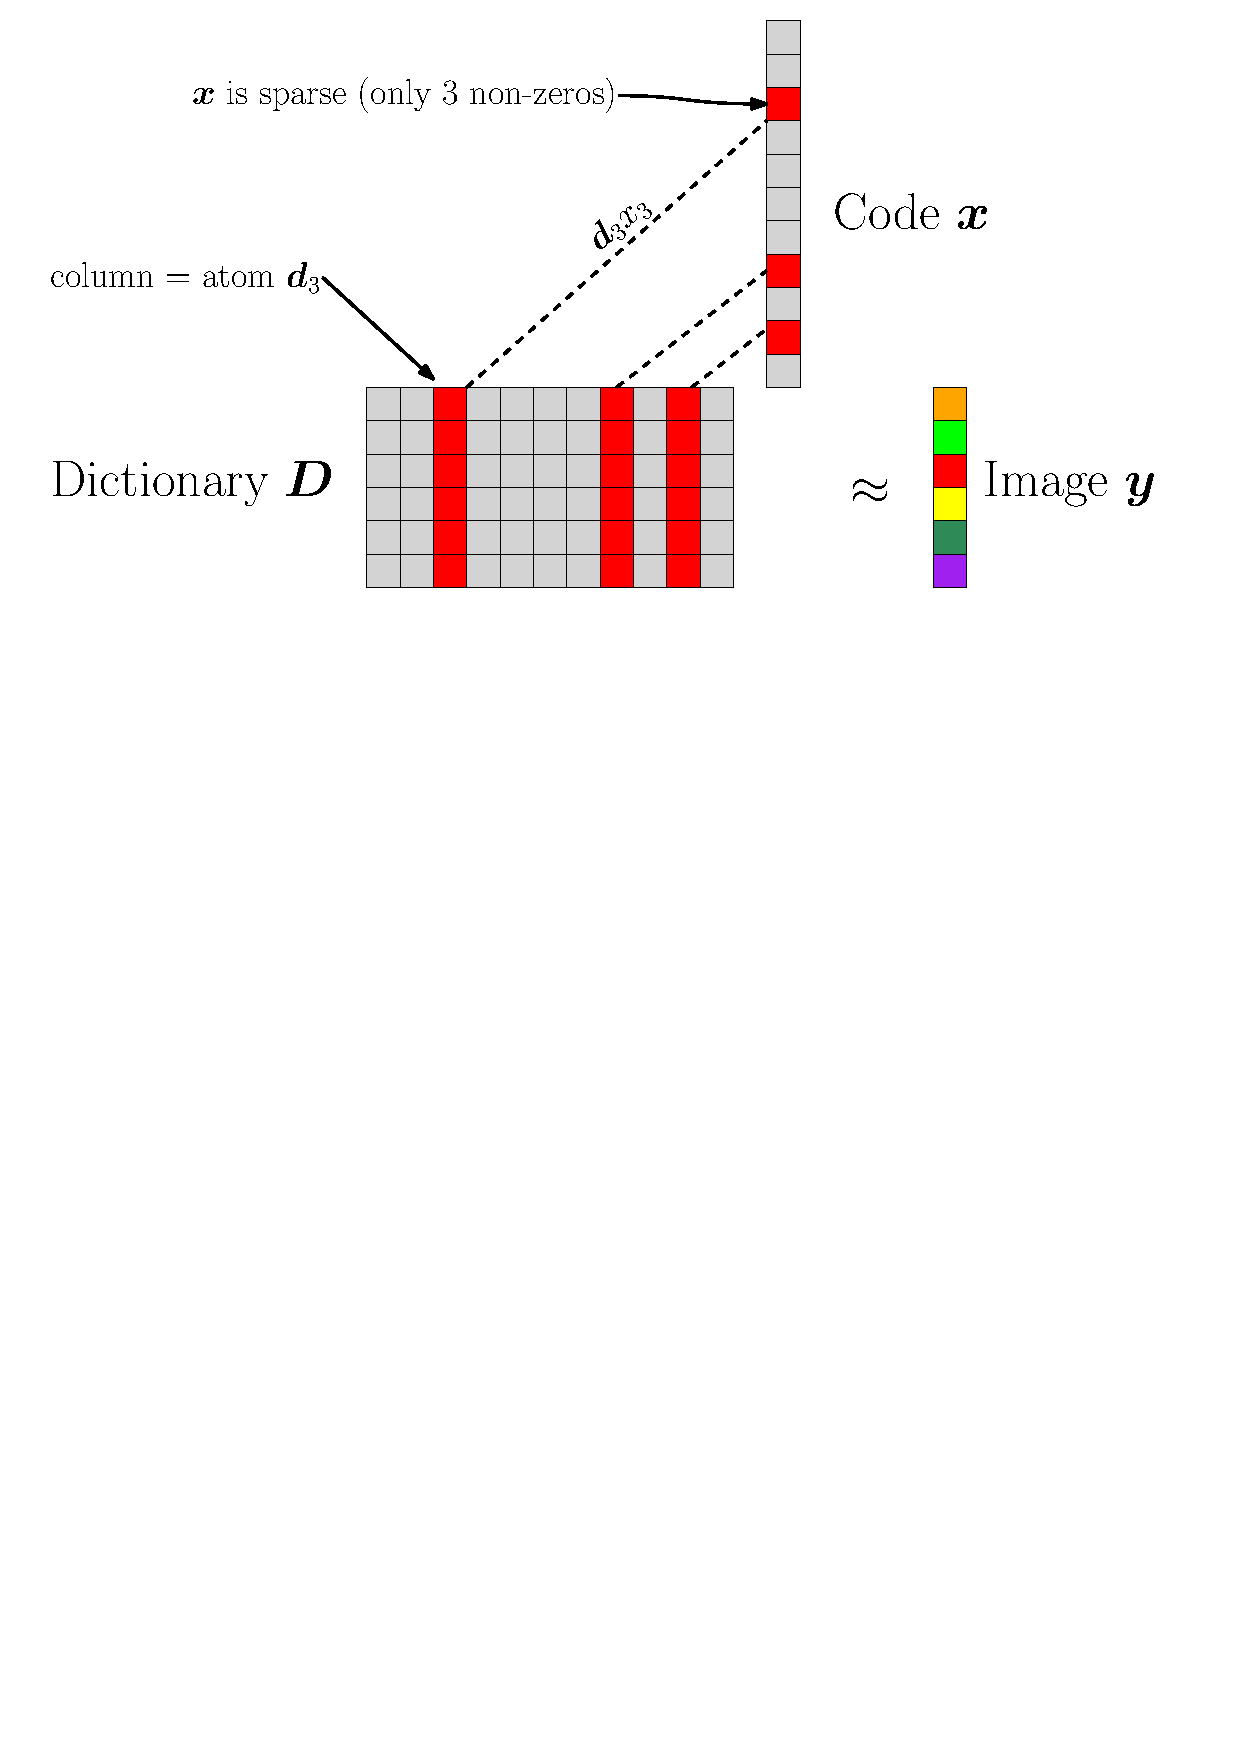
\includegraphics[width=0.90\textwidth]{figures/sparsity-matrix.pdf}
\caption{Matrix view of $\D\x$ when $\D$ is over-complete (much more columns than lines) and $\x$ is sparse.}\label{fig_overcomplete_matrix}
\end{figure}


Note that the non-linearity caused by the product $\D\X$ induces a non-convex objective function for the unknowns $\D$ and $\X$, making it difficult to optimize simultaneously with respect to $\D$ and $\X$. To work around this problem, many algorithms solve \eqref{eq_dl} by optimizing alternatively with respect to the dictionary $\D$ and the codes $\X$ (referred to as the dictionary update and sparse coding step, respectively).

\subsection{Existing dictionary learning algorithms}
Among the many available algorithms (and their multiple versions) for dictionary learning, the \ac{KSVD} algorithm is a typical example. Introduced in \cite{aharon_k-svd:_2006} and inspired by the widely known \gls{KMeans} algorithm, it is used in many image processing applications. This algorithm is detailed in the next section.

\noindent
More scalable algorithms are given by the class of “online” dictionary algorithms. An online dictionary learning algorithm, such as the one proposed in \cite{mairal_online_2010}, learns one image after the other instead of learning the whole set of images simultaneously. Thus, it is very suitable for huge sets of learning images.

\noindent
For a thorough review of every transform available (developed before 2010), the reader is invited to take a look at  \cite{rubinstein_dictionaries_2010}.


\subsection{Example with the \acs{KSVD} algorithm}

Among the many existing alternating algorithms for dictionary learning, the \ac{KSVD} algorithm is well known for its state-of-the-art performance in image denoising. \ac{KSVD} is responsible of many concepts behind the \acs{PALMTREE} algorithm (the algorithm developed in \cite{chabiron_optimization_2016} and that we are trying to improve). This section summarizes the key elements of the \ac{KSVD} algorithm.

\ac{KSVD} does not actually solve \eqref{eq_dl}; instead, it seeks a solution for a “stronger” problem in the sense that the level of sparsity in \ac{KSVD} is enforced by $\gamma$, leading to the following problem
\begin{align*}
\underset{\D,\X}{\min}~ & \lVert \D\X-\Y \rVert^2_F \tag{$DL_2$}\label{eq_dl_ksvd} \\
s.t.~& \lVert \x_i \rVert_0 \le \gamma & \forall i \in 1,\dots,S
\end{align*}
where $\lVert . \rVert_F$ denotes the Frobenius norm and $\lVert . \rVert_0$ is the pseudo-norm $l_0$ (also known as “counting function”).

\noindent
The \emph{Sparse Coding step} optimizes the cost function with respect to $\x$; this step basically uses \ac{OMP} (detailed in \cref{alg_omp}) or any other pursuit algorithm. The \emph{Dictionary Update step} optimizes the cost function w.r.t.\@ $\D$. This is the step that was studied in \cite{chabiron_optimization_2016}. Note that the full \ac{KSVD} algorithm is presented in \cref{sec_ksvd_detail}, \cpageref{sec_ksvd_detail}.

\noindent
\Cref{fig_ksvd} gives an example of what “learning $\D$” with the \ac{KSVD} algorithm means. As the image (a) is too big ($512 \times 512$) to be learned directly, we must chop it into many small patches, e.g., of size $16 \times 16$. \Cref{fig_ksvd_patches} shows some of these patches contained in $\Y$, which actually holds 10240 patches ($\Y$ has dimension $128 \times 10240$). The dictionary $\D$ of size $128 \times 128$ (it has 128 atoms) is shown in (c). Note that $\D$ has been learned with a sparsity of 10 and that the process took about five minutes (stopped after 20 iterations).

\noindent
The dictionary in \cref{fig_ksvd_dict} can now be used for denoising the noisy image of \cref{fig_ksvd_image}. If we would like a dictionary for image recognition or compression, we would probably need many additional images in order to obtain a good classification or compression performance.

\begin{figure}[!ht]\centering
\begin{subfigure}[b]{0.40\textwidth}\centering
	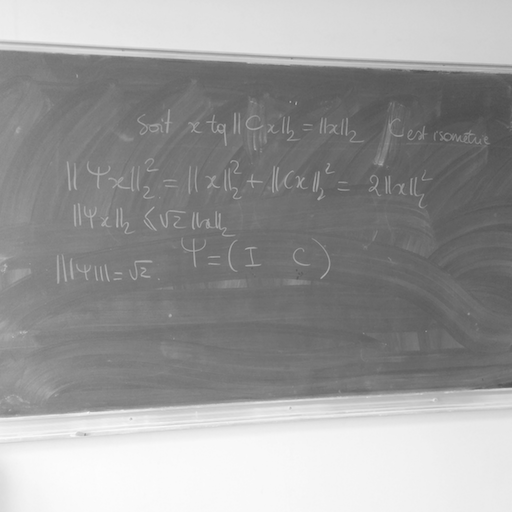
\includegraphics[width=\textwidth]{figures/ksvd/tableau_512x512.png}
	\caption{Image used for learning}\label{fig_ksvd_image}
\end{subfigure}
\begin{subfigure}[b]{0.29\textwidth}\centering
	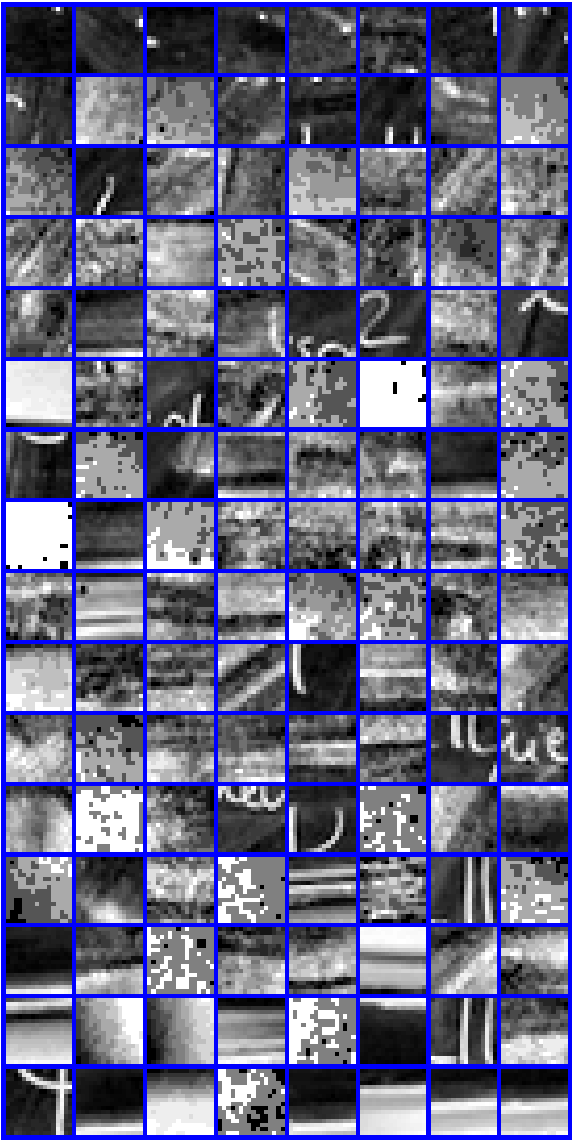
\includegraphics[width=0.7\textwidth]{figures/ksvd/patches.pdf}
	\caption{Image patches $\Y$}\label{fig_ksvd_patches}
\end{subfigure}
\begin{subfigure}[b]{0.29\textwidth}\centering
	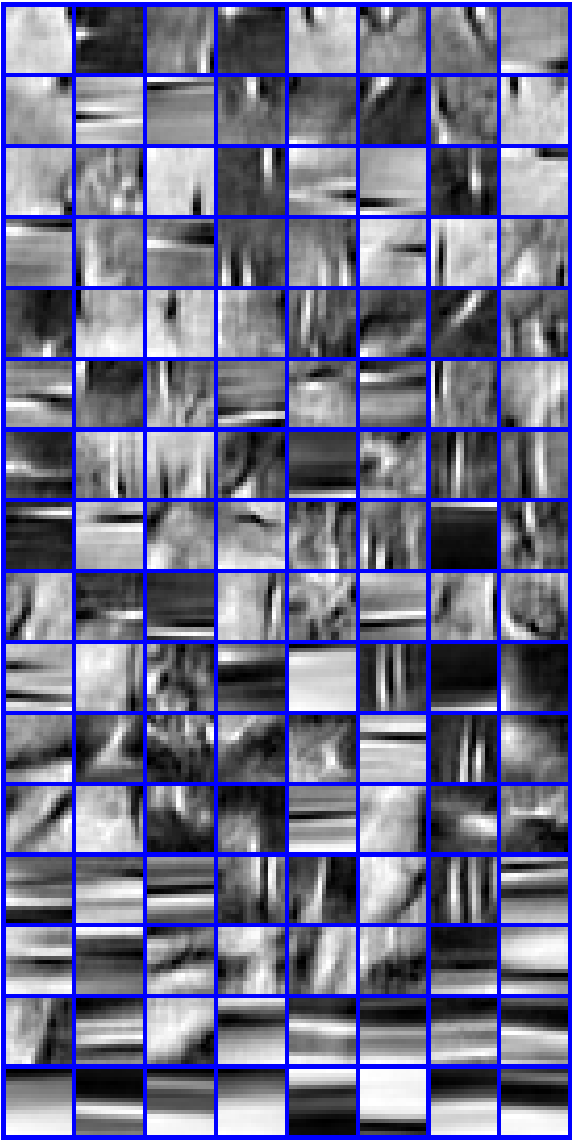
\includegraphics[width=0.7\textwidth]{figures/ksvd/dictionary.pdf}
	\caption{Learned $\D$}\label{fig_ksvd_dict}
\end{subfigure}
\caption{Learning $\D$ on image patches using \ac{KSVD}.}\label{fig_ksvd}
\end{figure}


\subsection{Problem of atom scalability: multi-scale dictionaries}
As the learned \ac{KSVD} dictionary relies on the $\O(N \cdot K)$ matrix-vector product and has to be over-complete ($K \gg N$) in order to achieve sparsity, we easily understand that $N$ cannot take an arbitrarily large value. In practice, the example images (the patches) and atoms of the dictionary are generally of size at most $16 \times 16$.

\noindent
Dictionaries with bigger atoms are known as multi-resolution (also called multi-scale), meaning that the atoms can contain either details or large features computed from the images.


\subsection{Problem of atom redundancy: convolutional dictionaries}\label{sec_atoms_redund}
The \ac{KSVD} algorithm is not translation-invariant in the sense that multiple atoms of the dictionary can have the same detail but slightly translated. The authors of \cite{mailhe_shift-invariant_2008} worked on making the update step invariant by translation, but it still needs a lot of tuning and finding the right parameters.

\noindent
Translation-invariant transforms are known as convolutional dictionaries. Instead of having (possibly) multiple atoms that contain the same feature at different places, convolutional dictionaries contain all possible translations for every atom; contrary to traditional learned dictionaries, it is unlikely to find two atoms containing the same detail with different locations.

\noindent
Many state-of-the-art machine learning techniques are based on trees of convolutions, such as the Convolutional Neural Networks used in Deep learning \cite{lecun_deep_2015}.

\section{Research motivations and general objectives}
Sparse representations have been used successfully in many applications. The use of these representations is only limited by the performance of their transforms. By performance, we mean that the transform must be
\begin{enumerate}[label=--,noitemsep,nolistsep]
\item fast (fast computation of $\D\x$),
\item adaptive (must be learned on a set of images)
\item and stable (does not amplify errors).
\end{enumerate}

\noindent
As mentioned, many algorithms are available in the literature. However, they are often fast but not adaptive (such as the Fourier transform) or adaptive and not fast (such as \ac{KSVD}).

\noindent
The main general objective of this work is to develop a multi-resolution dictionary model (allowing large atoms to be considered) that is fast and adaptive, based on the principle of convolutional trees. During his PhD thesis, Olivier Chabiron has been working on a \gls{treemodel}, presented in the paper \citetitle{chabiron_optimization_2016} (\cite{chabiron_optimization_2016}). Our work focuses on improving this model in order to (eventually) solve the \eqref{eq_dl} problem.


\section{Related work}
Among others, we mention two teams that are currently actively working on multi-resolution transforms:
\begin{itemize}
	\item[--] the team lead by Mickeal Elad proposed a dictionary model based on wavelets in \cite{sulam_trainlets:_2016};
	\item[--] Rémi Gribonval’s team has proposed a factorization-based dictionary model in  \cite{le_magoarou_flexible_2016}.
\end{itemize}
Their work have been published very recently (in early 2016); this master's thesis does not consider the approaches investigated in these papers. However, studying these advances will be conducted just after the end of this internship during a PhD thesis.





\chapter{State of the art}

In the previous chapter, we reviewed the various available dictionaries along with their strengths and weaknesses. More specifically, we studied an algorithm, \ac{KSVD}, that yields state-of-the-art dictionaries in term of adaptiveness, although being notably slow because of its unstructured matrix.

\noindent
This chapter introduces a different dictionary model, namely the \gls{treemodel}, that is intended to produce adaptive as well as fast dictionaries thanks to a tree structure. Along with this model, we present the associated dictionary learning problem, \acs{FTL}, and the algorithm \ac{PALMTREE} that solves this problem. The end of this chapter is dedicated to detailing the specific objectives of this internship.

\section{Dictionary structured by the \gls{treemodel}}\label{sec_tree_model}
The work studied in \cite{chabiron_toward_2015} and \cite{chabiron_optimization_2016} offers a different way of structuring the matrix $\D$, namely the \emph{\gls{treemodel}}. Instead of using “plain” atoms as columns and dealing with the matrix-vector product with complexity $\O(N \cdot K)$, $\D$ is defined by a convolutional tree structure \begin{equation*}\T(\V,\E).\end{equation*} 
To each edge $e$ of $\E$ is associated a kernel $\h^e$ and a support $\s^e$. The leaves $l \in \L \subset \V$ associated with the root $r \in \V$ allow us to define a branch as the successive edges growing from the root (top) to one of the leaves (bottom).

\begin{figure}[!ht]\centering
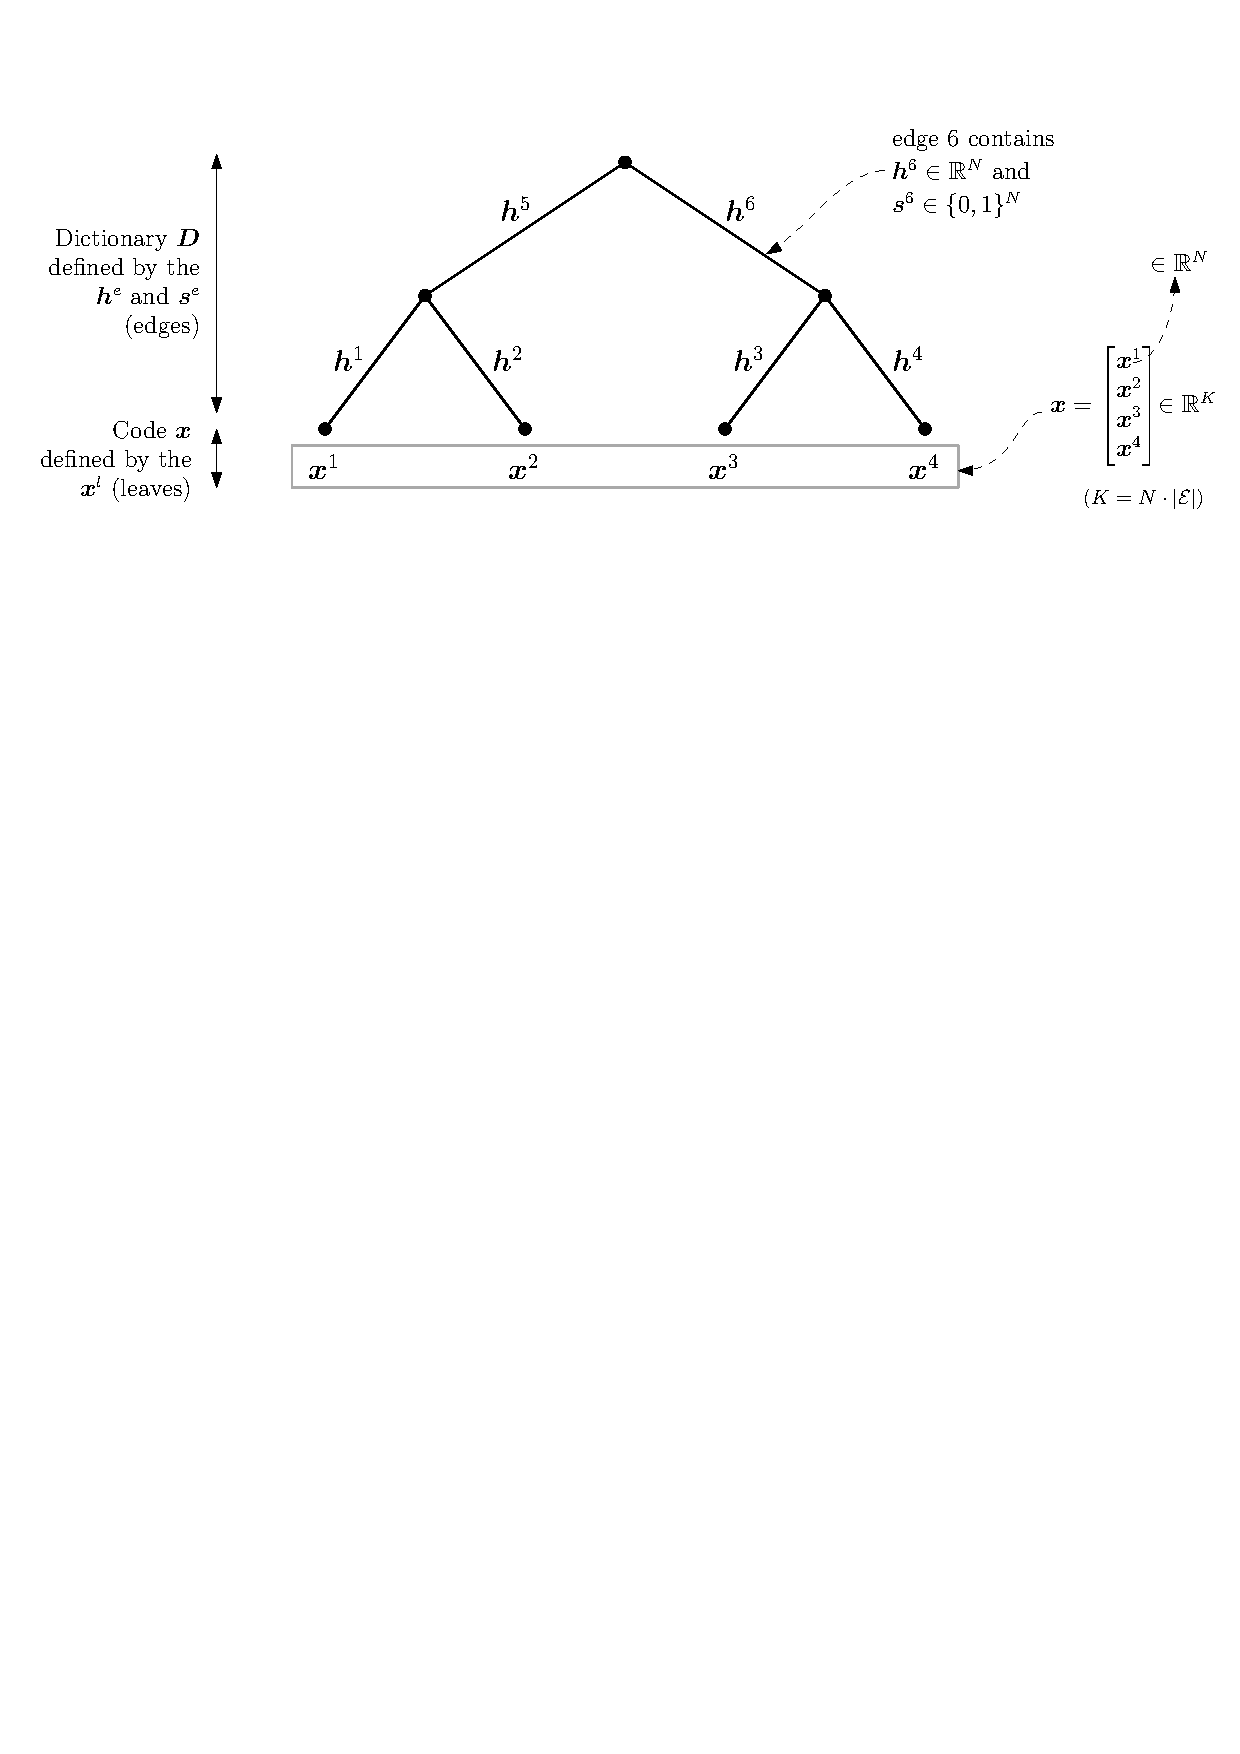
\includegraphics[width=\textwidth]{figures/tree.pdf}
\caption{View of a convolutional tree; the $\h^e$ and $\s^e$ are what define $\D$. $|\L|$ denotes the cardinal of set $\L$.}\label{fig_tree}
\end{figure}

\noindent
The target image $\y$ as well as the kernels $\h^e$ and supports $\s^e$ are vectors of dimension $N$. The supports $\s^e$ only take the values 0 (corresponding value in $\h^e$ must be 0) or 1 (corresponding value in $\h^e$ can be non-zero). For easier reading, we will denote the families $(\h^e)_{e \in \E}$ and $(\s^e)_{e \in \E}$ by \begin{equation*}\h = (\h^e)_{e \in \E}\end{equation*} and \begin{equation*}\s = (\s^e)_{e \in \E}.\end{equation*}

The code $\x$ is a “big” vector of length $K$ with $K = N \cdot |\L|$ such that \begin{equation*}\x = \begin{bmatrix}x_{11} \\ \vdots \\ x_{|\L|N}\end{bmatrix} \quad \text{with $x_{lp}$ the coefficient of $\x$ at leaf $l$, point $p$.}\end{equation*} 
Finally, the dictionary matrix associated\footnote{The convolutional tree dictionary can be rewritten into a matrix; see \cref{sec_matrix_vs_tree}} with the \gls{treemodel} is denoted $\D$ and is of dimension $N \times K$, and the image $\y$ is a vector of length $N$.

\noindent
In the following, we will denote the image space using the notation
\begin{equation*}\P = \{p ~|~ p=1,\dots,N\}\end{equation*}
and the image $\y$ will be defined as
\begin{equation*}\y = \begin{bmatrix}y_1 \\ \vdots \\ y_N\end{bmatrix} \quad \text{with $y_p$ the $p$-th coefficient of $\y$.}
\end{equation*}

\noindent
For convenience, the images $\h^e$, $\x^l$ and $\y$ are defined as “circular” or “periodic” signals, meaning that they are defined for every $p \in \mathcal{Z}$. With that in mind, we can define the circular convolution for two circular signals $\h$ and $\h’$ of $\R^N$ as
\begin{equation*}(\h * \h’)_p = \sum_{p’ \in \P} \h_{p-p’} \h’_{p’}\end{equation*}

\begin{figure}[!ht]\centering
\begin{subfigure}[b]{0.20\textwidth}\centering
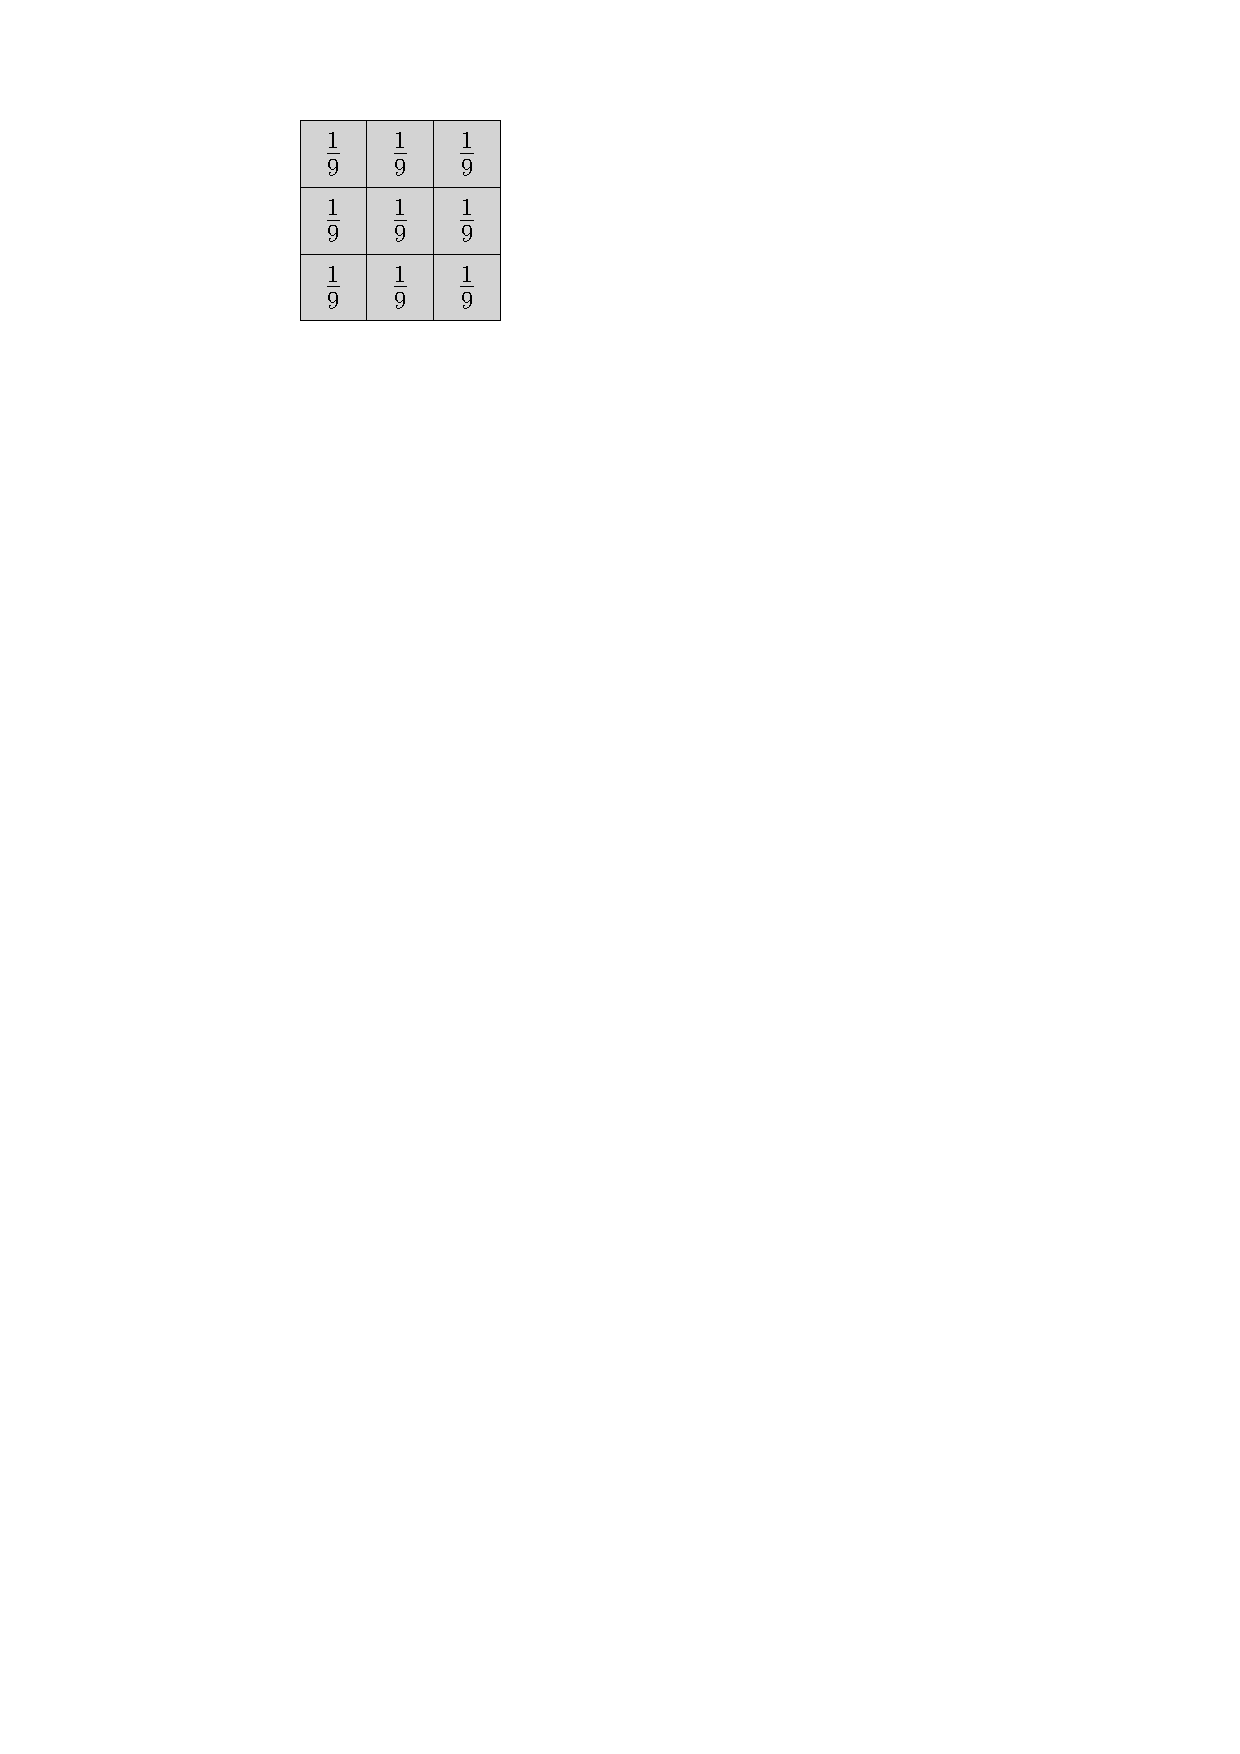
\includegraphics[width=0.90\textwidth]{figures/kernel-exple.pdf}
\caption{Averaging kernel: fixed support and values}
\end{subfigure}
\begin{subfigure}[b]{0.79\textwidth}\centering
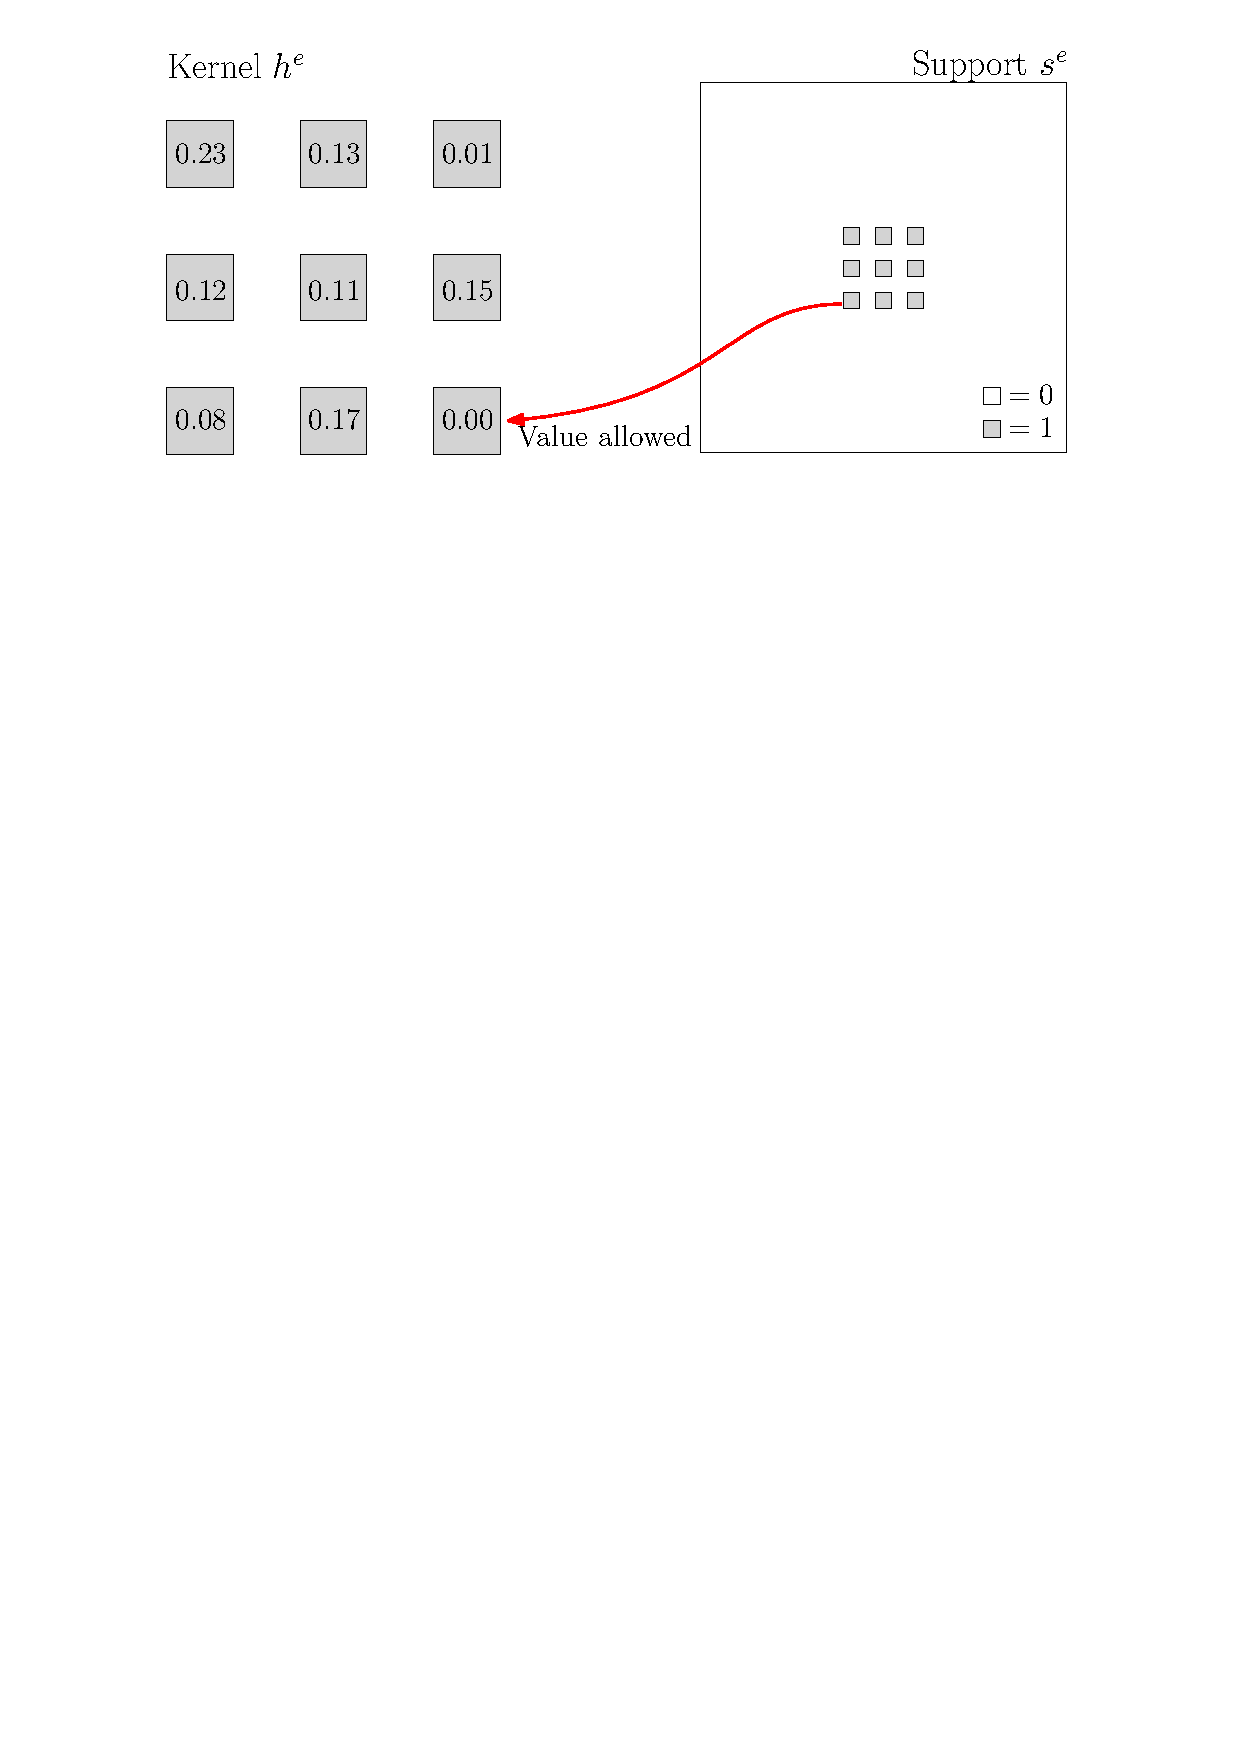
\includegraphics[width=0.90\textwidth]{figures/kernel-h_e.pdf}
\caption{Kernel $\h^e$ (left) and its associated support $\s^e$ (right).}\label{fig_example_kernel-h_e}
\end{subfigure}
\caption{Two examples of convolutional kernels.}\label{fig_example_kernel}
\end{figure}

\noindent
\Cref{fig_example_kernel-h_e} displays examples of a standard kernel (left) and a kernel $\h^e$ (middle) associated with its support $\s^e$ (right). The gray squares represent the “ones” of the support while the kernel is represented by values inside the squares.

\noindent
We denote the convolution of successive kernels on a given branch identified by the leaf $l$ by
\begin{equation*}\h^{*l} = \h^r * \dots * \h^l.\end{equation*}

\noindent
Instead of using the standard matrix-vector product, the convolutional tree dictionary computes $\D\x$ as follows
\begin{align}
	\D\x = \sum_{l \in \L} \x^l * \h^{*l}.\label{eq_Dx_as_conv}
\end{align}

\section{The \acs{FTL} problem}

The dictionary update step associated with the \gls{treemodel} is defined as
\begin{align}
\underset{\substack{(\h^e)_{e}}}\min ~ & \lVert \D\x - \y \rVert_2^2 \tag{$FTL$}\label{eq_ftl}\\
\text{s.t.~} & \s^e_p=0 \Rightarrow \h^e_p = 0 \quad & \forall p=1,\dots,N ,~\forall e \in \E\label{eq_ftl_in_support} \\
 & \lVert \h^e \rVert \le \gamma & \forall e \in \E.\label{eq_ftl_kernel_finite_nrj}
\end{align} 
Note that the \glsdisp{FTL}{Fast Transform Learning (${FTL}$)} problem considers a single image $\y$. The constraint in (\ref{eq_ftl_in_support}) guarantees that each kernel $\h^e$ has its non-zero values in its support $\s^e$. The constraint (\ref{eq_ftl_kernel_finite_nrj}) ensures that the overall energy of every support is finite and prevents a specific kernel to “explode” (similarly to the constraint \eqref{eq_dl_finite_norm} of the \eqref{eq_dl} problem).

The \gls{FTL} problem can be rewritten as an unconstrained problem by introducing a characteristic function $\chi_{\Dspace^e}$ defined for each edge $e$ as follows

\begin{align*}
	\chi_{\Dspace^e}(\h^e) = \begin{cases} 0 &\text{ if } \h^e \in \Dspace^e \\ +\infty & \ \text{otherwise}\end{cases} & \quad \text{with} \quad \
		\Dspace^e = \begin{Bmatrix} \h \in \R^N ~|~ \h_p=0 ~\text{when}~ \s^e_p=0 \quad \forall p=1,\dots,N\\ \text{and }\lVert \h \rVert \le \gamma \end{Bmatrix}
\end{align*}
The unconstrained problem is
\begin{align}
\underset{\substack{(\h^e)_{e}}}\min ~ & \lVert \D\x - \y \rVert_2^2 + \sum_{e}\chi_{D_e} (\h^e). \tag{${FTL}_2$}\label{eq_ftl2}
\end{align}
For later references, the objective function of \gls{FTL} will be denoted as
\begin{align}
\Phi[(\h^e)_{e \in \E}] = \lVert \D\x-\y \rVert^2_2.
\end{align}


\subsubsection{Interesting properties of \gls{FTL}}

The convolution of sparse kernels in \gls{FTL} leads to efficient dictionaries. The computational cost of the matrix-vector product $\D\x$ using \cref{eq_Dx_as_conv} is reduced to $\O(Q \cdot N)$ ($Q$ is the number of elements in all supports, i.e., \begin{equation}Q=|\{(e,p) ~|~ s^e_p = 1, \forall (e,p) \in \E \times \P\}|\label{eq_Q}\end{equation} with $|E|$ the cardinal of the set E). Because $Q$ only depends on the number of edges that is designed to be significantly smaller than  $N$, using the \gls{treemodel} is supposed to significantly reduce the computational cost of the dictionary, which is comparable with the Fourier transform performance (of the order of $\O(N \log N)$).

\begin{table}[!ht] \centering 
\caption{Computational cost of $\D\x$}\label{table_comparison_Dx_costs}
\begin{tabular}{c|c}
Using the standard matrix-vector product & Using the \gls{treemodel} \\\\ \hline \\
$\O(K \cdot N)$ & $\O(Q \cdot N)$
\end{tabular}
\end{table}


\noindent
However, the product $\D\x$ can be seen as a multivariable polynomial of degree the depth of $\T$ (variables are $(\h^e)_{e \in \E}$ and $\x$). This non-linearity makes the objective function possibly strongly non-convex, suggesting that we might be trapped around the many suboptimal critical points of $\Phi$.

\noindent
Yet, the authors of \cite{chabiron_optimization_2016} have shown that this problem is actually tractable. More surprisingly, they have shown that optimizing \gls{FTL} is possible and that the solutions given by \acs{PALMTREE} are encouraging.


\section{The PALMTREE algorithm}\label{sec_palmtree}

The authors of \cite{chabiron_optimization_2016} have shown that \eqref{eq_ftl2} can be solved using the \ac{PALM} algorithm proposed in \cite{bolte_proximal_2014}. The \ac{PALM} algorithm performs a proximal gradient iteration successively on different blocks of variables; \cite{bolte_proximal_2014} provides a proof of convergence towards a critical point of the cost function for non-convex problems. In our case, one block corresponds to one kernel $\h^e$.

\begin{algorithm}[!h]
    \caption{\ac{PALMTREE} (Proximal Alternating Linearized Minimization for the \gls{treemodel}) algorithm for Dictionary Update}\label{alg_palmtree}
  \begin{algorithmic}[1]
    \Input
    \begin{itemize}
    	\item[--] image $\y$
    	\item[--] tree $\T(\V,\E)$
    	\item[--] codes $(\x^l)_{l \in \L}$
    	\item[--] supports $(\s^e)_{e \in \E}$
    \end{itemize}
    \Output kernels $(\h^e)_{e \in \E} \in \R^{|\E| \cdot N}$
    \State Initialize $(\h^e)_{e \in \E}$
    \While{not converged}
      \For{$e \in \E$ (depth-first way)}
      	\State $\h^e = \text{prox}^{\chi_{\Dspace^e}}_{t^e} \left(\h^e-\frac{1}{t^e} \nabla_{\h^e} \Phi[(\h^f)_{f \in \E}] \right)$
      \EndFor
    \EndWhile
  \end{algorithmic}
\end{algorithm}

The implementation of the generic \ac{PALM} algorithm for solving the \eqref{eq_ftl2} problem has been denoted as \ac{PALMTREE}. 
An outline of the algorithm is given in \cref{alg_palmtree}, where $t^e$ denotes the step size and $\text{prox}^f_\gamma$ is the proximal operator of the “prior” function $f$ defined by \begin{equation*}\text{prox}^f_\gamma(y) = \underset{x}{\argmin}~ \underbrace{f(x)}_{\text{Prior term}} + \underbrace{\frac{\gamma}{2} \lVert x - y \rVert^2_2}_{\text{“Likelihood” or data fidelity}}\end{equation*} which, for $f = \chi_{\Dspace^e}$, is easily computed by a projection onto the set $\Dspace^e$.

\noindent
Details on the step-size $t^e$ (which requires the computation of a Lipschitz constant) and the proximal operator $\text{prox}^{\chi_{\Dspace^e}}_{t^e}$ are given in \cite{chabiron_optimization_2016}. We will focus on the way the gradient is computed to get more insight from \ac{PALMTREE}.

\noindent
We define $\H^e$ as the convolution of all the branches that cross the edge $e$ except for the kernel $\h^e$, i.e., \begin{equation*}\H^e = \h^r * \dots * \h^{\text{above}(e)}  * \sum_{l \in \text{leaves(e)}} \h^{\text{below}(e)^l} * \dots * \h^{l}\end{equation*} where $\text{leaves}(e)$ denotes the leaves that can be reached through $e$, $\text{above}(e)$  the edge right above $e$ and $\text{below}(e)^l$ the edge below $e$ that leads to the leaf $l$.
% NOTE: I removed the crossed h^e: * \bcancel{\h^{e}}

\noindent
Using this notation, the authors of \cite{chabiron_optimization_2016} have shown that the partial gradient of $\Phi$ w.r.t.\@ $\h^e$ is 
\begin{equation}\nabla_{\h^e} \Phi[(\h^f)_{f \in \E}] = 2 \H^e * \Res \label{eq_gradient}\end{equation} 
with $\Res$ the residual denoted by
\begin{equation*}\Res = \D\x - \y. \end{equation*}

\noindent
Because of the projection onto the set $\Dspace^e$, it is sufficient to compute the partial gradient at the support locations. As explained further in \cref{sec_full_grad}, this means that the convolution $2 \H^e * \Res$ can be efficiently computed using a simple convolution. However, computing the “full” gradient (meaning on every point of kernel $\h^e$) cannot be done efficiently this way.


\section{PALMTREE drawbacks}
As explained in \cite[p. 23]{chabiron_optimization_2016}, the main drawbacks of the \gls{treemodel} for practical dictionary learning (i.e., denoising or image recognition) is that it requires the user to predefine and fix certain central elements of the model, which is likely to lead to suboptimal results. These elements include the design of the tree (number of children per node, depth) and the choice of the supports.
% NOTE: dictionary learning is an application of machine learning specifically designed for image processing 
\subsubsection{Choice of the tree}
The authors of \cite{chabiron_optimization_2016} used a fixed tree structure, meaning that the tree was created ad hoc on a per-experiment basis, trying for example to mimic the frequency pyramid tiling of a curvelet decomposition. The number of leaves was also specifically chosen to match the number of atoms that was generated on the target image.

\noindent
However, an actual adaptive dictionary update step generally requires that the design of the tree is also learned from the example images and incorporated into the formulation of the optimization problem. This research axis has not been explored in this work and will be part of future studies.

\subsubsection{Choice of the supports}

As described in \cref{sec_tree_model}, the supports $\s^e$ are part of the \gls{treemodel}. In \cite{chabiron_toward_2015}, the authors experimentally showed that using fixed supports for approximating many kinds of atoms (curvelets, wavelet packets) is possible. For the specific purpose of approximating existing atoms, the results turned out to be very promising. However, the proposed model was supposed to be able to approximate any kind of image, which is practically not possible with fixed supports.

\subsubsection{Still a prototype}

Any actual image processing application requires learning the dictionary on a large set of images (namely the $\Y$ matrix). However, \ac{PALMTREE} is still unable to handle more than one image. Moreover, most experiments on \ac{PALMTREE} have focused on the dictionary update step, while real applications require alternating between the dictionary update step and the sparse coding step.

\begin{figure}[!ht] \centering
\begin{subfigure}[b]{0.325\textwidth}\centering
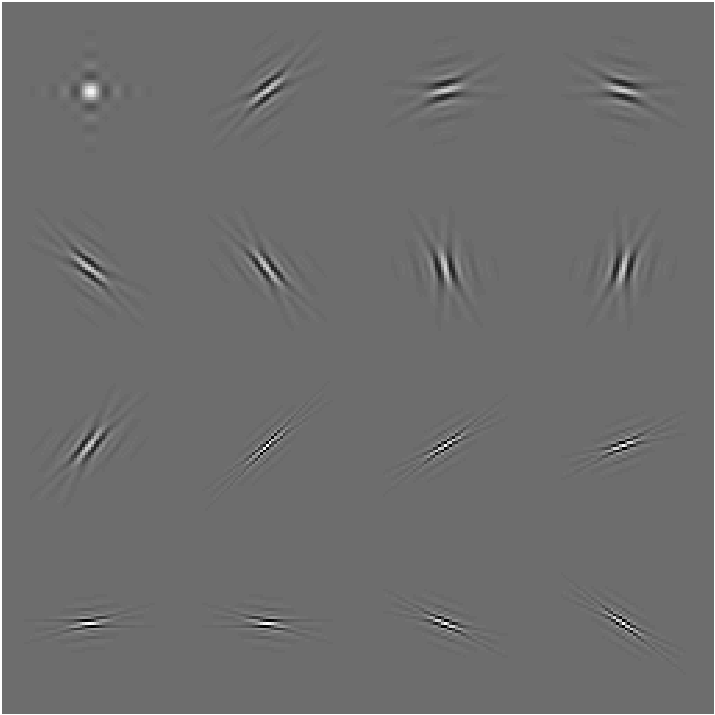
\includegraphics[width=\textwidth]{figures/tree-learn-setup/target.pdf} 
	\caption{Handcrafted target image $\y$}
\end{subfigure}
\begin{subfigure}[b]{0.325\textwidth}\centering
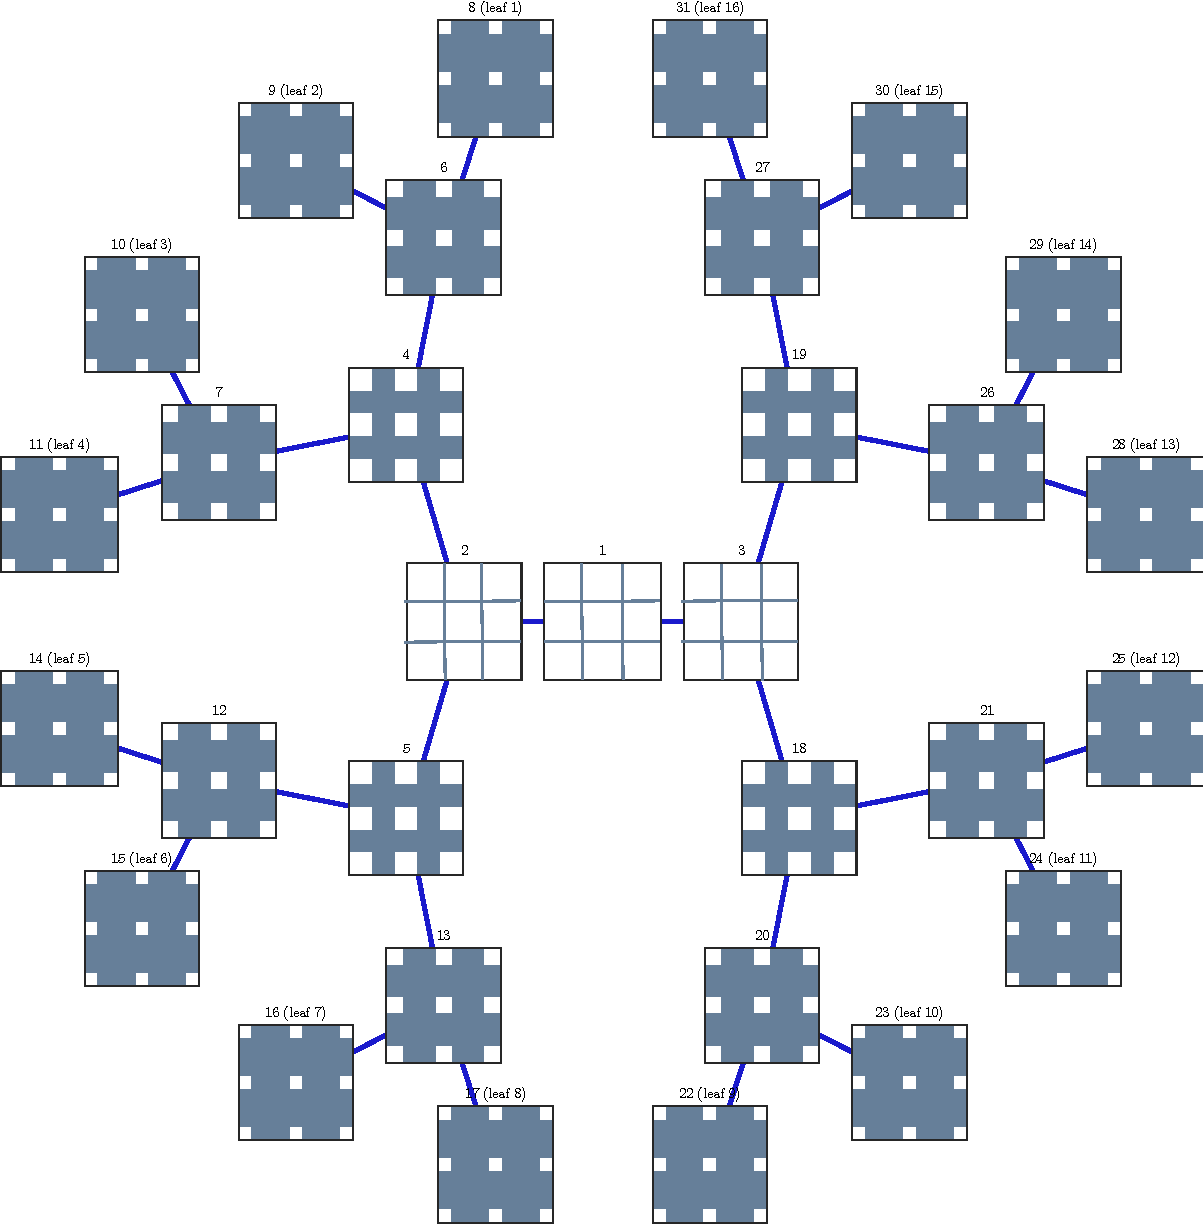
\includegraphics[width=1\textwidth]{figures/tree-learn-setup/xp_learnsupp256_curvelet_decomp3[tree-binary_dpth4]_supp-generic3x3_[fixed-supports]_tree.pdf}
	\caption{Learned tree defining $\D$}
\end{subfigure}
\begin{subfigure}[b]{0.325\textwidth}\centering
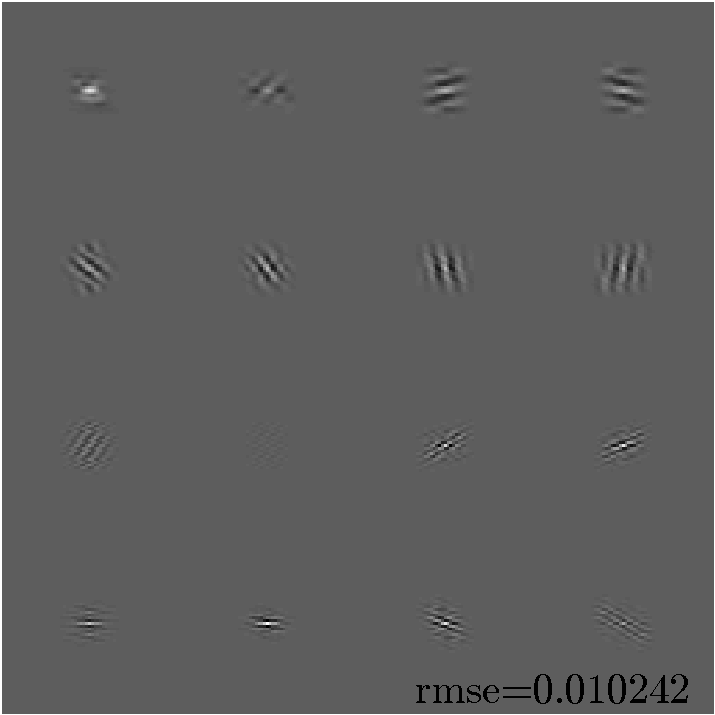
\includegraphics[width=1\textwidth]{figures/tree-learn-setup/xp_learnsupp256_curvelet_decomp3[tree-binary_dpth4]_supp-generic3x3_[fixed-supports]_approx.pdf}
	\caption{Approximation $\D\x$}
\end{subfigure}
\caption{Example of PALMTREE solution. Supports are fixed on a simple binary tree. Codes $\x$ are handcrafted Diracs that exactly match the locations of atoms in $\y$.}\label{fig_exple_fixed_tree}
\end{figure}

\noindent
In fact, without the sparse coding step, \ac{PALMTREE} is limited to images like the one in \cref{fig_exple_fixed_tree}, where the atoms are well separated and located. Therefore, no “real world” images.

\FloatBarrier
\section{Objectives of the present work}

The objective of this work is to study a solution for overcoming the “fixed support” drawback discussed above. To this end, the strategy decided on is to include the support of the atoms as unknowns in the optimization problem.

\begin{figure}[!ht]\centering
\begin{subfigure}[b]{0.32\textwidth}\centering
	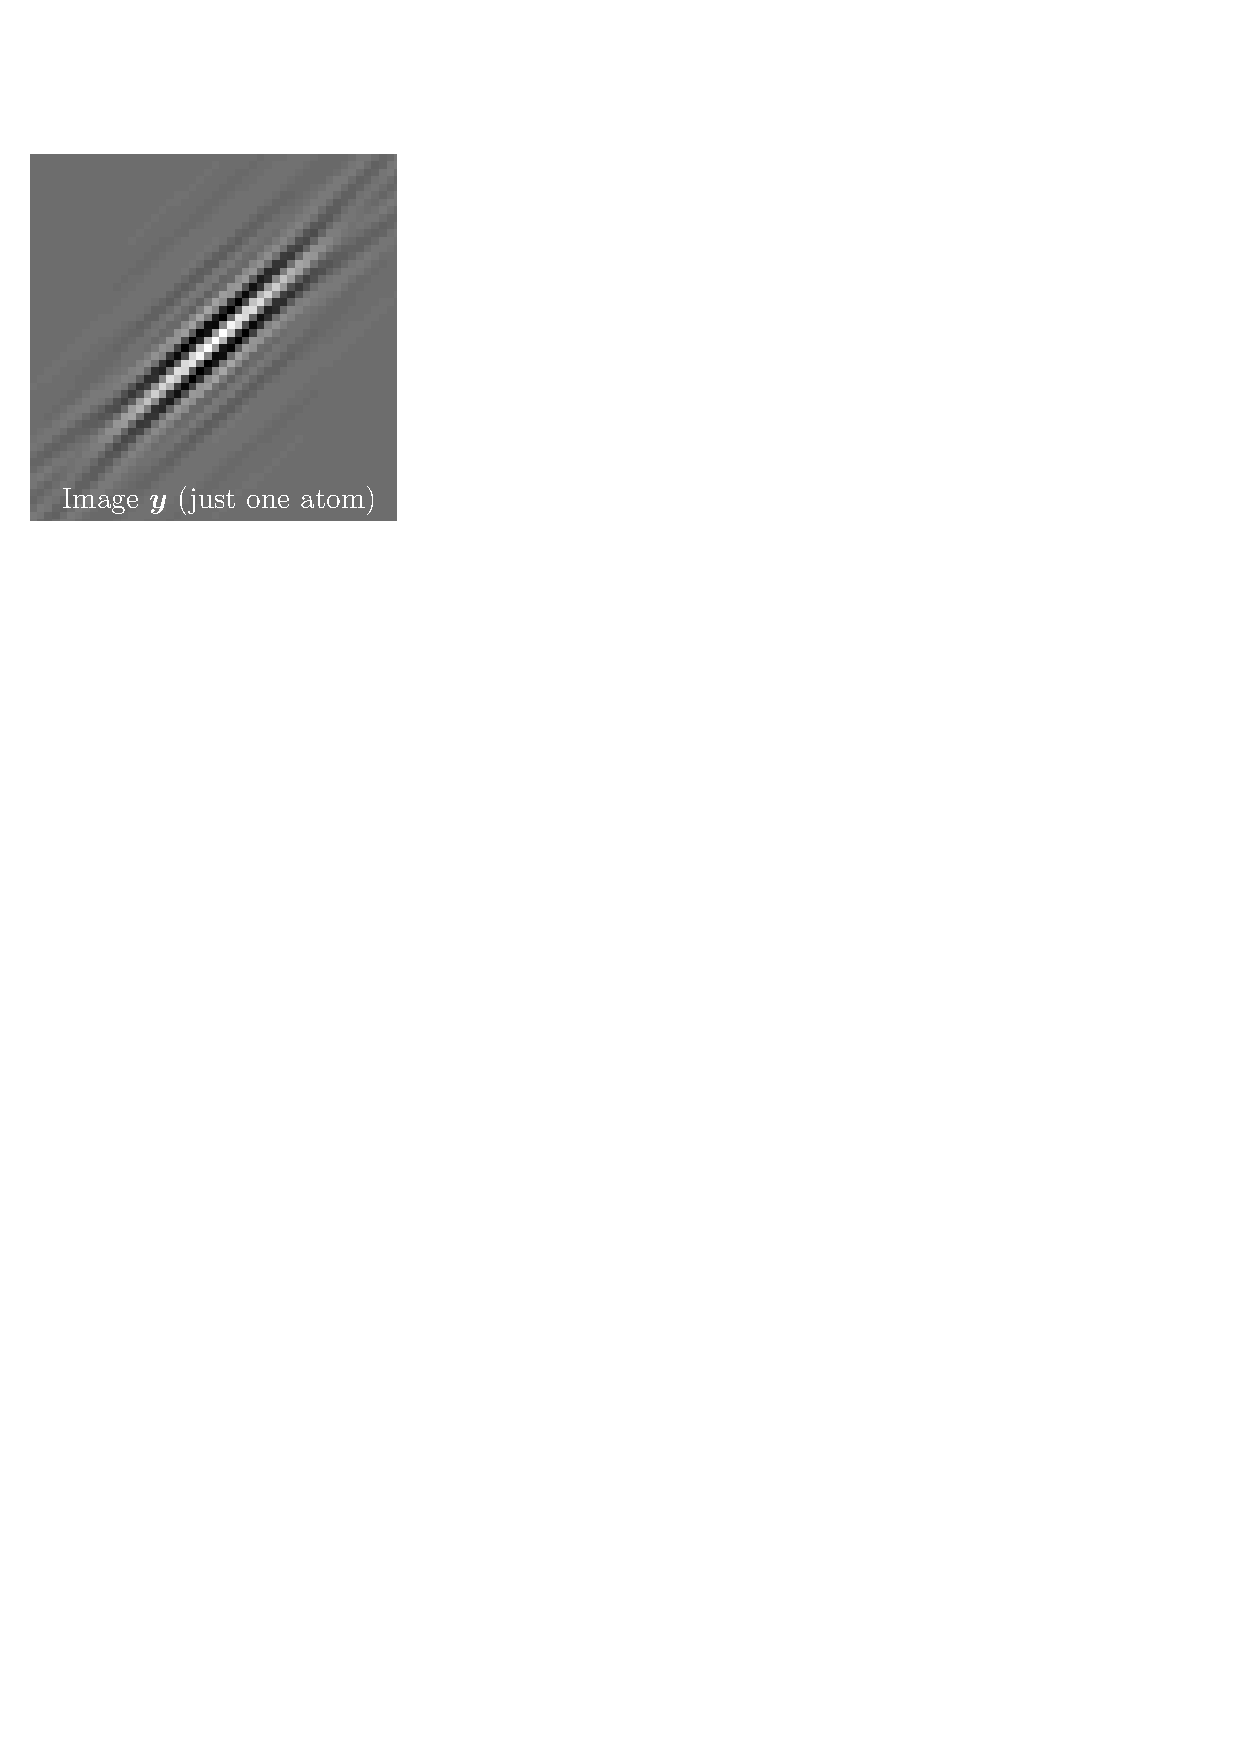
\includegraphics[width=\textwidth]{figures/manual-better-support/target.pdf}
	\caption{Target made out of a curvelet}\label{fig_fixed_vs_expected-target}
\end{subfigure}
\begin{subfigure}[b]{0.32\textwidth}\centering
	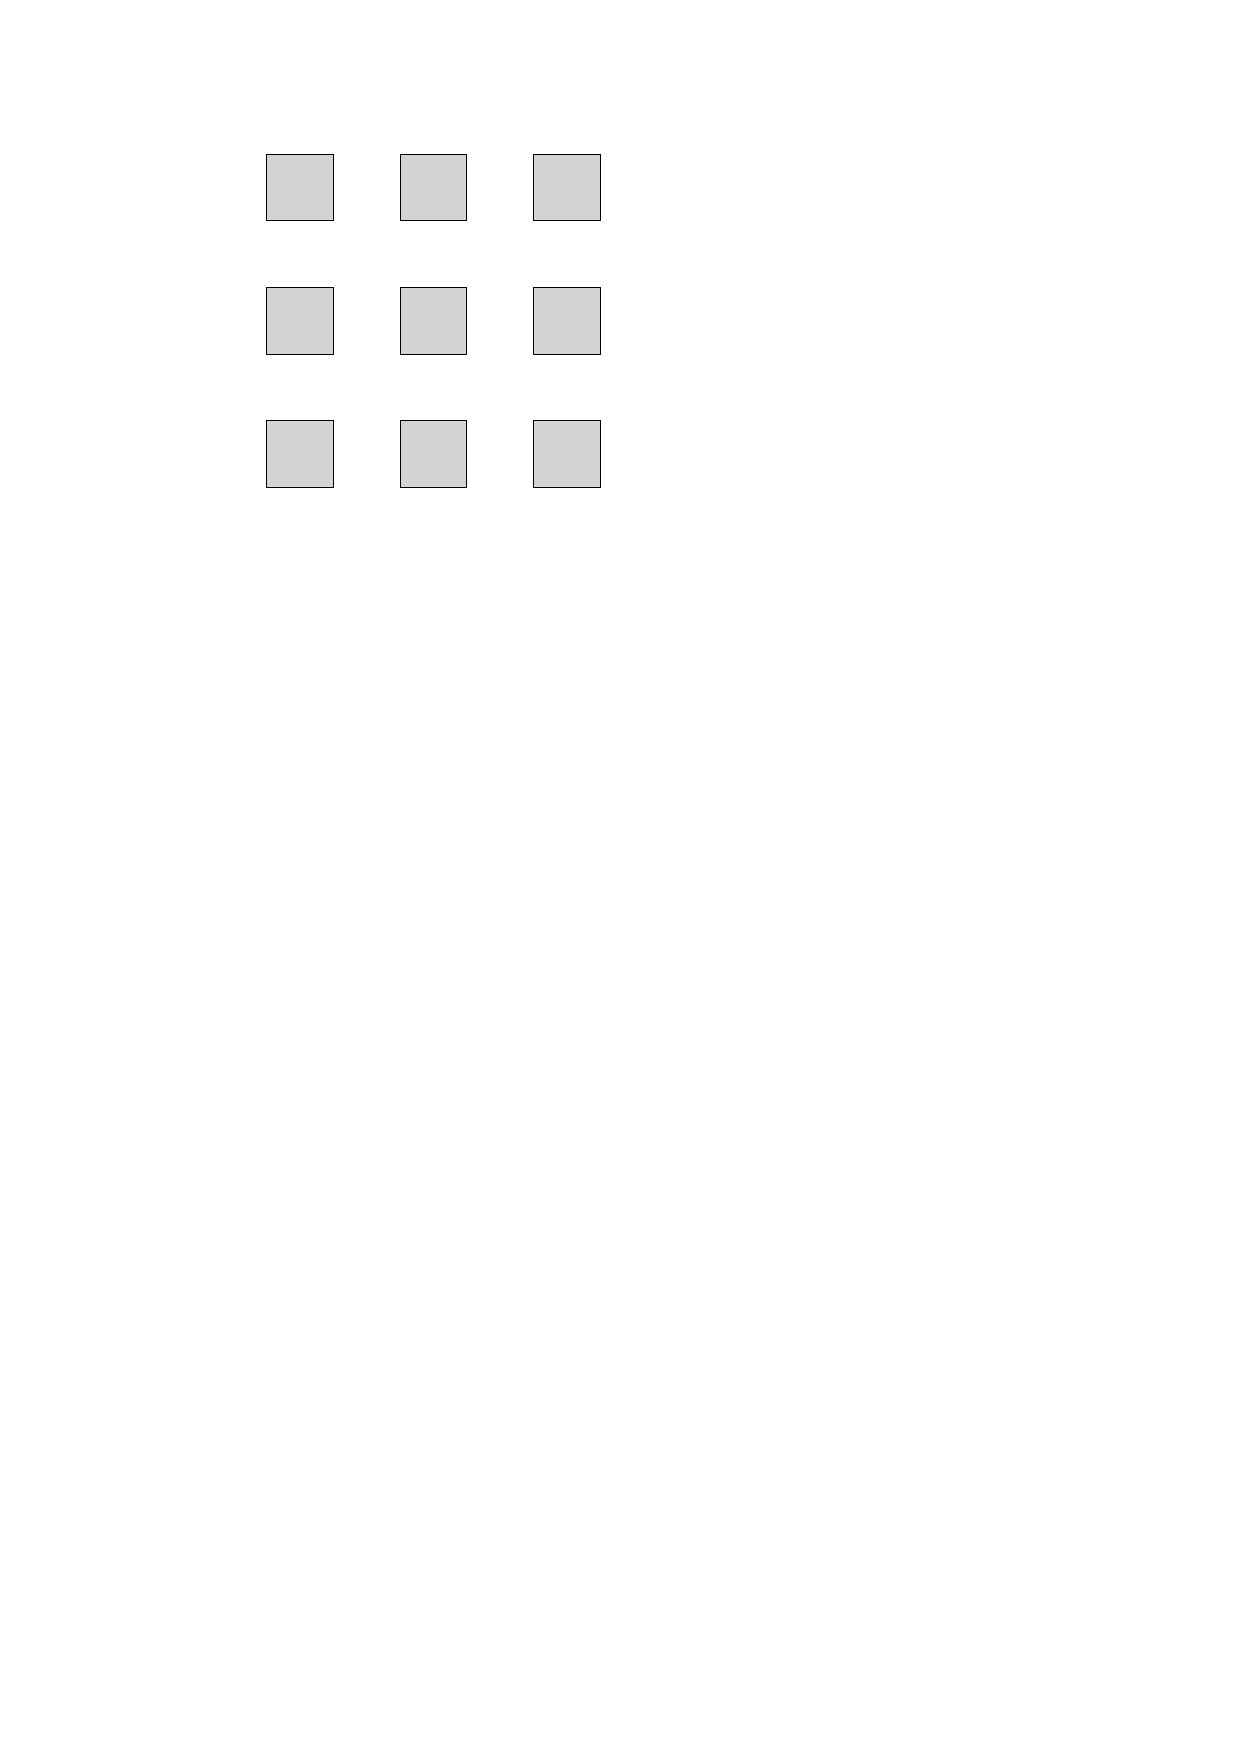
\includegraphics[width=0.5\textwidth]{figures/manual-better-support/support.pdf}
	\caption{Generic support} \label{fig_fixed_vs_expected-generic}
\end{subfigure}
\begin{subfigure}[b]{0.32\textwidth}\centering
	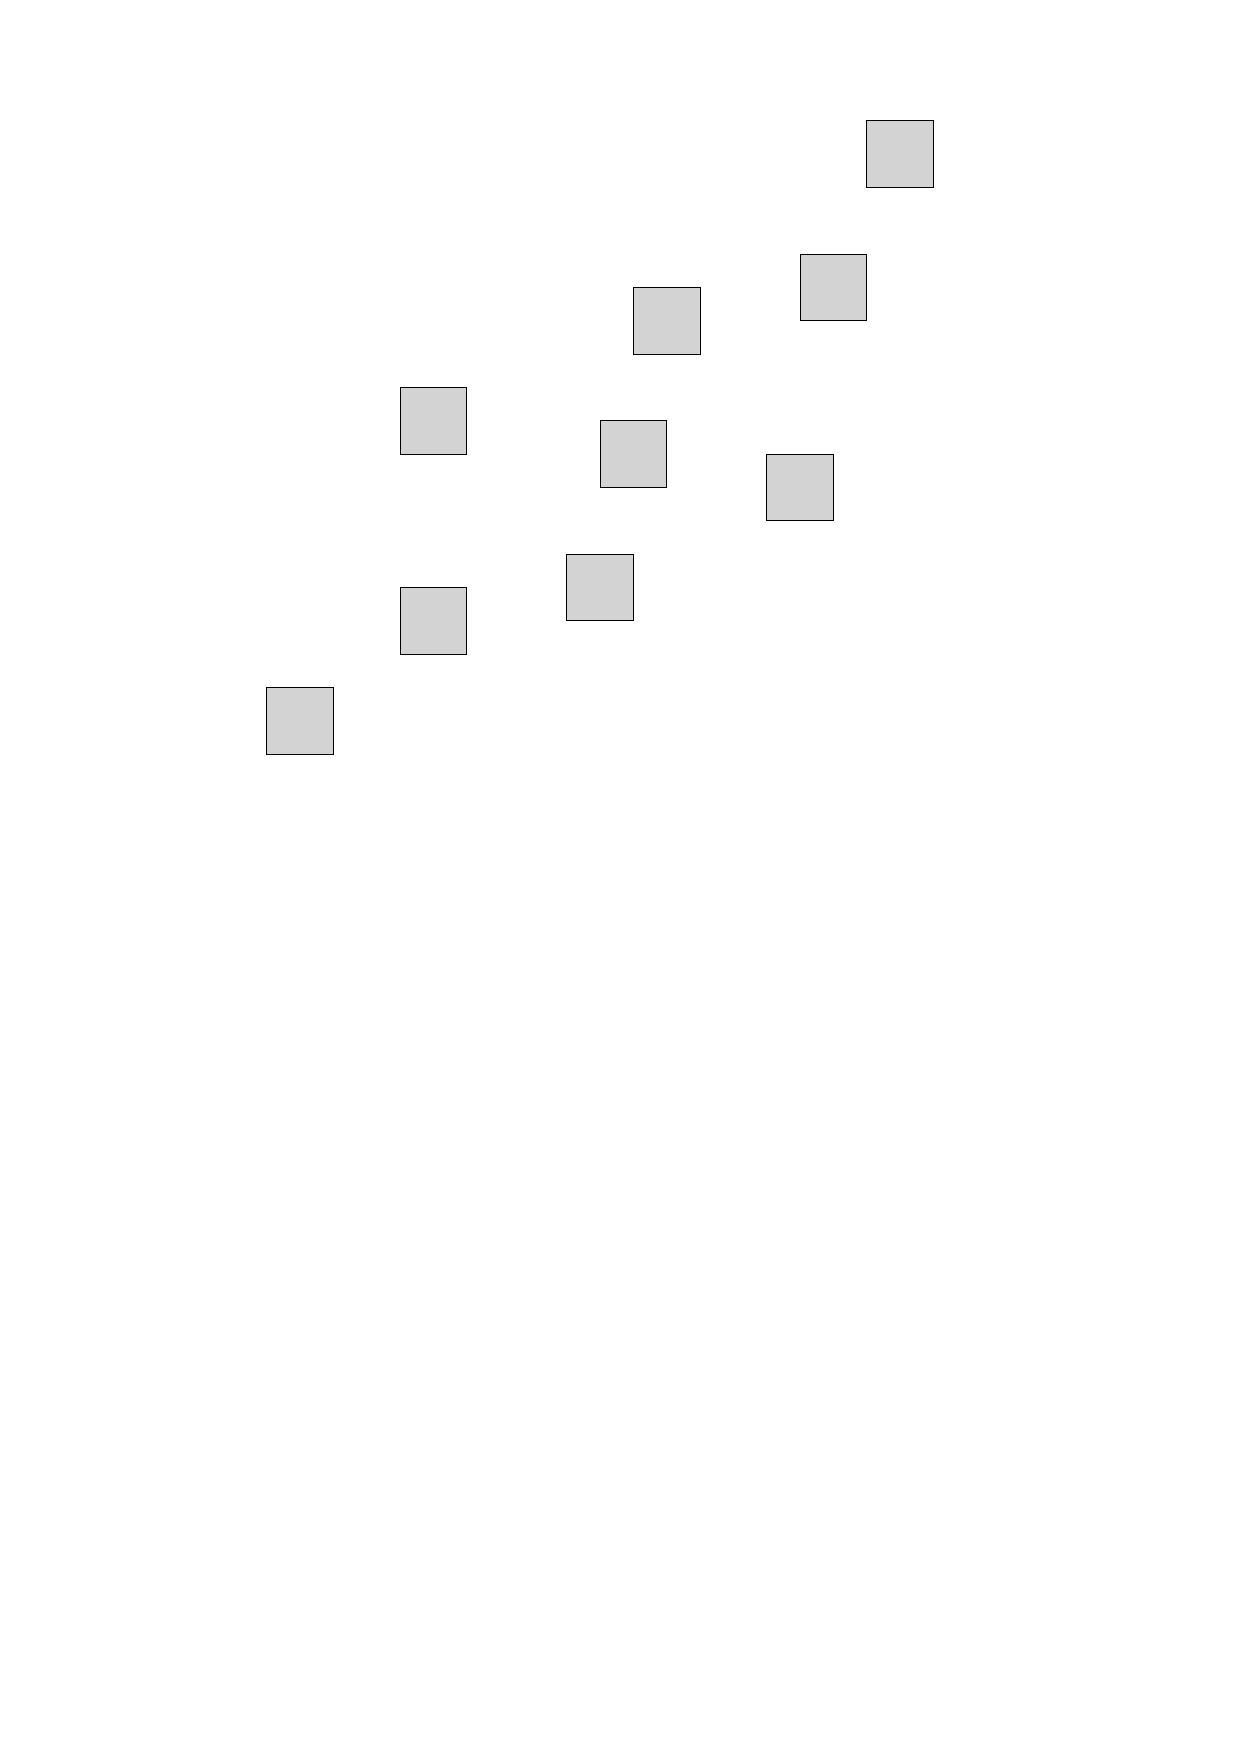
\includegraphics[width=\textwidth]{figures/manual-better-support/support-better.pdf}
	\caption{Expected support} \label{fig_fixed_vs_expected-expected}
\end{subfigure}
\caption{Generic versus expected supports. (b) locations of the support elements for one edge of the tree. (c) a handcrafted support that is expected to provide better results as it follows the general direction of the curvelet.}\label{fig_fixed_vs_expected}
\end{figure}

\noindent
The rationale is that this could enable the support to adapt for specific atoms. An illustration is given in \cref{fig_fixed_vs_expected} where a fixed support is compared to what is an expected solution for an “adaptive” support. In \Cref{fig_fixed_vs_expected-expected}, the support is shaped to better match the target atom of \cref{fig_fixed_vs_expected-target}. \Cref{fig_xp_fixed_vs_expected} experimentally confirms this assumption: after switching $\s^4$ from a generic support to a handmade support that follows the general direction of $\y$ (\cref{fig_fixed_vs_expected-target}), the RMSE\footnotemark[1] is decreased by 16\% (lower is better), which is confirmed by the visual improvement of \cref{fig_xp_fixed_vs_expected_approx2} over \cref{fig_xp_fixed_vs_expected_approx1}.


\footnotetext[1]{Let $\y^1$ and $\y^2 \in \R^N$; the Root Mean Square Error is defined by  \begin{equation*}\text{RMSE}(\y^1,\y^2) =  \sqrt{\frac{1}{N} \sum_{i=1}^N (y^1_i - y^2_i)^2}\end{equation*}}

\begin{figure}[!ht]\centering
\begin{subfigure}[b]{0.085\textwidth}\centering
	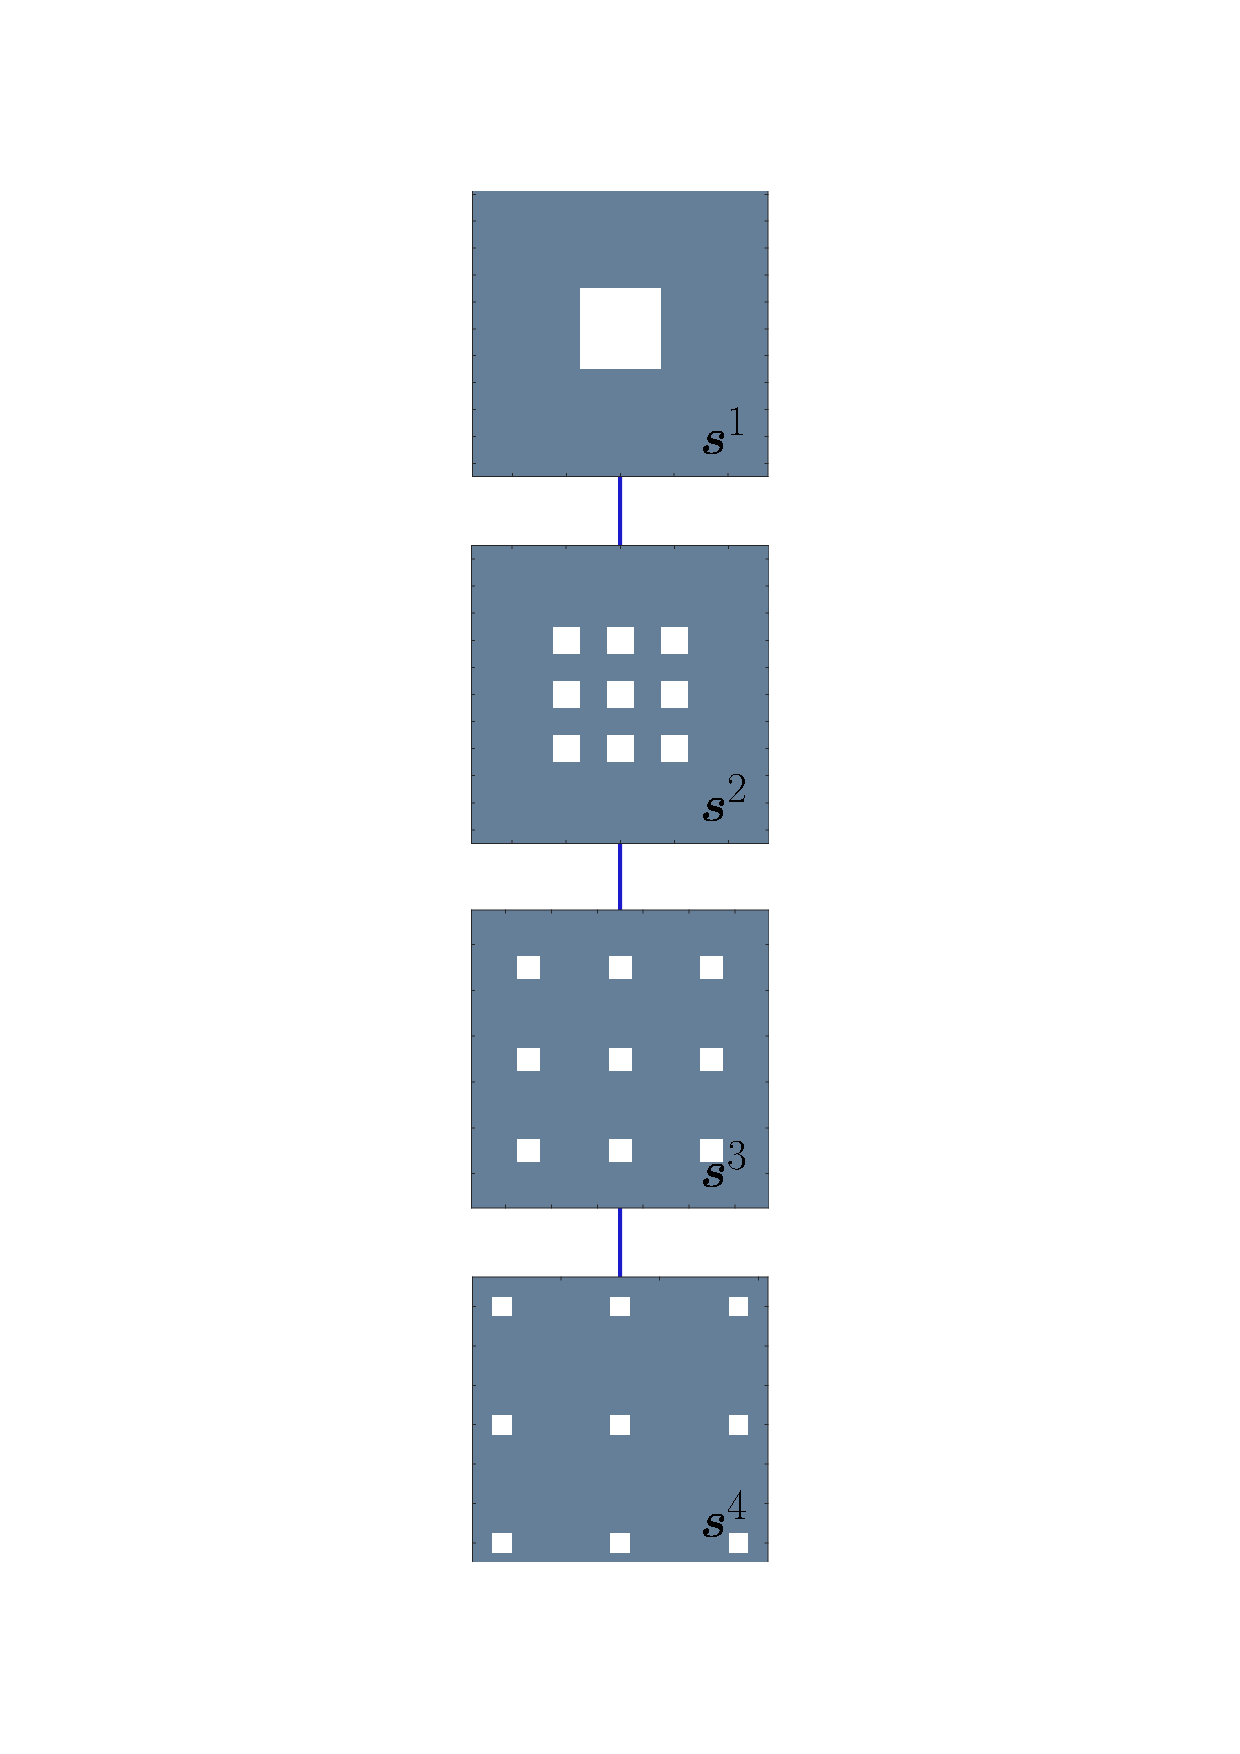
\includegraphics[width=\textwidth]{figures/exple-better-support/tree_classic.pdf}
	\caption{}
\end{subfigure}
\begin{subfigure}[b]{0.39\textwidth}\centering
	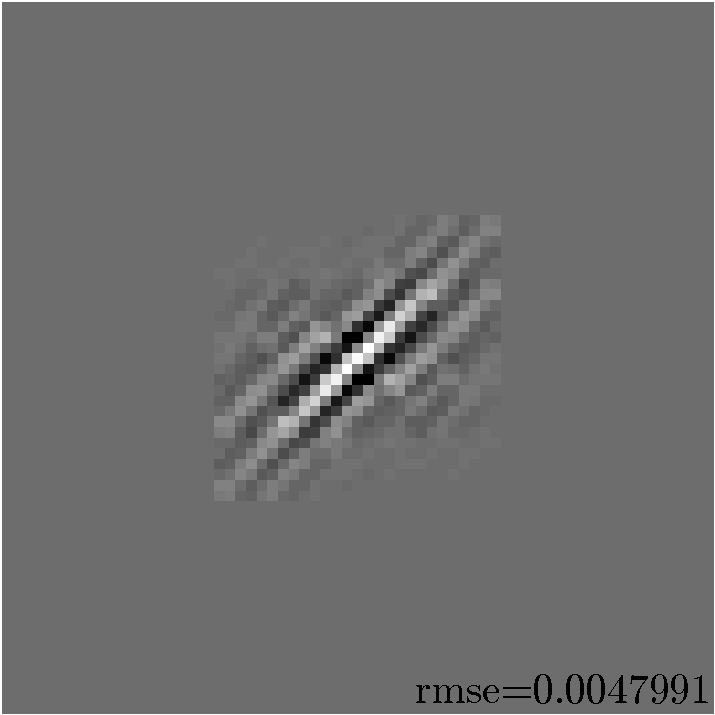
\includegraphics[width=\textwidth]{figures/exple-better-support/xp_128x128_sc2_angl1_K3_S3_node4classic_approx.pdf}
	\caption{$\D\x$ with generic supports}\label{fig_xp_fixed_vs_expected_approx1}
\end{subfigure}
\begin{subfigure}[b]{0.085\textwidth}\centering
	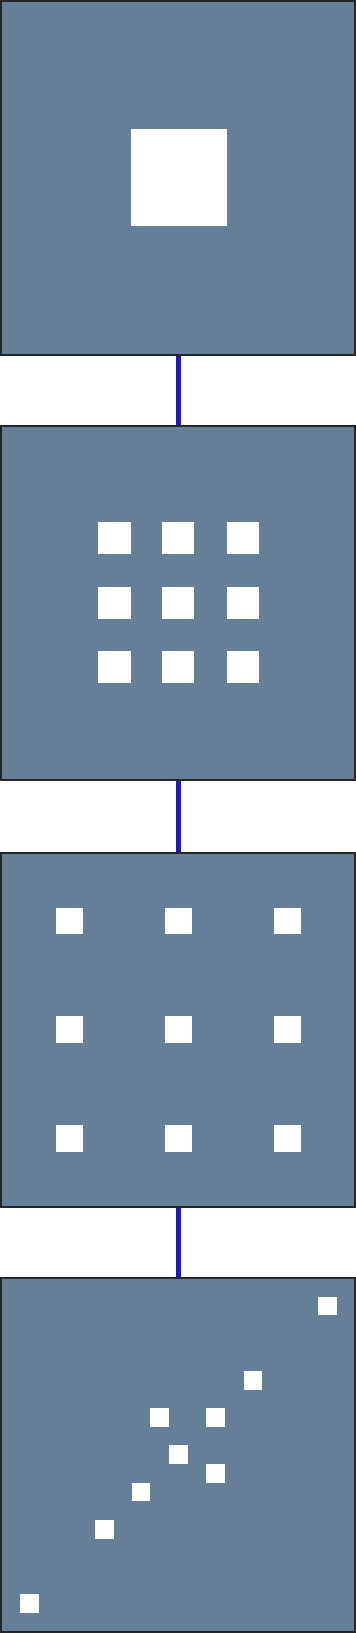
\includegraphics[width=\textwidth]{figures/exple-better-support/tree_expected.pdf}
	\caption{}
\end{subfigure}
\begin{subfigure}[b]{0.39\textwidth}\centering
	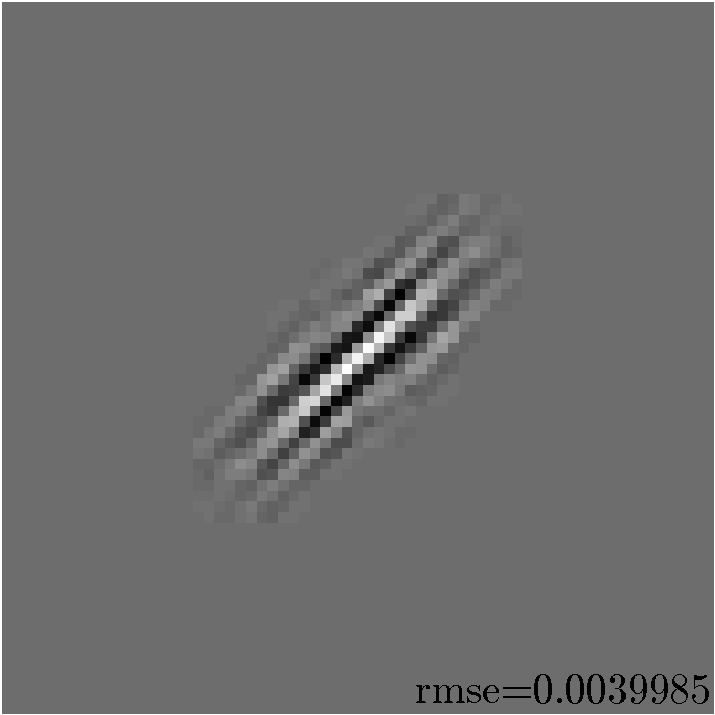
\includegraphics[width=\textwidth]{figures/exple-better-support/xp_128x128_sc2_angl1_K3_S3_node4expected_approx.pdf}
	\caption{$\D\x$ with handcrafted $\s^4$}\label{fig_xp_fixed_vs_expected_approx2}
\end{subfigure}
\caption{Visual enhancement when adapting a support.}\label{fig_xp_fixed_vs_expected}
\end{figure}




\chapter{Experiments}

In the previous chapter, we studied the convolutional tree model proposed in \cite{chabiron_optimization_2016} as an alternative to the slow unstructured dictionaries produced by \ac{KSVD}. The associated algorithm, PALMTREE, yields encouraging results but is limited by the fact that some parameters of the model must be chosen by hand (design of the tree, shape of the supports). Eventually, we proposed in this work to make the supports “adaptative”, i.e. learning them during the optimization process.

\noindent
This chapter reviews our attempts for learning the supports within PALMTREE. More specifically, we identified and studied three sub-problems that are presented in the three next sections: 
\begin{enumerate}[label=--,noitemsep,nolistsep]
	\item \emph{How to decide on which elements to add?} For this problem, we propose a solution based on the gradient and inspired from the \acs{OMP} algorithm;
	\item \emph{How to solve for one branch?} For this sub-problem, we propose a multi-adding scheme with a partial PALMTREE solution for each \acs{OMP} iteration;
	\item \emph{How to solve for a tree?} For this sub-problem, which is actually a problem on its own, we compare several strategies together with the introduction of a prior parameter for localizing the atoms.
\end{enumerate}


\section{Choice of the element to add}

We proposed in this work to learn the supports along with the kernels. In this section, we study the possibility of using the gradient defined in \cref{eq_gradient} (\cpageref{eq_gradient}) for locating the best support element (not already in the support) that we might then add. 

\noindent
The motivation is that the direction of largest gradient coefficient indicates the direction of the strongest local decrease of the objective function; assuming that this direction wasn't in the support, incorporating it will lead to a (locally) better solution.

\noindent 
After defining the experimental setup for testing the gradient as a mean for adding a support element, we study the computability of the gradient. We then check that the position of largest gradient direction leads to a good support element, comparing the gradient greatest directions to an empirical ground truth. We eventually notice that the greatest gradient direction can be used for adding a support element before the convergence of PALMTREE.

\subsection{Experimental setup}
Every experiment in the first part of this chapter uses a fixed single-branch tree of depth 4 associated with $\y$, $\h^e$, $\s^e$ and $\x^e$ of size $128 \times 128$. The figures only display the central $64 \times 64$ pixels as shown in \cref{fig_xp_explain}.

\begin{figure}[!ht]\centering
\begin{subfigure}[b]{0.32\textwidth}\centering
	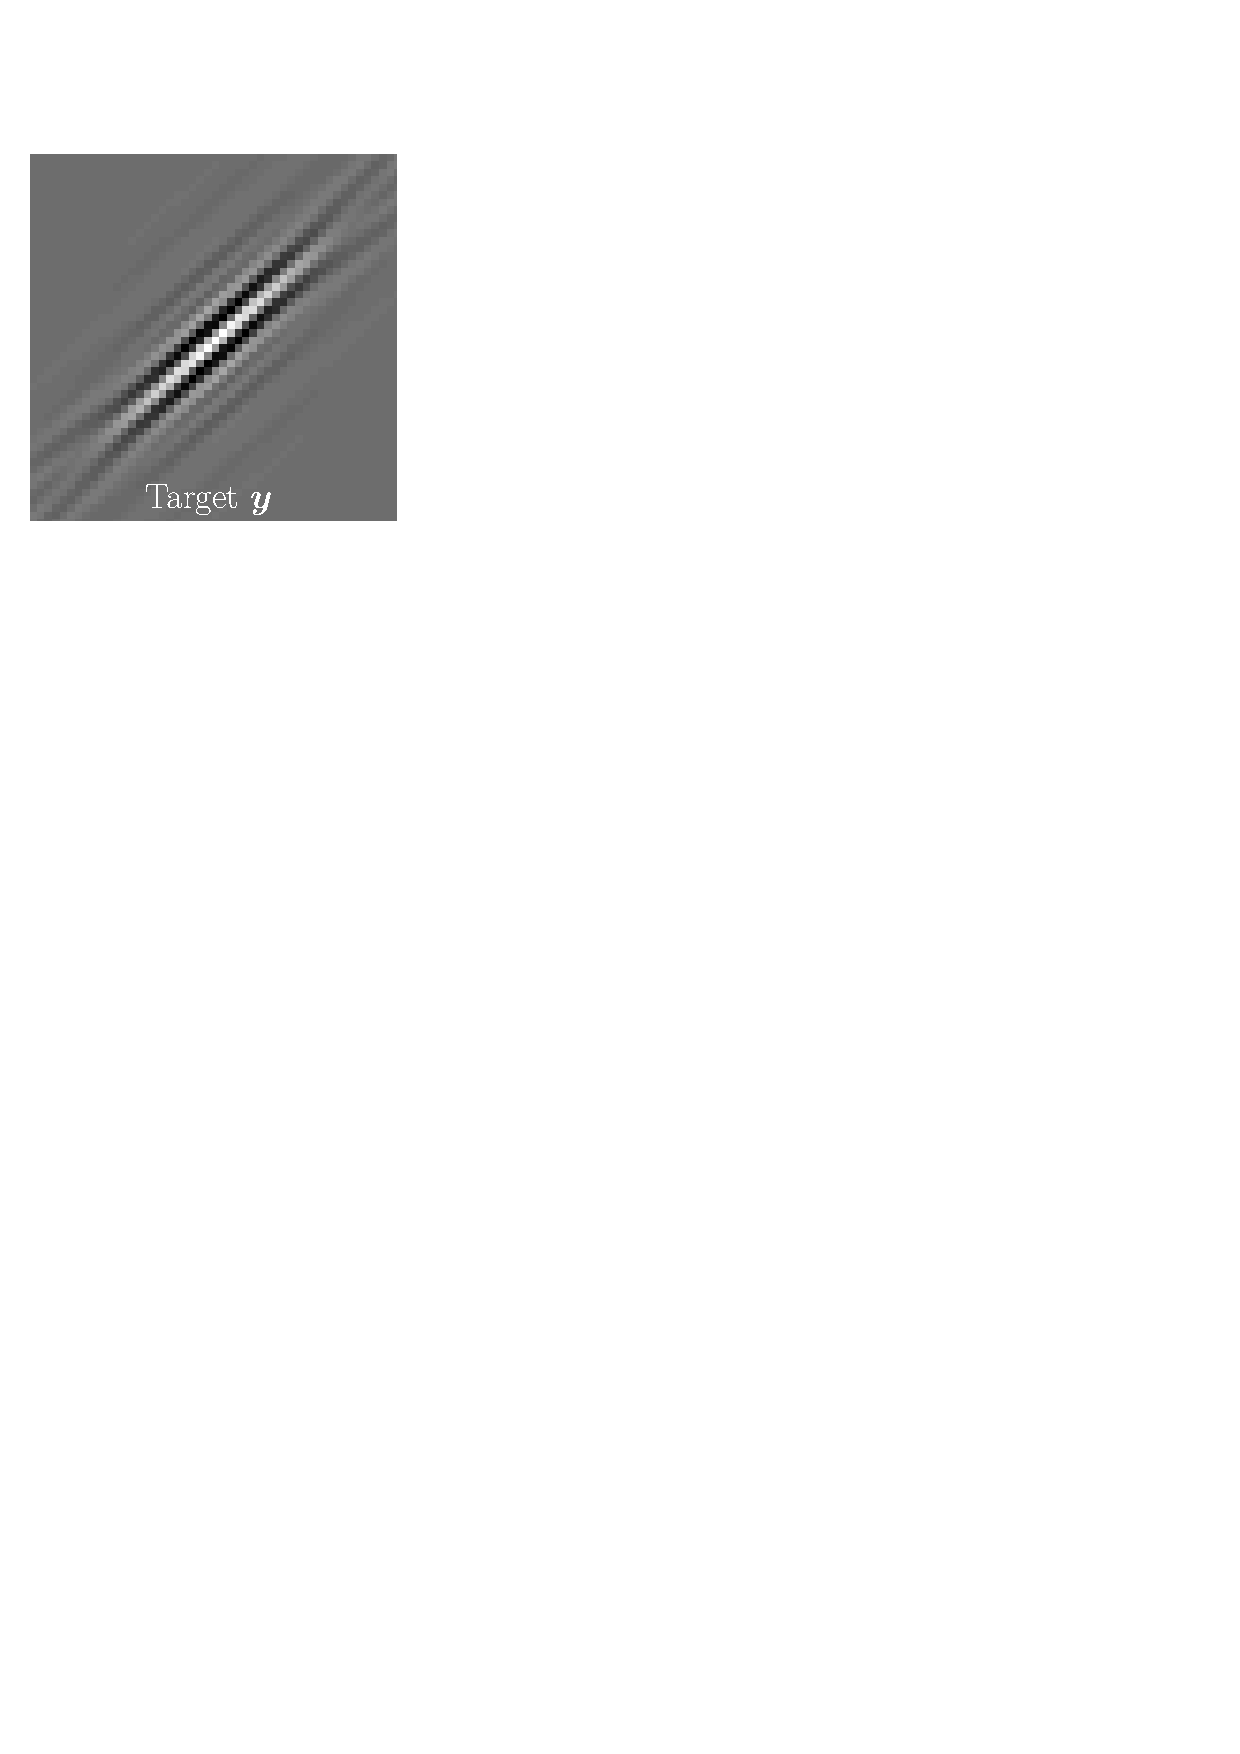
\includegraphics[width=0.9\textwidth]{figures/xp_explain/target.pdf}
	\caption{}
\end{subfigure}
\begin{subfigure}[b]{0.32\textwidth}\centering
	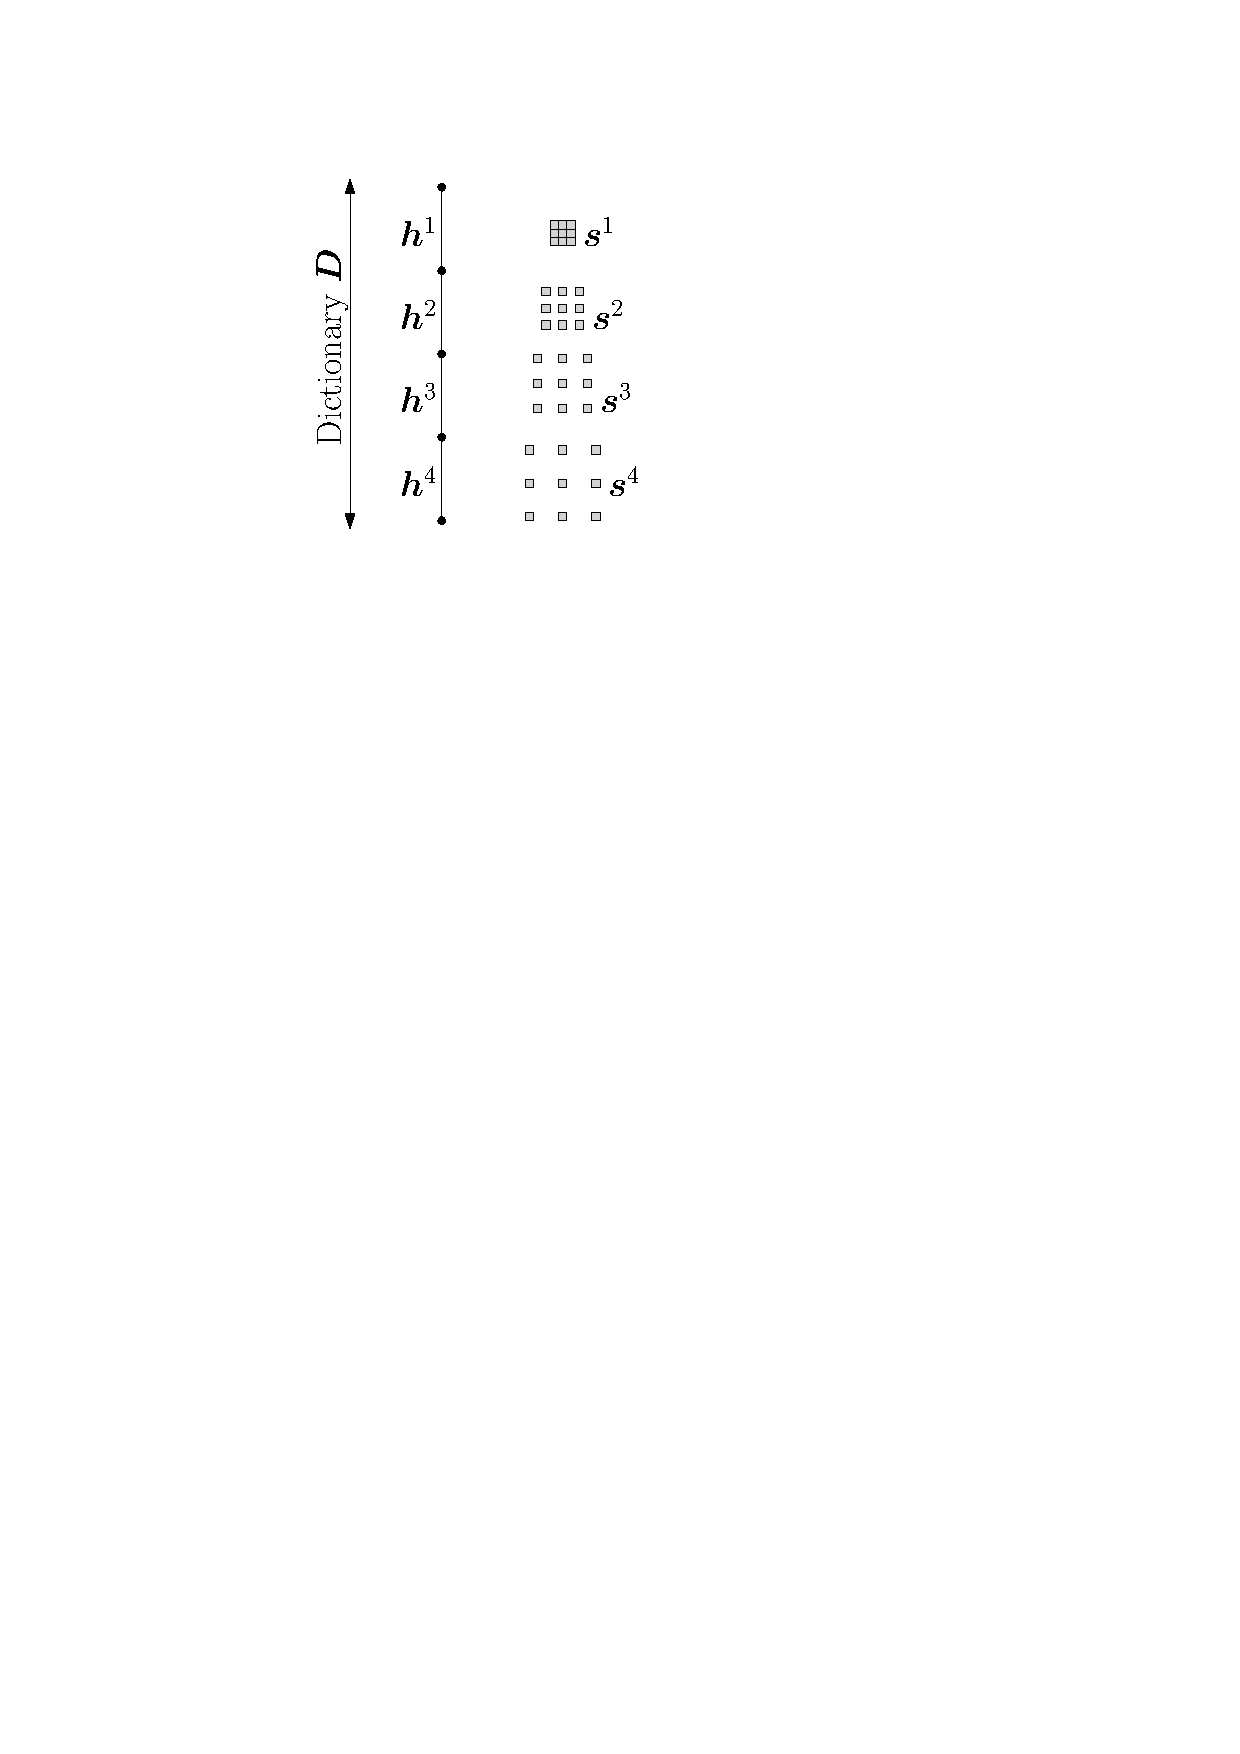
\includegraphics[width=0.9\textwidth]{figures/xp_explain/dictionary.pdf}
	\caption{}
\end{subfigure}
\begin{subfigure}[b]{0.32\textwidth}\centering
	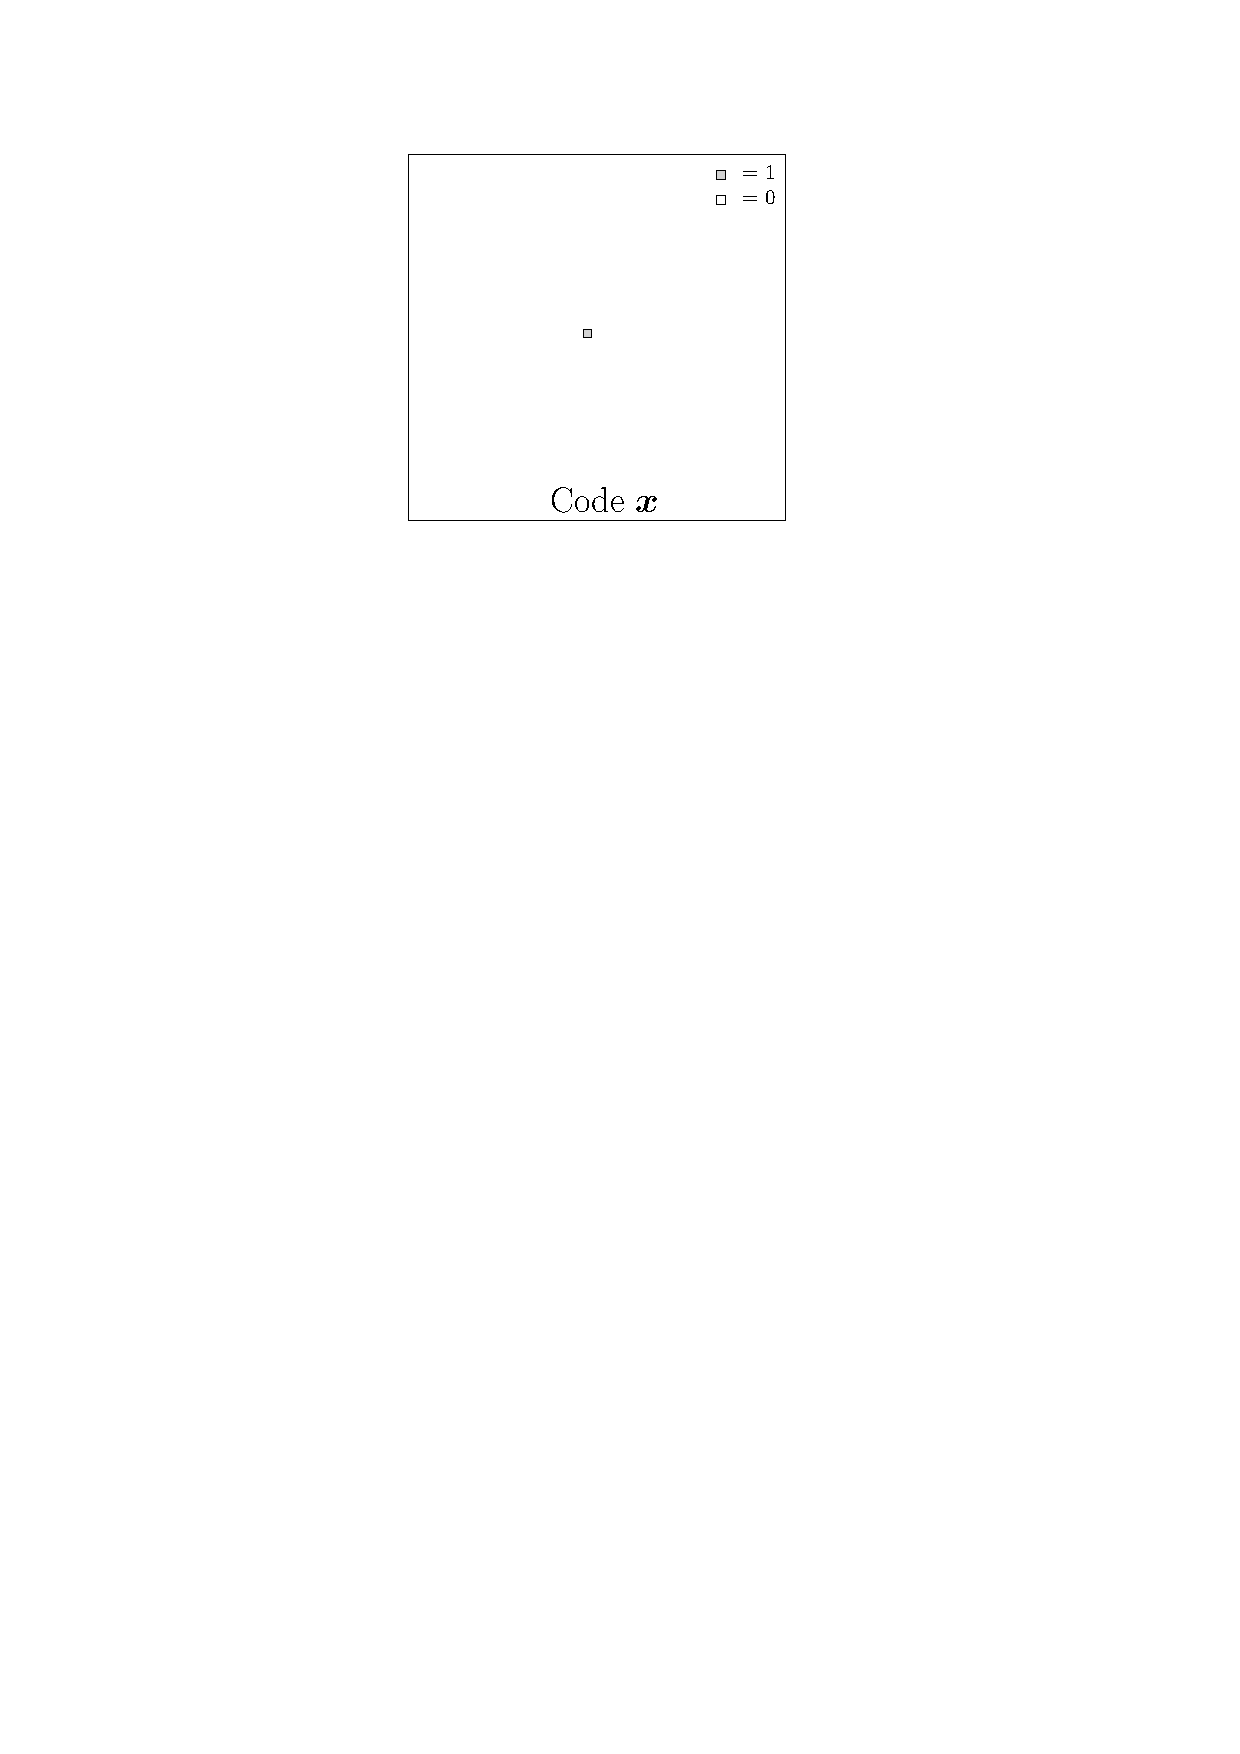
\includegraphics[width=0.9\textwidth]{figures/xp_explain/code.pdf}
	\caption{}
\end{subfigure}
\caption{Experimental setup. The experiments use one image $\y$, one dictionary $\D$ (formed by $\T$, $(\s^e)_{e \in \E}$, $(\h^e)_{e \in \E}$) and one code $\x$. The parameters $\y$, $\x$, $\T$, $(\s^e)_{e \in \E}$ are given and $(\h^e)_{e \in \E}$ is estimated from the observed image $\y$.}\label{fig_xp_explain}
\end{figure}

\noindent
In the following experiments, the dictionary associated with this convolutional tree is 
\begin{equation*}\D = \h^1 * \h^2 * \h^3 * \h^4.\end{equation*}

\subsection{Using the gradient for choosing the element to add}

The Orthogonal Matching Pursuit (\ac{OMP}, detailed in \cref{alg_omp}) chooses at \cref{alg_omp_pick_correlation} which component $\x_i$ should be “turned on” at each iteration, finding the atom $\d_i$ that has the greatest correlation with the residual $\Res = \D\x - \y$, i.e.,
\begin{equation*} i = \underset{j}{\argmax} ~ | \D^T \Res |_j \end{equation*}
which is litterally the same as computing the gradient $\nabla \Phi(\x)$ with $\Phi(\x) = \lVert \D\x - \y \rVert^2$.

\begin{algorithm}[!ht]
    \caption{Orthogonal Matching Pursuit (OMP) algorithm for standard sparse approximation}\label{alg_omp}
  \begin{algorithmic}[1]
    \Input signal $\y$ of dimension $N$, dictionary of dimension $N \times K$ with $K \gg N$
    \Output A $k$-sparse code $\x$ of dimension $K$
    \State \textbf{Initialization} $S=\{\}$
    \For{$i = 1,\dots,k$}
      \State $j =  \underset{j = 1,\dots,K}{\argmax}~| \nabla \Phi(\x)_j |$\label{alg_omp_pick_correlation}\Comment{find atom with max. correlation with residual $\Res$}
      \State $S = S \cup \{j\}$
      \State $\x = \underset{\text{supp}(\x) \subset S}{\argmin} \Phi(\x)$
    \EndFor
  \end{algorithmic}
\end{algorithm}

Our idea is to use the same principle when adding elements to supports $(\s^e)_{e \in \E}$: add a new element to one of the supports between two minimizations of the \ac{PALMTREE} algorithm, using the largest gradient component.

\begin{algorithm}[!ht]
    \caption{\ac{OMP} algorithm using \ac{PALMTREE} (OMP-PALMTREE)}\label{alg_omppalmtree}
  \begin{algorithmic}[1]
    \Input signal $\y$ of dimension $N$, kernel sparsity level Q (defined in \cref{eq_Q}), dictionary of dimension $N \times K$ with $K = |\L| \cdot N$ and $K \gg N$
    \Output The Q-sparse kernel supports $\s$
    \State \textbf{Initialization} Initialize the supports $\s^e$ with Diracs (at the beginning, the kernel sparsity level is $|\E|$)
    \For{$i = |\E|+1,\dots,Q$}
      \State $(e,p) = \underset{(e,p) \in \E \times \P}{\argmax}~ |\nabla \Phi_{\h^e}(\h)_p|$\Comment{Choose support $s^e$ and location $p$}\label{alg_omppalmtree_find}
      \State $\s^e_p = 1$
      \State $\h = \underset{\h^e \in \Dspace^e}{\argmin}~ \Phi(\h)$ \Comment{Solve \eqref{eq_ftl} using \ac{PALMTREE}}\label{alg_omppalmtree_ftl}
    \EndFor
  \end{algorithmic}
\end{algorithm}

\noindent
\Cref{alg_omppalmtree} presents an adaptation of the \ac{OMP} algorithm for the \gls{treemodel}, denoted as OMP-PALMTREE.

\noindent
However, three questions arose when designing this new “meta” algorithm:
\begin{enumerate}[label={\alph*)},noitemsep]
	\item At \cref{alg_omppalmtree_find}, is it actually correct to choose the element to be added using a strictly local information given by the gradient?
	\item Also, at \cref{alg_omppalmtree_find}, how would we get the “full” gradient (defined in \cref{sec_full_grad} below) while the current gradient is only computed on the points of the support?
	\item Finally, at \cref{alg_omppalmtree_ftl}, is it really necessary to wait for the convergence of \eqref{eq_ftl}?
\end{enumerate}

\noindent
Before answering these questions, we will first review how the “full” gradient is computed and then describe a way to check that the “full” gradient gives a good direction towards a critical point, comparing it with what we call “gain-per-added-point”, detailed in \cref{sec_gain_per_added_point} below. Finally, we will give some thoughts on whether we should wait until \eqref{eq_ftl} converges or if a smaller number of iterations suffice between two iterations of OMP-PALMTREE.


\subsubsection{Computing the “full” gradient}\label{sec_full_grad}
Up to now, the gradient was computed using a convolution based on translations, as mentioned in \cref{sec_palmtree}. This computation takes advantage of the sparsity of each kernel $\h^e$ as well as the fact that the proximal operator is projecting every kernel onto its support, meaning that only a few elements have to be computed. We denote it as the “sparse” gradient.

\noindent
However, the OMP-PALMTREE algorithm requires a gradient defined on every point $p \in \P$. We denote it as the “full” gradient.

\noindent
In order to compute the “full” gradient, we basically chose to use the fast Fourier transform ($\F$), i.e., 
\begin{align*}
	\nabla_{\h^e} \Phi((\h^f)_{f \in \E})&= 2 \F^{-1}(\F(\H^{e})^* \circ \F(\Res))
\end{align*}
with ${}^*$ denoting the adjoint operator, $\circ$ the Hadamard product (point-wise product). The notations $\H^e$ and $\Res$ have been defined in \cref{sec_palmtree}.

\subsubsection{Validation of the “full” gradient}
We had some trouble when trying to compute the gradient on the full kernels $(\h^e)_{e \in \E}$ (not only on the support elements). To ensure that the computed “full” gradient was correct, we compared it to a finite-difference approximation of the gradient, exploiting the fact that
\begin{equation*}\lim_{\epsilon \rightarrow 0} \frac{\Phi((\h^e)_{e \in \E}+\epsilon e_i) - \Phi ((\h^e)_{e \in \E}) }{\epsilon} ~=~ \nabla_i \Phi ((\h^e)_{e \in \E}).\end{equation*}

\begin{figure}[!ht]\centering
\begin{subfigure}[b]{0.30\textwidth}\centering
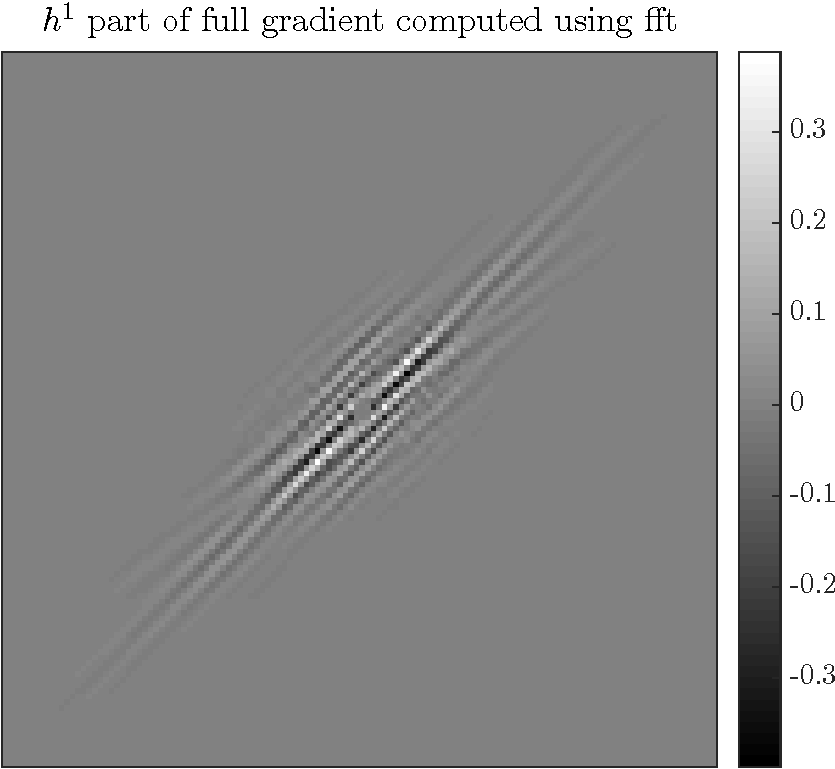
\includegraphics[width=\textwidth]{figures/verif_gradient/gradient.pdf}
\caption{“Full” gradient}\label{fig_verif_gradient-grad}
\end{subfigure}
\begin{subfigure}[b]{0.30\textwidth}\centering
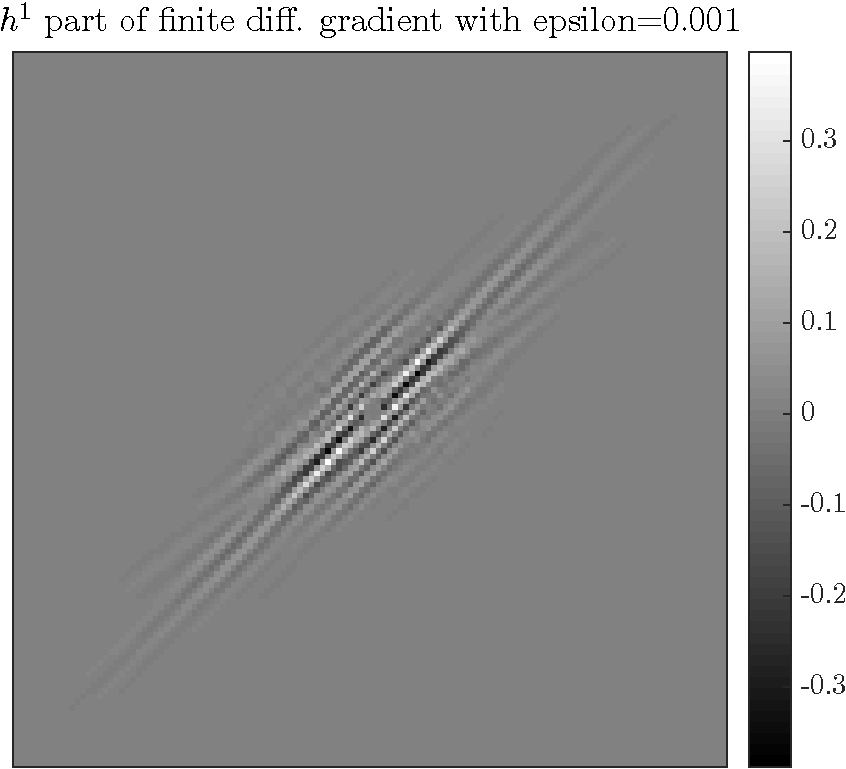
\includegraphics[width=\textwidth]{figures/verif_gradient/finite-diff.pdf}
\caption{Finite-difference}\label{fig_verif_gradient-finite}
\end{subfigure}
\begin{subfigure}[b]{0.35\textwidth}\centering
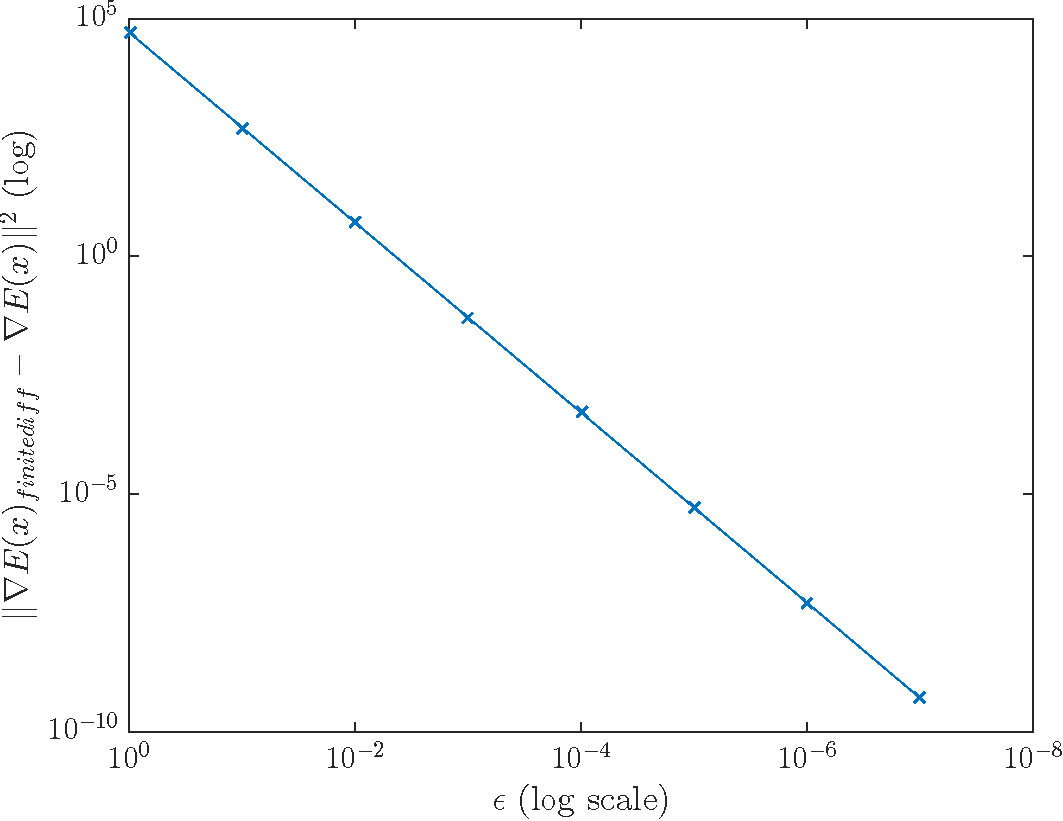
\includegraphics[width=\textwidth]{figures/verif_gradient/finite-diff-vs-grad.pdf}
\caption{Error w.r.t.\@ $\epsilon$}\label{fig_verif_gradient-error}
\end{subfigure}
\caption{Full gradient, its estimation and the error between these two quantities.}\label{fig_verif_gradient}
\end{figure}

\noindent
Figure \ref{fig_verif_gradient} compares the FFT-computed gradient to the finite-difference approximation of the gradient (with $\epsilon=0.001$). \Cref{fig_verif_gradient-grad,fig_verif_gradient-finite} show that the two gradients are visually very close. \Cref{fig_verif_gradient-error} shows that the finite-difference gradient converges to the “full” gradient, which confirms that our “full” gradient implementation is correct.


\subsection{Gain-per-added-point to the support}\label{sec_gain_per_added_point}

We want to check whether the gradient provides relevant information on which elements to add to support. To do so, we compare it with the actual decrease of objective function (namely the \emph{gain-per-added-point}) when a single element is added to the support.

\noindent
In this purpose, we designed \cref{alg_gain_per_added_point} for computing what we call the \emph{gain-per-added-point} matrix, denoted $\g^f$ ($f$ is the edge of the studied support). \Cref{alg_gain_per_added_point} tries every possible point that can be added to one given support $s^f$, quantifies how much the objective function decreases when adding the point and continuing the minimization and finally stores it in the matrix gain-per-added-point.

\begin{algorithm}[!ht]
    \caption{Gain-per-added-point $\g^f$ for the support $\s^f$}\label{alg_gain_per_added_point}
  \begin{algorithmic}[1]
    \Input One chosen edge $f \in \E$ and a tree $\T$, supports $\s$ and kernels $\h$
    \Output $\g^f$, the gain per added point for support $\s^f$
    \State $\h^{\text{start}} = \underset{\h}{\argmin}~ \Phi (\h)$ \quad s.t.~$\h^e \in \Dspace^e$ \quad $\forall e \in \E$ \Comment{common starting point}
    \For{each point $p$ of $\P$}
    	\State $\s^f_p = 1$ \Comment{add element to support}
    	\State Set $\h = \h^{\text{start}}$
    	\State $\g^f_p = \Phi(\h^{\text{start}}) - \underset{\h^e \in \Dspace^e}{\min}~ \Phi (\h)$ \quad $\forall e \in \E$ \Comment{Compute gain for the considered point}
    	\State $\s^f_p = 0$ \Comment{remove element from support}
    \EndFor
  \end{algorithmic}
\end{algorithm}

\begin{figure}[!ht]\centering
	\begin{subfigure}[b]{0.30\textwidth}\centering
	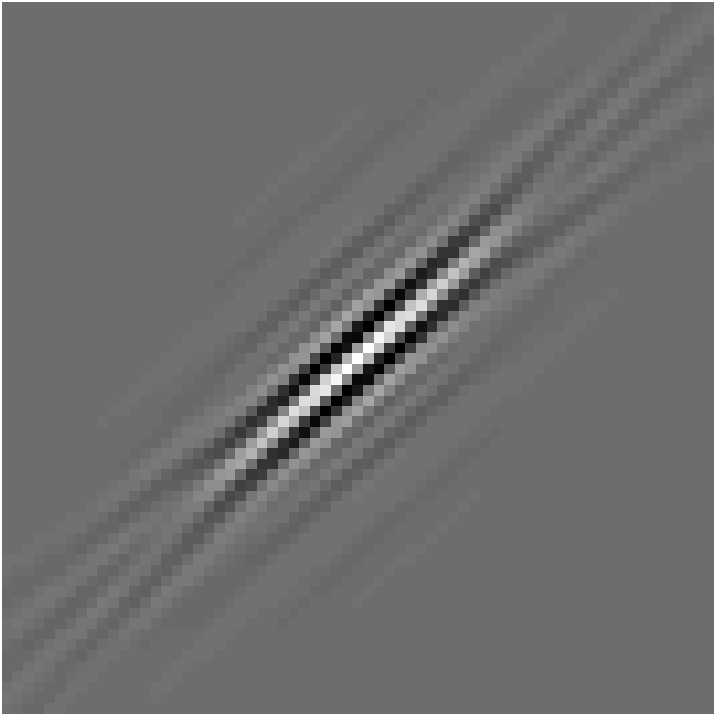
\includegraphics[width=\linewidth]{figures/xp/n4/xp_128x128_sc2_angl1_K3_S3_node4_target.pdf}
	\caption{Target $\y$} \label{fig_gain_n4-target}
	\end{subfigure}
	\begin{subfigure}[b]{0.34\linewidth}\centering
	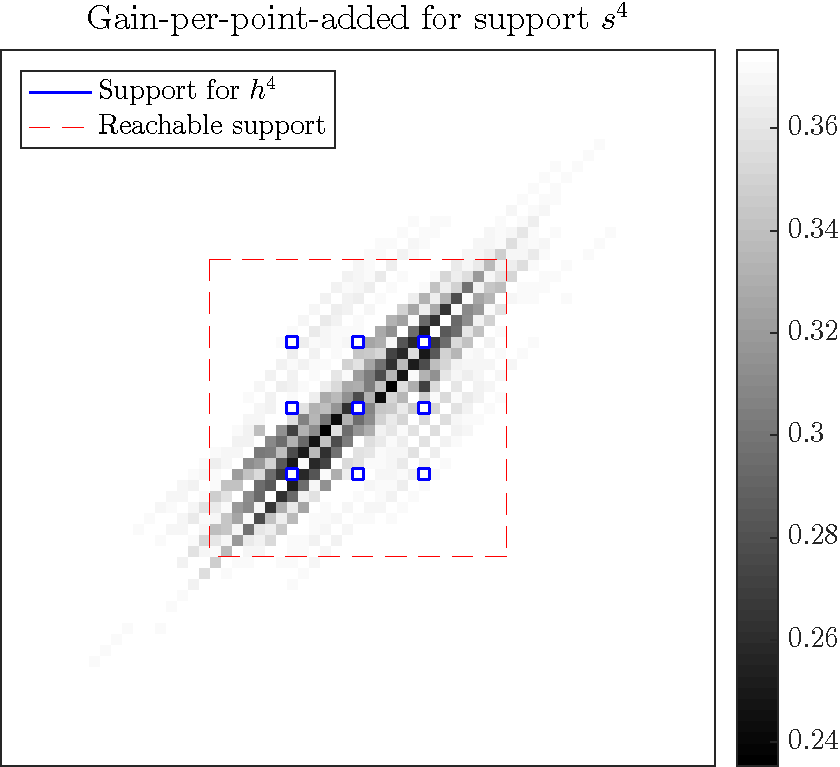
\includegraphics[width=\linewidth]{figures/xp/n4/xp_128x128_sc2_angl1_K3_S3_node4_objmatrix.pdf}
	\caption{Gain-per-added-point for $\s^4$}\label{fig_gain_n4-gain}
	\end{subfigure}
	\begin{subfigure}[b]{0.34\linewidth}\centering
	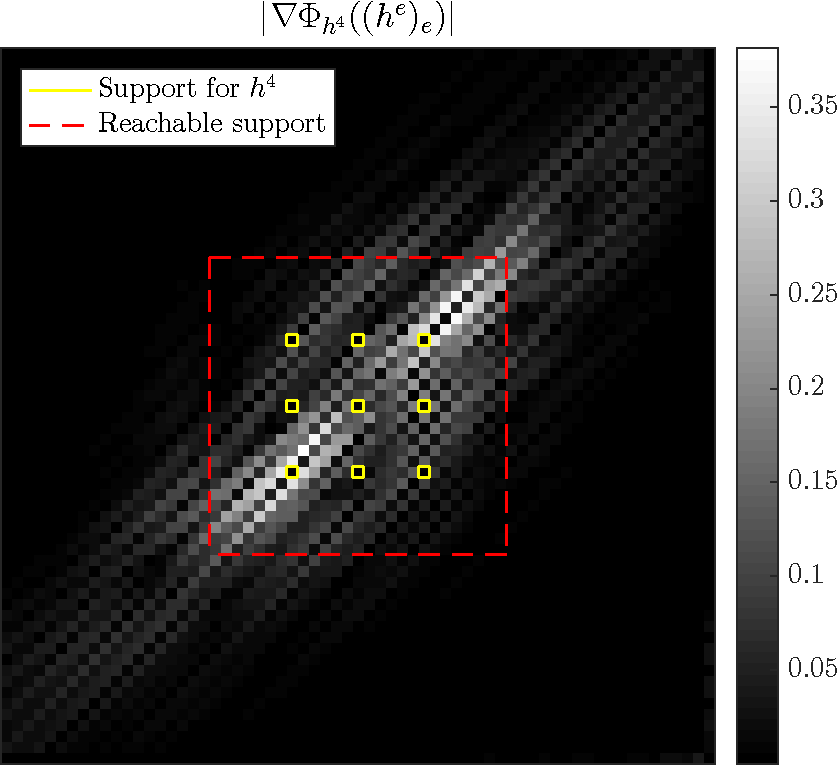
\includegraphics[width=\linewidth]{figures/xp/n4/xp_128x128_sc2_angl1_K3_S3_node4_partgrad4.pdf}
	\caption{Partial gradient w.r.t.\@ $\h^4$}\label{fig_gain_n4-grad}
	\end{subfigure}
	\begin{subfigure}[b]{0.30\linewidth}\centering
	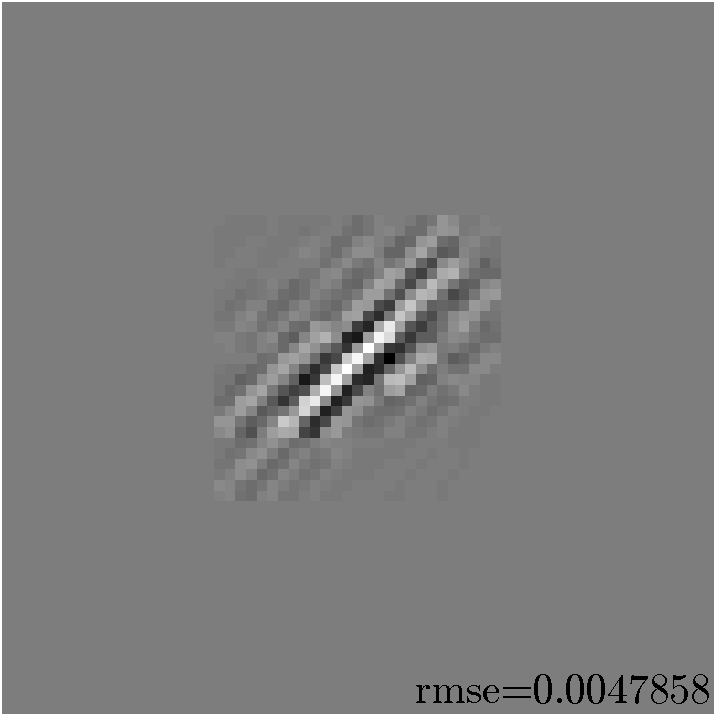
\includegraphics[width=\linewidth]{figures/xp/n4/xp_128x128_sc2_angl1_K3_S3_node4_approx.pdf}
	\caption{Approximation $\D\x$}\label{fig_gain_n4-approx}
	\end{subfigure}
	\begin{subfigure}[b]{0.34\linewidth}\centering
	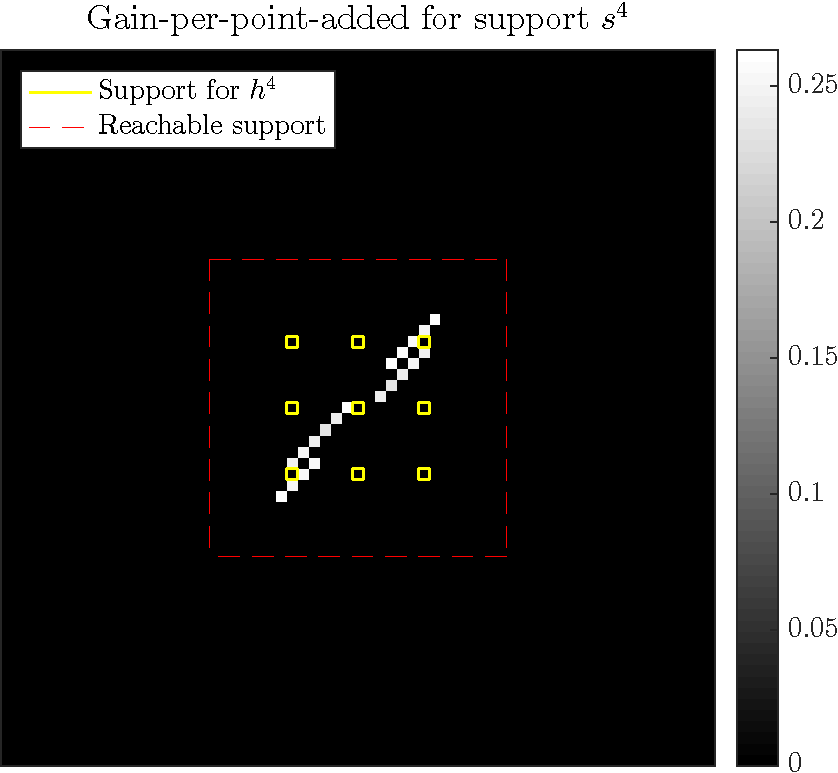
\includegraphics[width=\linewidth]{figures/xp/n4/xp_128x128_sc2_angl1_K3_S3_node4_objmatrix_bestvalues.pdf}
	\caption{Best values of above figure}\label{fig_gain_n4-gain_best}
	\end{subfigure}
	\begin{subfigure}[b]{0.34\linewidth}\centering
	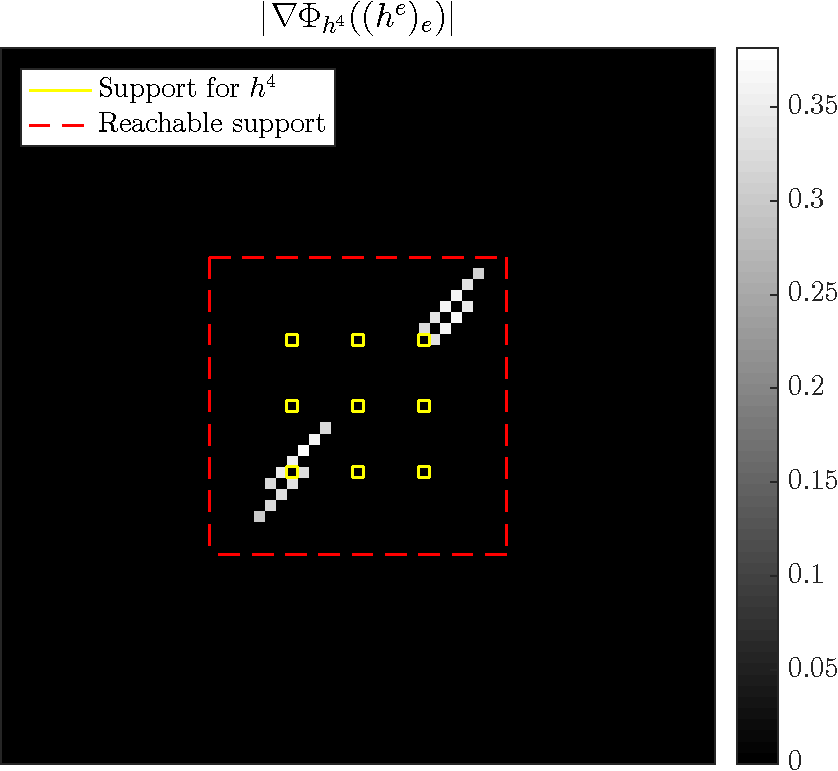
\includegraphics[width=\linewidth]{figures/xp/n4/xp_128x128_sc2_angl1_K3_S3_node4_partgrad4_bestvalues.pdf}
	\caption{Best values of above figure}\label{fig_gain_n4-grad_best}
	\end{subfigure}
\caption{Gain-per-added-point compared to “full” gradient. The “full” gradient is computed on the converged “common starting point” $\h^{\text{start}}$ (see \cref{alg_gain_per_added_point}). The gradient and gain-per-added-point maxima are almost at the same place. }\label{fig_gain_n4}
\end{figure}

\noindent
For a $128 \times 128$ target image and using the tree and codes presented in the \cref{fig_xp_explain}, the execution time of this algorithm is about 3 hours (although being parallelized on 32 threads); moreover, the algorithm must be executed each time we add an element and for each edge, thus making it practically unusable for choosing the support elements to be added.

\noindent
\Cref{fig_gain_n4} compares the gain-per-added-point of $\s^4$ (\cref{fig_gain_n4-gain}) to the absolute value of the partial gradient w.r.t.\@ $\h^4$ after a convergence of \eqref{eq_ftl} (\cref{fig_gain_n4-grad}). It is interesting to see that they share the same direction and shape. \Cref{fig_gain_n4-gain_best,fig_gain_n4-grad_best} show the best values of \cref{fig_gain_n4-gain,fig_gain_n4-grad}. We notice that the two images are reminiscent of each other and share common features: for both, we note two stripes located on the  diagonal; they only vary in that the two stripes are more distant from the center in \cref{fig_gain_n4-grad}, as if they were “dilated”. This similarity reinforces our hypothesis that the gradient could give the right information for support estimation.

\noindent
The dashed square surrounding the 9 support elements (indicated by small squares) represents the limits of the reachable support, i.e., the points that can be reached by the resulting atom (when convoluting the kernels of the branch). This explains the size restriction of the atom approximation in \cref{fig_gain_n4-appro}: outside of the reachable support, the coefficients are zeros.

\noindent
Note that the values of the gradient are equal to zero on the points of the support (small squares); with respect to those nine points, the optimality conditions are met. However, the other components of the gradient are different from zero, meaning that the solution could be improved if these components were added to the support.


\begin{figure}[!ht]\centering
	\begin{subfigure}[b]{0.24\linewidth}\centering
	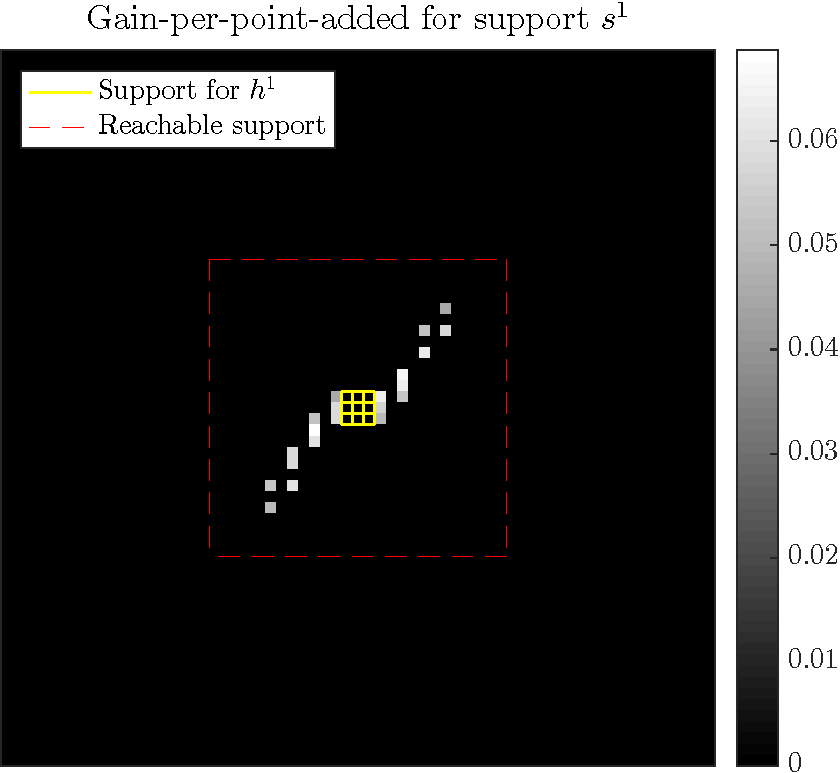
\includegraphics[width=\linewidth]{figures/xp/n1/xp_128x128_sc2_angl1_K3_S3_node1_objmatrix_bestvalues.pdf}
	\caption{$\s^1$ gain}
	\end{subfigure}
	\begin{subfigure}[b]{0.24\linewidth}\centering
	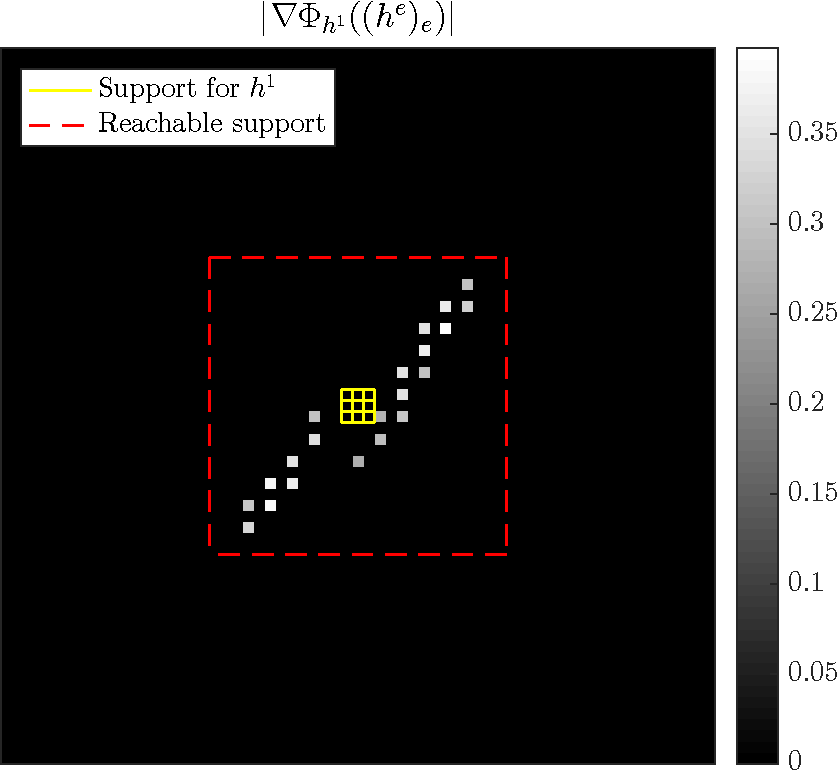
\includegraphics[width=\linewidth]{figures/xp/n1/xp_128x128_sc2_angl1_K3_S3_node1_partgrad1_bestvalues.pdf}
	\caption{$\h^1$ gradient}
	\end{subfigure}
	\begin{subfigure}[b]{0.24\linewidth}\centering
	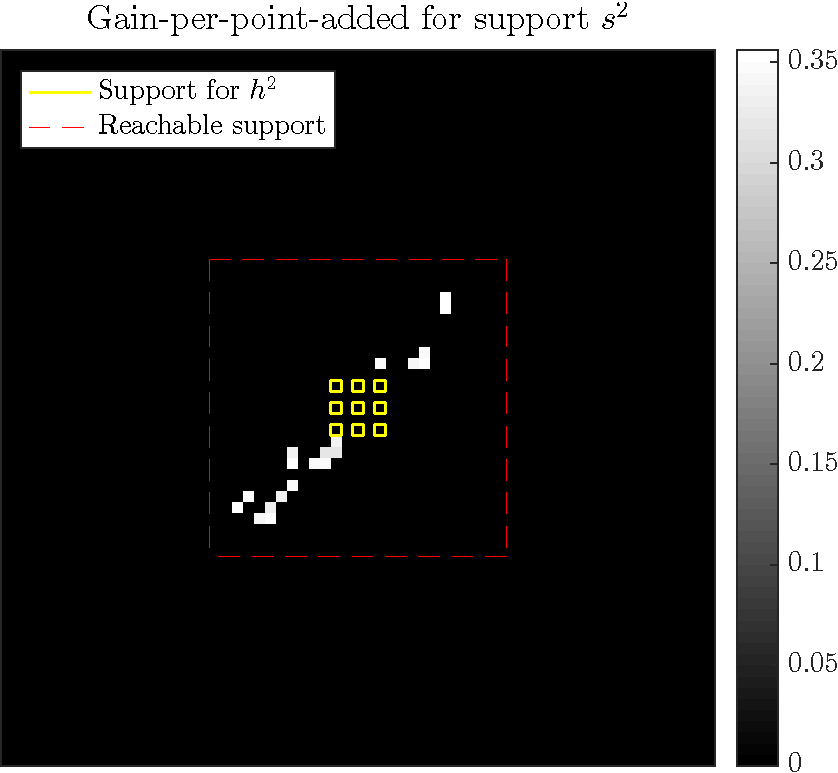
\includegraphics[width=\linewidth]{figures/xp/n2/xp_128x128_sc2_angl1_K3_S3_node2_objmatrix_bestvalues.pdf}
	\caption{$\s^2$ gain}
	\end{subfigure}
	\begin{subfigure}[b]{0.24\linewidth}\centering
	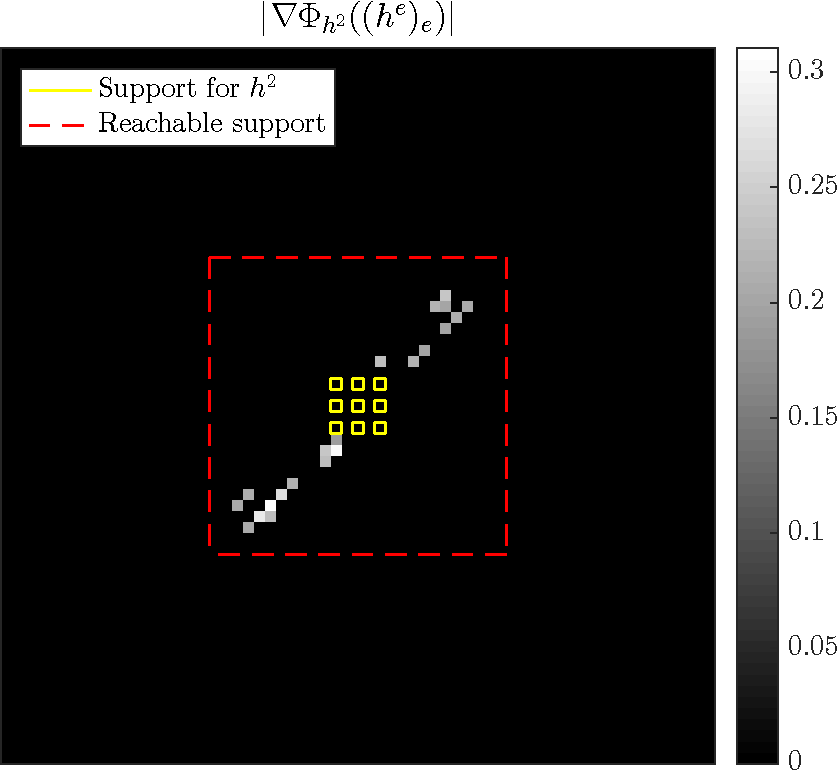
\includegraphics[width=\linewidth]{figures/xp/n2/xp_128x128_sc2_angl1_K3_S3_node2_partgrad2_bestvalues.pdf}
	\caption{$\h^2$ gradient}
	\end{subfigure}
\caption{Two other edges (1 and 2) for experiment in \cref{fig_gain_n4}. The image $\y$ and its approximation $\D\x$ are identical to \cref{fig_gain_n4}.}\label{fig_gain_n1_n2}
\end{figure}

\noindent
\Cref{fig_gain_n1_n2} does the same comparison for two other kernels of the same tree (with the same experiment). Whatever the kernel, the best values of the gradient seem to follow the same shape as the gain-per-added-point matrix. 

\begin{figure}[!ht]\centering
	\begin{subfigure}[b]{0.22\textwidth}\centering
	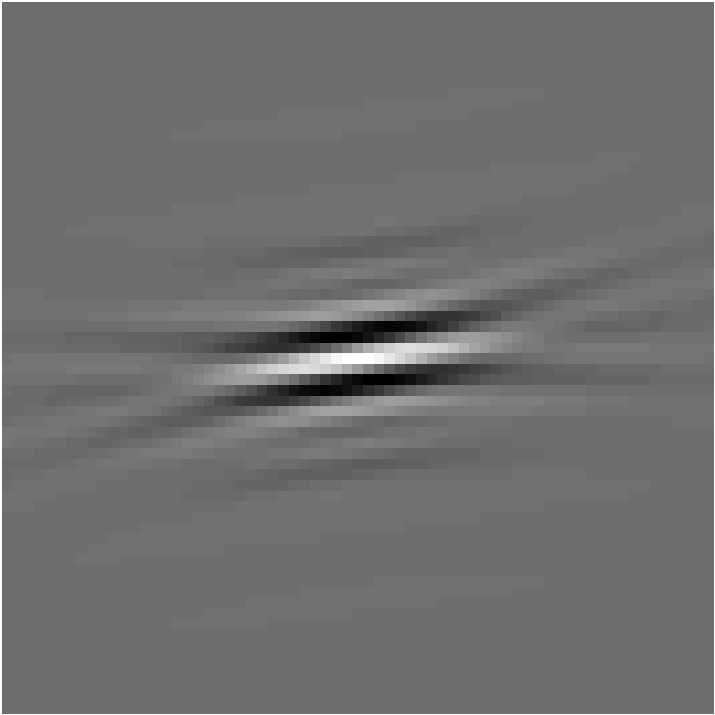
\includegraphics[width=\textwidth]{figures/xp/tilted_n4/xp_128x128_sc2_angl4_K3_S3_node4_target.pdf}
	\caption{Target $\y$}
	\end{subfigure}
	\begin{subfigure}[b]{0.22\textwidth}\centering
	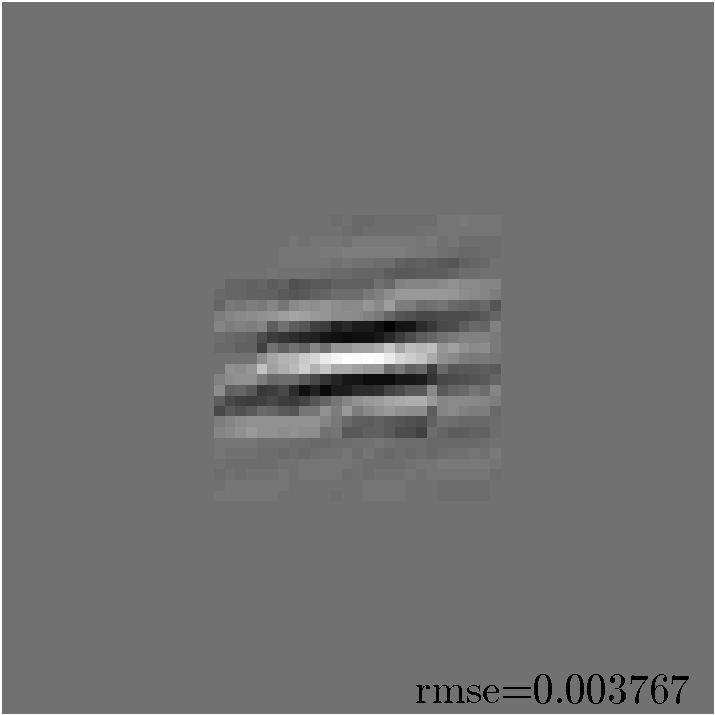
\includegraphics[width=\textwidth]{figures/xp/tilted_n4/xp_128x128_sc2_angl4_K3_S3_node4_approx.pdf}
	\caption{Approx.\@ $\D\x$}
	\end{subfigure}
	\begin{subfigure}[b]{0.26\textwidth}\centering
	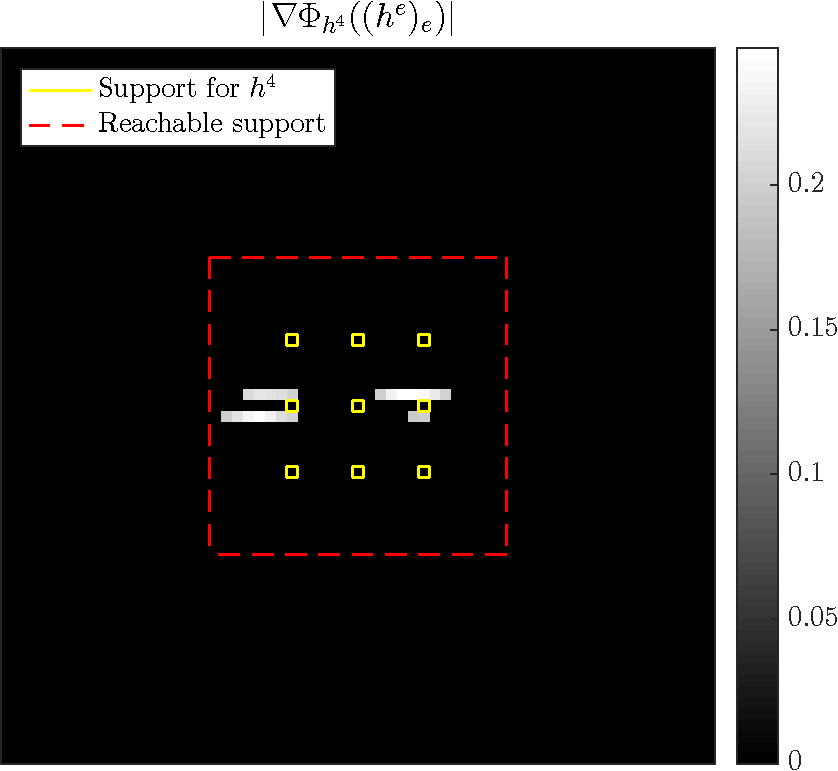
\includegraphics[width=\textwidth]{figures/xp/tilted_n4/xp_128x128_sc2_angl4_K3_S3_node4_partgrad4_bestvalues.pdf}
	\caption{$\s^4$ gain}
	\end{subfigure}
	\begin{subfigure}[b]{0.26\textwidth}\centering
	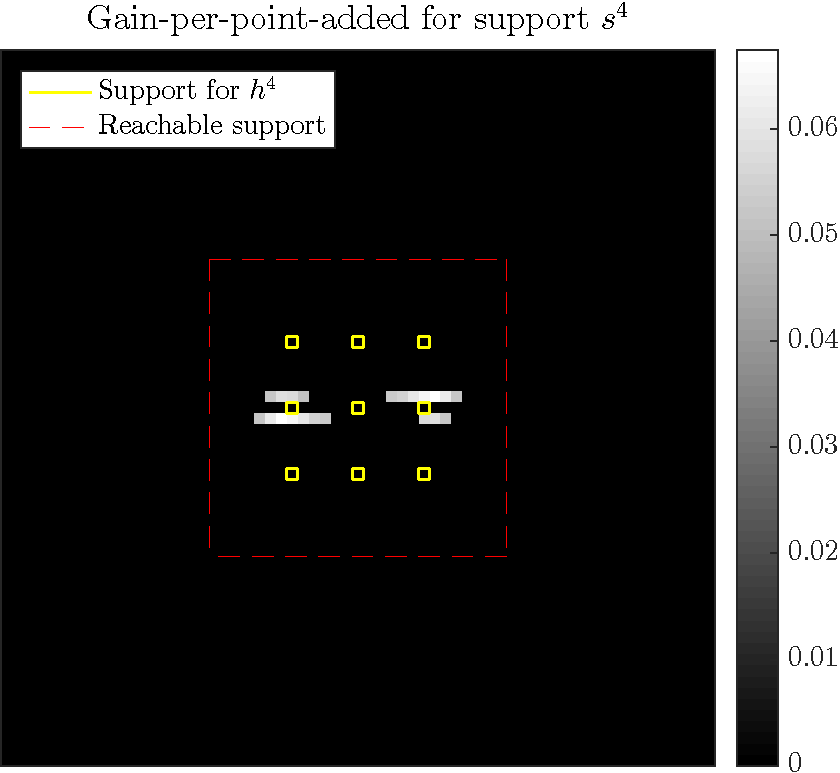
\includegraphics[width=\textwidth]{figures/xp/tilted_n4/xp_128x128_sc2_angl4_K3_S3_node4_objmatrix_bestvalues.pdf}
	\caption{$\h^4$ gradient}
	\end{subfigure}
\caption{Trying a different target image $\y$.}\label{fig_gain_tilted_n4}
\end{figure}

\noindent
Finally, \cref{fig_gain_tilted_n4} presents the same experiment but with a different target image (namely, a curvelet with a different angle). As for the two previous figures, the gradient matches the gain-per-added-point.


\FloatBarrier
\subsubsection{Visual gain when adding an element}\label{sec_visualgain}

We want to look at the improvement of the approximation when adding one support element using the gradient, compared to adding a support element using the gain-per-added-point.

\begin{figure}[!ht]\centering
\begin{subfigure}[b]{0.28\linewidth}\centering
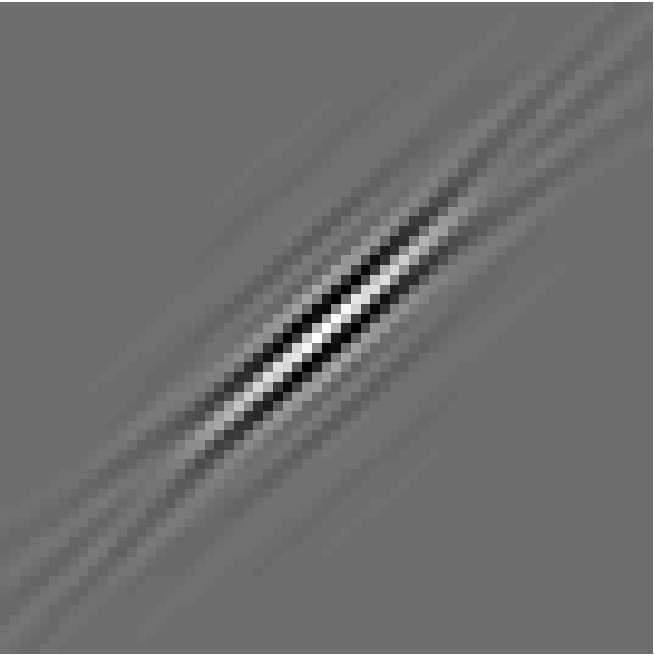
\includegraphics[width=\linewidth]{figures/before_after/target.pdf}
	\caption{Target image}\label{fig_beforeafter-target}
\end{subfigure}
\begin{subfigure}[b]{0.34\linewidth}\centering
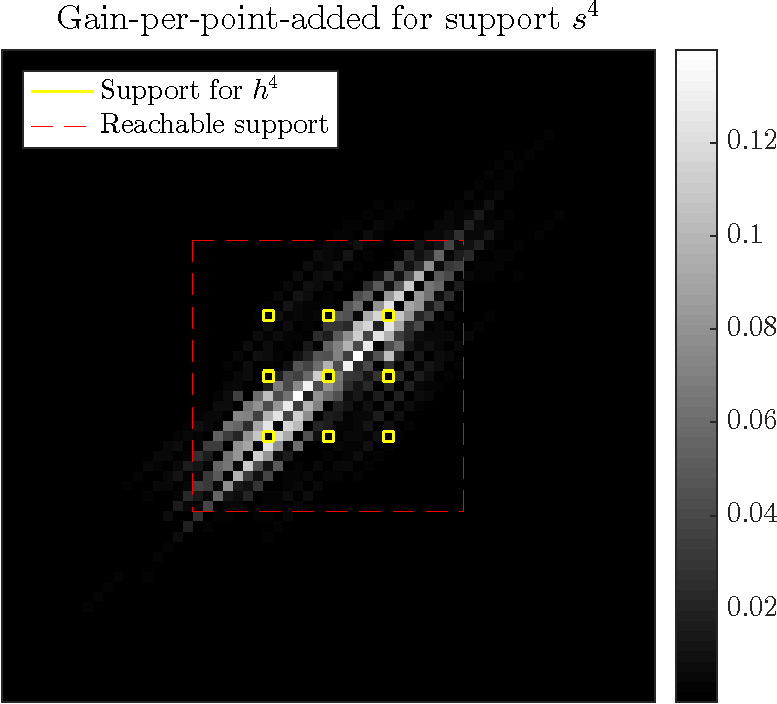
\includegraphics[width=\linewidth]{figures/before_after/before_gain.pdf}
\caption{Gain-per-added-point}\label{fig_beforeafter-gain}
\end{subfigure}
\begin{subfigure}[b]{0.34\linewidth}\centering
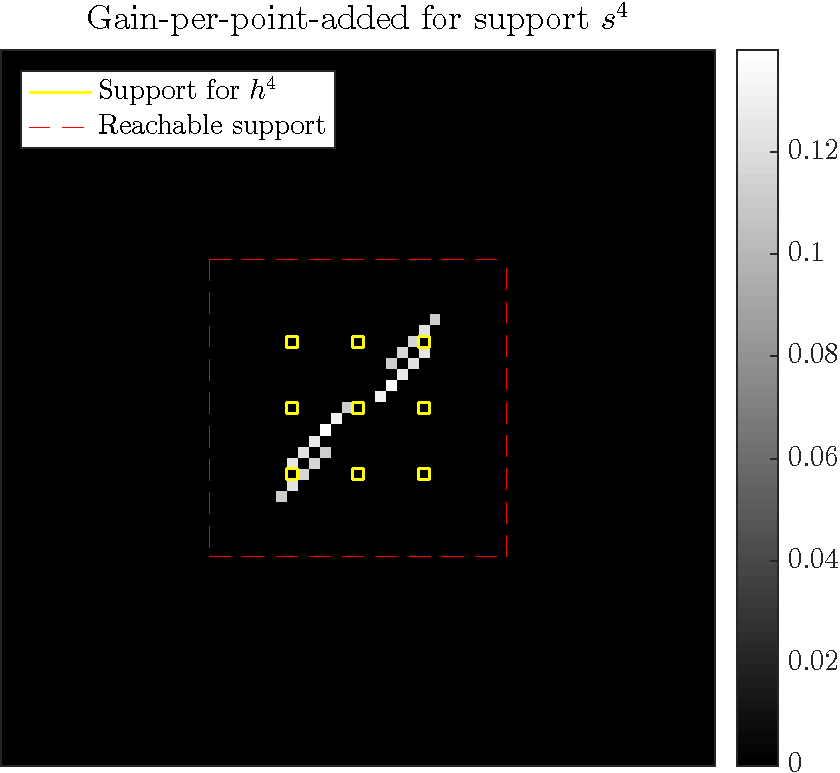
\includegraphics[width=\linewidth]{figures/before_after/before_gain_bestvalues.pdf}
\caption{Best values of \ref{fig_beforeafter-gain}}\label{fig_beforeafter-gain_best}
\end{subfigure}

\begin{subfigure}[b]{0.28\linewidth}\centering
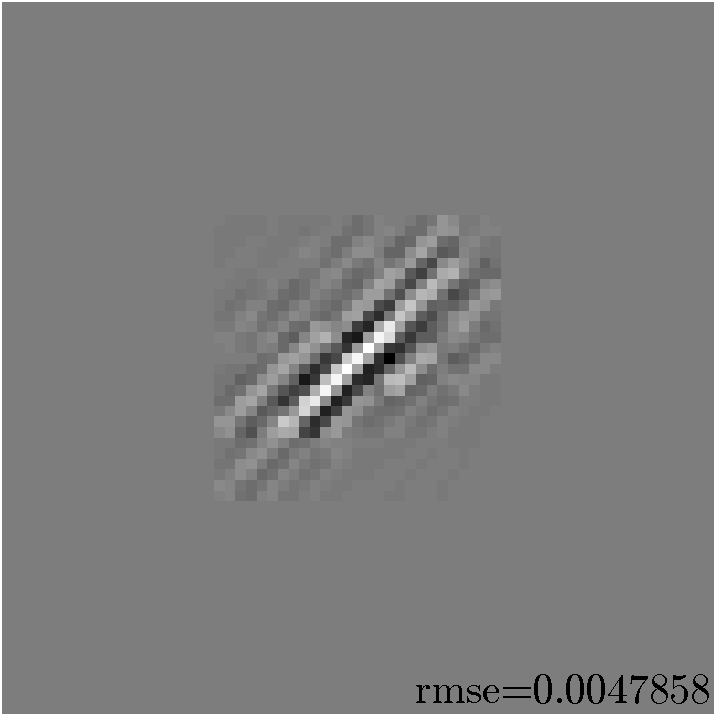
\includegraphics[width=\linewidth]{figures/before_after/before_approx.pdf}
\caption{Approx.\@ before adding}\label{fig_beforeafter-before-approx}
\end{subfigure}
\begin{subfigure}[b]{0.34\linewidth}\centering
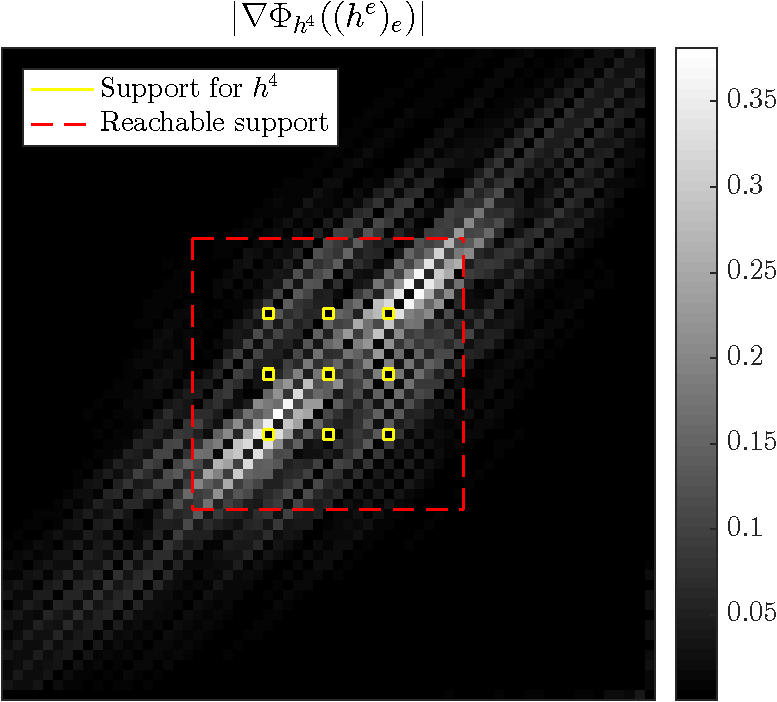
\includegraphics[width=\linewidth]{figures/before_after/before_partgrad4.pdf}
\caption{Gradient before}\label{fig_beforeafter-before-grad}
\end{subfigure}
\begin{subfigure}[b]{0.34\linewidth}\centering
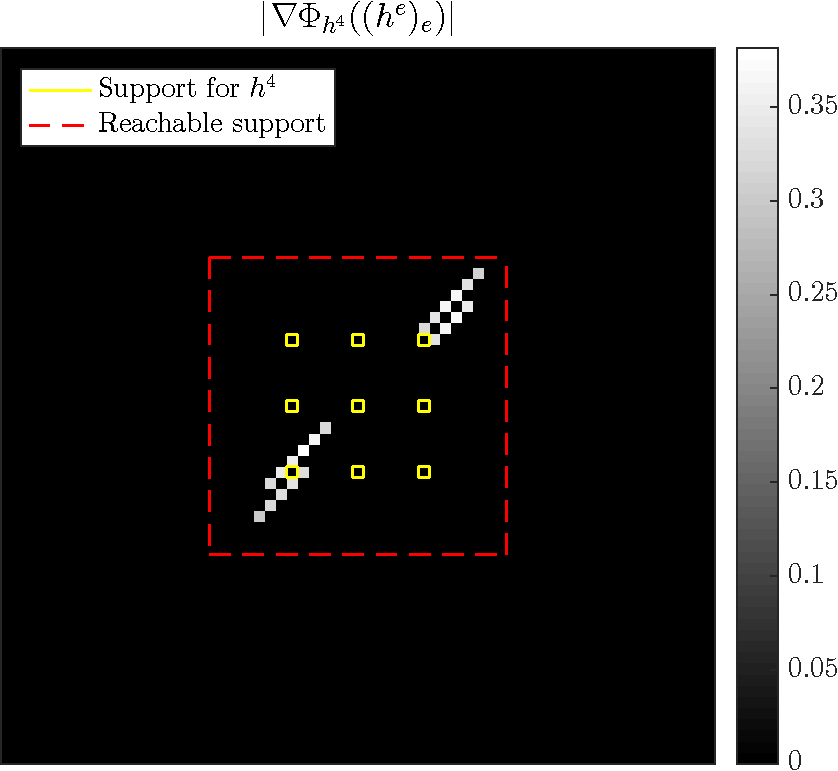
\includegraphics[width=\linewidth]{figures/before_after/before_partgrad4_bestvalues.pdf}
\caption{Best values of \ref{fig_beforeafter-before-grad}}\label{fig_beforeafter-before-grad_best}
\end{subfigure}
%\end{figure}

%\begin{figure} \ContinuedFloat
\begin{subfigure}[b]{0.28\linewidth}\centering
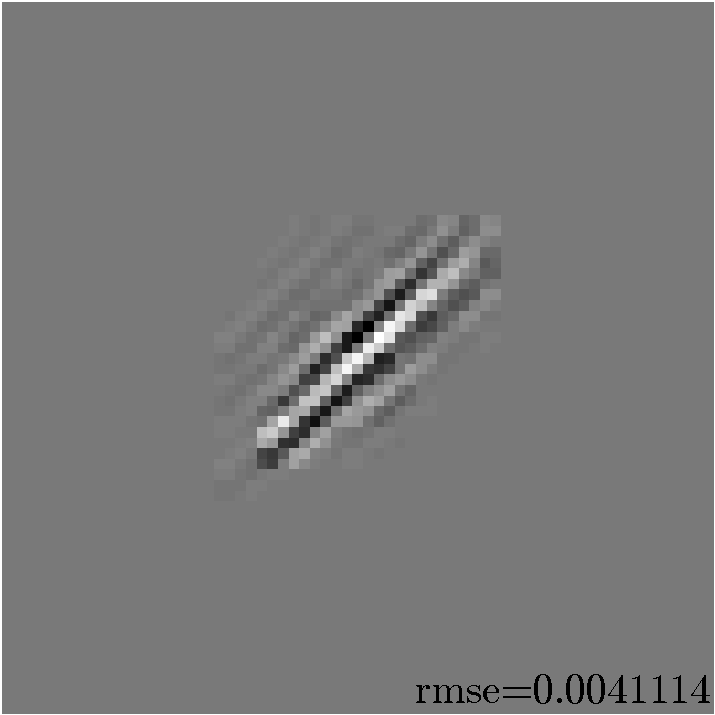
\includegraphics[width=0.94\linewidth]{figures/before_after/gainafter_approx.pdf}
\caption{Approx.\@ after adding an element using max.\@ gain}\label{fig_beforeafter-aftergainadd-approx}
\end{subfigure}
\begin{subfigure}[b]{0.34\linewidth}\centering
\includegraphics[width=\linewidth]{figures/before_after/gainafter_partgrad4.pdf}
\caption{Gradient after}\label{fig_beforeafter-aftergainadd-grad}
\end{subfigure}
\begin{subfigure}[b]{0.34\linewidth}\centering
\includegraphics[width=\linewidth]{figures/before_after/gainafter_partgrad4_bestvalues.pdf}
\caption{Best values of \ref{fig_beforeafter-aftergainadd-grad}}\label{fig_beforeafter-aftergainadd-grad_best}
\end{subfigure}
%\end{figure}

%\begin{figure} \ContinuedFloat
\begin{subfigure}[b]{0.28\linewidth}\centering
\includegraphics[width=0.94\linewidth]{figures/before_after/gradafter_approx.pdf}
\caption{Approx.\@ after adding a point using max.\@ gradient}\label{fig_beforeafter-aftergradadd-approx}
\end{subfigure}
\begin{subfigure}[b]{0.34\linewidth}\centering
\includegraphics[width=\linewidth]{figures/before_after/gradafter_partgrad4.pdf}
\caption{Gradient after}\label{fig_beforeafter-aftergradadd-grad}
\end{subfigure}
\begin{subfigure}[b]{0.34\linewidth}\centering
\includegraphics[width=\linewidth]{figures/before_after/gradafter_partgrad4_bestvalues.pdf}
\caption{Best values of \ref{fig_beforeafter-aftergradadd-grad}}\label{fig_beforeafter-aftergradadd-grad_best}
\end{subfigure}

\caption{Effect of adding one point to the support $\s^4$. The “before” tree is a converged solution of \ac{PALMTREE}. In the “after” solutions (in \cref{fig_beforeafter-aftergainadd-approx,fig_beforeafter-aftergainadd-grad,fig_beforeafter-aftergainadd-grad_best}), a point has been added where the gain-per-added-point is maximal; in \cref{fig_beforeafter-aftergradadd-approx,fig_beforeafter-aftergradadd-grad,fig_beforeafter-aftergradadd-grad_best}, a point has been added where the gradient (in absolute value) is maximal.}\label{fig_beforeafter}
\end{figure}

\noindent 
The experimental results shown in \cref{fig_beforeafter} are based on the results of \cref{fig_gain_n4-approx}, where \cref{fig_beforeafter-target,fig_beforeafter-before-approx,fig_beforeafter-gain,fig_beforeafter-before-grad,fig_beforeafter-gain_best,fig_beforeafter-before-grad_best} are the as for the previous experiment.
\Cref{fig_beforeafter-aftergainadd-approx,fig_beforeafter-aftergainadd-grad,fig_beforeafter-aftergainadd-grad_best} show what happens if we add the maximum point of gain-per-added-point to $\s^4$ and continue the minimization; in \cref{fig_beforeafter-aftergradadd-approx,fig_beforeafter-aftergradadd-grad,fig_beforeafter-aftergradadd-grad_best}, we do the same using the maximum gradient point (in absolute value). 

\noindent
We note that wether using the gain or using the gradient, the approximations (respectively in \cref{fig_beforeafter-aftergainadd-approx,fig_beforeafter-aftergradadd-approx}) look visually closer to the target image and that the RMSE is decreased respectively by 20\% and 18\%. However, the gradient indicates an element at the south-west corner of the existing support while the gain indicates a north-east element: although the best values of the gain and the gradient are located in similar places, they resulted in two different solutions.

\noindent
We also observe that after adding a point to the support (materialized by the \nth{10} small square in \cref{fig_beforeafter-aftergainadd-grad_best,fig_beforeafter-aftergradadd-grad_best}), the largest gradient values have “shifted” away from the location we added an element. Thus, adding a point to the support has an effect on the whole neighborhood.

\FloatBarrier
\subsubsection{Adding elements before the convergence of \ac{PALMTREE}}\label{sec_add_before_converged}

When looking at \cref{alg_omppalmtree_ftl} of \cref{alg_omppalmtree} where a “full” minimization is performed (i.e., it stops as soon as \ac{PALMTREE} has converged), we wondered if it was necessary to wait until convergence. Because the minimization takes a lot of time, it is tempting to try adding elements every few iterations of \ac{PALMTREE}.

\noindent
Previously, we have seen in \Cref{fig_gain_n4} that the “full” gradient can be satisfactorily used for adding elements to the support $\s$, provided that \cref{alg_palmtree} at \cref{alg_omppalmtree_ftl} has converged. Would the gradient still give a valid information on a not-yet converged solution of \ac{PALMTREE}, for example after 5 iterations instead of the $\sim{}300$ iterations for convergence?

\begin{figure}[!ht]\centering
\begin{subfigure}[b]{0.49\linewidth}\centering
\includegraphics[width=\linewidth]{figures/xp_grad_iterations/xp_128x128_sc2_angl1_K3_S3_node4_objmatrix_bestvalues.pdf}
\caption{Gain-per-added-point matrix}
\end{subfigure}
\begin{subfigure}[b]{0.49\linewidth}\centering
	\begin{subfigure}[b]{0.49\linewidth}\centering
	\includegraphics[width=\linewidth]{figures/xp_grad_iterations/xp_128x128_sc2_angl1_K3_S3_node4_iter1_partgrad4_bestvalues.pdf}
	\caption{Grad.\@ iter.\@ 1}
	\end{subfigure}
	\begin{subfigure}[b]{0.49\linewidth}\centering
	\includegraphics[width=\linewidth]{figures/xp_grad_iterations/xp_128x128_sc2_angl1_K3_S3_node4_iter8_partgrad4_bestvalues.pdf}
	\caption{Grad.\@ iter.\@ 8}
	\end{subfigure}
	\begin{subfigure}[b]{0.49\linewidth}\centering
	\includegraphics[width=\linewidth]{figures/xp_grad_iterations/xp_128x128_sc2_angl1_K3_S3_node4_iter20_partgrad4_bestvalues.pdf}
	\caption{Grad.\@ iter.\@ 20}
	\end{subfigure}
	\begin{subfigure}[b]{0.49\linewidth}\centering
	\includegraphics[width=\linewidth]{figures/xp_grad_iterations/xp_128x128_sc2_angl1_K3_S3_node4_iter200_partgrad4_bestvalues.pdf}
	\caption{Grad.\@ iter.\@ 200}
	\end{subfigure}
\end{subfigure}
\caption{Is the gradient giving the same information depending on the iteration of \ac{PALMTREE}? This is the same experiment as \cref{fig_gain_n4}. Only the best values are displayed.}\label{fig_iter_gain_vs_grad}
\end{figure}

\noindent
\Cref{fig_iter_gain_vs_grad} compares the best values of gain-per-added-point to gradient snapshots obtained during the minimization. This result is encouraging: whatever the iteration, the gradient best values stay close to the gain-per-added-point best values. We conclude that adding elements every few iterations of \ac{PALMTREE} can provide interesting results.

\FloatBarrier
\section{Learning the supports for a single branch}

In the previous section, we showed that the gradient gives a good indication on which support elements should be added. In this section, we study the use of the gradient for learning the support $\s$ on a simple single-branch, using the \cref{alg_omppalmtree}. 

\noindent
According to the conclusions of \cref{sec_add_before_converged} that indicate that the convergence of \ac{PALMTREE} is not mandatory before adding an element, we simply set a maximum number of iterations for \ac{PALMTREE}, denoted by $T$.

\begin{figure}[!ht]\centering
\begin{subfigure}[b]{0.085\textwidth}\centering
	\includegraphics[width=\textwidth]{figures/exple-better-support/tree_classic.pdf}
	\caption{}\label{fig_learnsupp_branch-generic_tree}
\end{subfigure}
\begin{subfigure}[b]{0.39\textwidth}\centering
\includegraphics[width=\textwidth]{figures/exple-better-support/xp_128x128_sc2_angl1_K3_S3_node4classic_approx.pdf}
\caption{Approx.\@ $\D\x$ with generic supports}\label{fig_learnsupp_branch-generic_approx}
\end{subfigure}
\begin{subfigure}[b]{0.085\textwidth}\centering
\includegraphics[width=\textwidth]{figures/variable_support/support.pdf}
\caption{}\label{fig_learnsupp_branch-learned_tree}
\end{subfigure}
\begin{subfigure}[b]{0.39\textwidth}\centering
\includegraphics[width=\textwidth]{figures/variable_support/xp_128x128_sc2_angl1_K3_S3_node4_variable_approx.pdf}
\caption{Approx.\@ $\D\x$ with learned supports}\label{fig_learnsupp_branch-learned_approx}
\end{subfigure}
\caption{Learning the supports for a single branch. Starting from Diracs, the best element is added to one of the supports every 5 iterations, up to 36 elements. The target image $\y$ is the same as in \cref{fig_gain_n4-target}.}\label{fig_learnsupp_branch}
\end{figure}

\noindent
In \cref{fig_learnsupp_branch-learned_tree}, the initial supports are simply centered Diracs; every $T=5$ iterations of \ac{PALMTREE}, one element is added at the location of the largest gradient, up to 36 elements. The OMP-PALMTREE algorithm (\cref{alg_omppalmtree}) converges after a cumulative number of 200 iterations of \ac{PALMTREE}.

\noindent
The resulting approximation plotted in \cref{fig_learnsupp_branch-learned_approx} is encouraging with a relative RMSE decrease of 76\% compared to the approximation in \cref{fig_learnsupp_branch-generic_approx} using the generic supports in \cref{fig_learnsupp_branch-generic_tree}.

%\begin{subfigure}[b]{1\textwidth}\centering
%\includegraphics[width=\textwidth]{figures/variable_support/xp_128x128_sc2_angl1_K3_S3_node4_variable_target.pdf}
%\caption{Image $\y$}
%\end{subfigure}

\FloatBarrier
\section{Learning supports for a tree}

The previous section has shown encouraging results for a single branch dictionary. In this section, we investigate the use of the gradient for adding support elements in a tree. More specifically, we study two sub-problems that came up with the use of the tree:
\begin{enumerate}[label=--,noitemsep,nolistsep]
	\item \emph{How to prevent the elements from being scattered?} For this problem, we propose a simple prior based on the distance to the center of the gradient;
	\item \emph{How to prevent the number of elements per support from being unbalanced?} In order to solve this issue, we present a modified prior function which takes into account the specificity of every support.
\end{enumerate}


\subsection{Experimental setup}

For testing our support learning algorithm OMP-PALMTREE (\cref{alg_omppalmtree}), we propose to use the convolutional tree defined in \cref{fig_learntree_setup}. The target $\y$ in \cref{fig_learntree_setup-target} is made of curvelets at different scales and angles; from left to right and top to bottom, the 16 curvelets of $\y$ (numbered 1 through 16) have the corresponding codes $\x^l$ with $l=1,\dots,16$. Note that the codes are located at the centers of their corresponding curvelets, as shown in \cref{fig_learntree_setup-codes}.
The following experiments using OMP-PALMTREE have been set such that
\begin{enumerate}[label=(\roman*),noitemsep,nolistsep]
\item at the PALMTREE minimization step, PALMTREE does a maximum of 5 iterations (as discussed in \cref{sec_add_before_converged});
\item at the “adding elements” step, 5 elements are added instead of only 1 in order to decrease the number of iterations necessary for adding the 279 elements. This choice can be subject to discussion: the multiple added elements may end up enhancing the same atom, possibly making some of the added elements useless because of their proximity (as discussed at the end of \cref{sec_visualgain}). We tried to limit this effect by adding the elements in separate supports.
\end{enumerate}

\begin{figure}[!ht] \centering
\begin{subfigure}[b]{0.325\textwidth}\centering
\includegraphics[width=\textwidth]{figures/tree-learn-setup/target.pdf} 
	\caption{Target image $\y$}\label{fig_learntree_setup-target}
\end{subfigure}
\begin{subfigure}[b]{0.325\textwidth}\centering
\includegraphics[width=\textwidth]{figures/tree-learn-setup/tree.pdf}
	\caption{Tree defining $\D$}\label{fig_learntree_setup-tree}
\end{subfigure}
\begin{subfigure}[b]{0.325\textwidth}\centering
\includegraphics[width=\textwidth]{figures/tree-learn-setup/codes.pdf} 
	\caption{Some codes $\x^l$ (4 among 16)}\label{fig_learntree_setup-codes}
\end{subfigure}
\caption{Setup of the experiments on learning the supports of a tree.}\label{fig_learntree_setup}
\end{figure}

\begin{figure}[!ht] \centering
\begin{subfigure}[b]{0.41\textwidth}\centering
\includegraphics[width=1\textwidth]{figures/tree-scattered-supports/xp_learnsupp256_curvelet_decomp3+tree-binary_dpth4+supp-diracs+usegrad0_every5_add5_totinit0_totadd279_a0_b1_approx.pdf}
\caption{Approximation $\D\x$}
\end{subfigure}
\begin{subfigure}[b]{0.56\textwidth}\centering
\includegraphics[width=1\textwidth]{figures/tree-scattered-supports/tree.pdf}
	\caption{Learned support tree}\label{fig_test_omppalmtree-tree}
\end{subfigure}
\caption{Results after using \cref{alg_omppalmtree}. Each support has been cropped to the minimal square that contains all elements; the number under each support gives the width of that square. The smaller the number is, the more gathered the elements are.}\label{fig_test_omppalmtree}
\end{figure}

\noindent 
The experiments have been run using MATLAB R2016a on a 64 cores Intel Xeon CPU E5-4650 at 2.70GHz with 512 GB of RAM. Although this server had plenty of cores, PALMTREE has not been parallelized yet, forcing us to run it on a single processor. However, the many available cores have been useful for launching many runs of the algorithm (e.g., for trying many parameters).

\noindent
A first result using the original OMP-PALMTREE (\cref{alg_omppalmtree}) is displayed in \Cref{fig_test_omppalmtree}. Note that we cannot distinguish the elements of the supports. A zoom on one of the supports is made in \cref{fig_scattered_support-tree} (section below).

\subsection{Problem of scattered elements using \cref{alg_omppalmtree}}
 
An unexpected issue was observed in \cref{fig_test_omppalmtree} when running the \cref{alg_omppalmtree} on a tree instead of a single branch: as shown in \cref{fig_scattered_support-tree}, the elements of the learned supports are scattered in distant clusters. 

\begin{figure}[!ht] \centering
\begin{subfigure}[b]{0.65\textwidth}\centering
\includegraphics[width=1\textwidth]{figures/tree-scattered-supports/supports_with_zoom.pdf}
\caption{Supports with magnified $\s^1$}\label{fig_scattered_support-tree}
\end{subfigure}
\begin{subfigure}[b]{0.34\textwidth}\centering
\includegraphics[width=1\textwidth]{figures/tree-scattered-supports/_partgrad1.pdf}
\caption{Gradient for $\h^1$}\label{fig_scattered_support-grad}
\end{subfigure}
\caption{Scattered supports when using the original OMP-PALMTREE (\cref{alg_omppalmtree}). The gradient in (b) has its maximum values in distant locations, therefore producing scattered supports.}\label{fig_scattered_support}
\end{figure}

\noindent
This can be interpreted as an identifiability problem of the atoms (one feature corresponds to one curvelet among the 16 that form the target).
An atom is said to be well identified when it can explain one feature of the image without any contributions from the other atoms. A poorly identified atom will result in having features that are represented using multiple atoms at once. For example, in our experiments, the 16 curvelets of the target image are 16 different features. The learned dictionary can be either composed of 16 well identified atoms (one atom represents one feature) or it can be composed of a “single” huge atom that is made of 16 small and scattered pieces.
The latter can be interpreted as an instance of overfitting, that is, the learned atoms are too specialized with respect to the learning images and thus, cannot be used for other images.

\noindent
Ideally, we would like all elements to be centered around the origin\footnote{In the figures, the origin is at the center of the image} in order to have well identified atoms. However, the gradient in \cref{fig_scattered_support-grad} indicates elements that are far from each other, leading to scattered support elements.

\begin{algorithm}[!ht]
    \caption{OMP-PALMTREE (version 2, based on the original OMP-PALMTREE in \cref{alg_omppalmtree})}\label{alg_omppalmtree2}
  \begin{algorithmic}[1]
    \Input signal $\y$ of dimension $N$, dictionary of 
   dimension $N \times K$ with $K = |\L| \cdot N$ and $K \gg N$
    \Output A sparse code $\x$ of dimension $K$
    \State \textbf{Initialization} Initialize the supports $\s^e$ with Diracs
    \For{$i = 1,\dots,k$}
      \State $(e,p) = \underset{(e,p) \in \E \times \P}{\argmax}~ \left[ |\nabla \Phi_{\h^e}(\h)_p| \underbrace{ - \alpha~f(p)}_{\text{Concentrate the support}} \right]$\label{alg_omppalmtree2_find}
      \State $\s^e_p = 1$
      \State $\h = \underset{\h^e \in \Dspace^e}{\argmin}~ \Phi(\h)$\label{alg_omppalmtree2_ftl}
    \EndFor
  \end{algorithmic}
\end{algorithm}

\begin{figure}[!ht] \centering
\begin{subfigure}[b]{0.325\textwidth}\centering
\includegraphics[width=1\textwidth]{figures/tree-scattered-supports/grad_node1.pdf}
\caption{Gradient }\label{}
\end{subfigure}
\begin{subfigure}[b]{0.325\textwidth}\centering
\includegraphics[width=1\textwidth]{figures/tree-scattered-supports/dist_to_orig.pdf}
\caption{Function $f(p)$}\label{}
\end{subfigure}
\begin{subfigure}[b]{0.325\textwidth}\centering
\includegraphics[width=1\textwidth]{figures/tree-scattered-supports/regularized.pdf}
\caption{gradient - $f(p)$}\label{}
\end{subfigure}
\caption{Example of linear prior function using distance to origin (center of the image).}\label{fig_grad_minus_dist}
\end{figure}

\noindent
To address this issue, we add in \cref{alg_omppalmtree2} a prior term $f(p)$ (with values in $\R$) that prevents the location $p$ from being too far from the origin (center\footnotemark[1] of the support); $f$ is defined as
\begin{equation}
f(p) = \frac{\text{dist}(o-p)}{\underset{p' \in \P}{\max}~\text{dist}(o-p')} \quad \in [0,1]\label{eq_regularize}
\end{equation}
with $o$ the origin, which is the center of the support, and $\text{dist}(p)$ is the circular euclidian norm defined on $p=1,\dots,N$ by\footnotemark[2]
\begin{equation*} \text{dist}(p) = \min\left[p \bmod N, (N-p) \bmod N\right]\end{equation*}
with $\bmod$ the modulo operator. Note that $f$ simply normalizes $\text{dist}()$ in $[0,1]$. 

\noindent
\Cref{fig_grad_minus_dist} illustrates the effect of the prior $f(p)$ on the objective function (at \cref{alg_omppalmtree2_find} of \cref{alg_omppalmtree2}).



\footnotetext[1]{Note that the actual implementation relies on kernels centered on the origin $(1,1)$; for easier understanding, we translate the kernels so that the origin is centered.}
\footnotetext[2]{Note that the actual implementation uses non-vectorized images (matrices). This implies that this definition must be extended to two dimensional $\bm{p} = \begin{bmatrix}
	p_1 \\ p_2\end{bmatrix}$. It is easily done with 
	$\text{dist}(\bm{p}) = \left\| \begin{bmatrix} \text{dist}(p_1) \\ \text{dist}(p_2)\end{bmatrix} \right\|_2$.}



\subsection{Tuning the prior parameter $\alpha$}
In the previous section, we proposed the prior $f$, which means that we must deal with an additional parameter $\alpha$.

\subsubsection{Ad hoc tuning of $\alpha$}\label{sec_tuning_alpha}
\begin{figure}[!ht] \centering
\includegraphics[width=0.9\textwidth]{figures/tree-scattered-supports/gradient_used.pdf}
	\caption{Blind tuning of $\alpha$} \label{fig_tuning_alpha}
\end{figure}

A straightforward way of finding the right $\alpha$ is to try every possible value. We launched the algorithm for every $\alpha$ ranging from 0 to 70. \Cref{fig_tuning_alpha} compares the RMSE and computation time of OMP-PALMTREE with respect to $\alpha$. The optimal $\alpha$ seems to be around 10. 

\noindent
Note that the mentioned “slow convolutions” can be simply interpreted as an consequence of the implementation: the more elements the central kernel $\h^1$ (and its children) have, the slower the overall convolutions are.

\noindent
This brute-force method could be a possible way of tuning the $\alpha$. However, it requires many runs of OMP-PALMTREE. The average time of one run being about 200 seconds, using the algorithm is not conceivable.

\begin{figure}[!ht] \centering
\begin{subfigure}[b]{0.49\textwidth}\centering
\includegraphics[width=0.8\textwidth]{figures/tree-unbalanced-supp/xp_learnsupp256_curvelet_decomp3[tree-binary_dpth4]_supp-diracs_[usegrad1_every5_add5_totinit0_totadd279_alpha10]_approx.pdf}
\caption{Approx.\@ $\D\x$ using prior $f$ ($\alpha=10$)}\label{fig_test_omppalmtree2-approx_alpha10}
\end{subfigure}
\begin{subfigure}[b]{0.49\textwidth}\centering
\includegraphics[width=0.8\textwidth]{figures/tree-unbalanced-supp/xp_learnsupp256_curvelet_decomp3[tree-binary_dpth4]_supp-diracs_[usegrad1_every5_add5_totinit0_totadd279_alpha10]_tree.pdf}
\caption{Support tree using prior $f$ ($\alpha=10$)}\label{fig_test_omppalmtree2-tree_alpha10}
\end{subfigure}
%\end{figure}
%\begin{figure}[!ht] \ContinuedFloat
\begin{subfigure}[b]{0.49\textwidth}\centering
\includegraphics[width=0.8\textwidth]{figures/tree-unbalanced-supp/xp_learnsupp256_curvelet_decomp3[tree-binary_dpth4]_supp-diracs_[usegrad1_every5_add5_totinit0_totadd279_alpha30]_approx.pdf}
\caption{Approx.\@ $\D\x$ using prior $f$ ($\alpha=30$)}\label{fig_test_omppalmtree2-approx_alpha30}
\end{subfigure}
\begin{subfigure}[b]{0.49\textwidth}\centering
\includegraphics[width=0.8\textwidth]{figures/tree-unbalanced-supp/xp_learnsupp256_curvelet_decomp3[tree-binary_dpth4]_supp-diracs_[usegrad1_every5_add5_totinit0_totadd279_alpha30]_tree.pdf}
\caption{Support tree using prior $f$ ($\alpha=30$)}\label{fig_test_omppalmtree2-tree_alpha30}
\end{subfigure}
\caption{Learned dictionary using \cref{alg_omppalmtree2} with $\alpha=10$ and $\alpha=30$. The target image $\y$ is the same as in \cref{fig_learntree_setup-target}.}\label{fig_test_omppalmtree2}
\end{figure}

\noindent
\Cref{fig_test_omppalmtree2} gives the result for $\alpha=10$ and $\alpha=30$. Compared to \cref{fig_test_omppalmtree}, the prior with $\alpha=10$ improves the RMSE by 47\% (29\% for $\alpha=30$). It confirms our intuition that preventing “scattered” supports lead to better approximations.


%\begin{algorithm}[!ht]
%    \caption{Bruteforce method for estimating $\alpha$}\label{alg_alpha_bruteforce_method}
%  \begin{algorithmic}[0]
%  	\State Set $\alpha$ to a large value, set $r < 1$
%  	\Repeat
%	  	\State Run OMP-PALMTREE using $\alpha$
%	  	\State $\alpha \leftarrow r\alpha$
%  	\Until{stopping criteria is met}
%\end{algorithmic}
%\end{algorithm}

\FloatBarrier
\subsubsection{Estimating $\alpha$ from the data}

The prior parameter $\alpha$ should be estimated from the target image, meaning that finding the right $\alpha$ should be a part of the algorithm. Many methods are available in the literature; one of the simplest is the Blind Method proposed in \cite{almeida_parameter_2013}. We can also mention the state-of-the-art SURE method (Stein’s unbiased risk estimate), proposed in \cite{eldar_generalized_2009} as well as the Bayesian regularization method developed in \cite{archer_bayesian/regularization_1995}.

\noindent
These algorithms have not been investigated during this internship and will be conducted in a PhD thesis.

\subsection{Problem with the prior: unbalanced supports}\label{sec_pbm_unbalanced_supports}
The prior allowed us to prevent scattered supports; another problem probably caused by the gradient is the “unbalanced” supports: some supports contain most elements, while others have only one or two elements. 

\begin{figure}[!ht] \centering
\begin{subfigure}[b]{1\textwidth}\centering
\includegraphics[width=0.6\textwidth]{figures/tree-unbalanced-supp/tree-unbalanced.pdf}
\end{subfigure}
\caption{Problem of unbalanced support choosing ($\alpha=10$).}\label{fig_unbalanced_supports}
\end{figure}

% The reason why we need “balanced” supports is linked to another research axis we would like to explore: learning the tree. In fact, if a support becomes a single Dirac, we can remove the edge it is associated with. This means that learning the tree 

\noindent
The reason why we need “balanced” supports is that an overly-complex support (like the middle one in \cref{fig_unbalanced_supports}) makes the convolution slow. The more uniformly distributed the support elements are, the faster the convolution.

% In the couple $(e,p)$ chosen by the gradient, the choice of the support edge $e$ does not seem to effective, although the choice of $p$ is valid (as discussed in \cref{sec_gain_per_added_point}).

\noindent
\Cref{fig_unbalanced_supports} illustrates this issue: with $\alpha=10$, most elements have been added on the support $\s^1$, while $\s^{27}$ has only 3 elements.

\noindent
We found out that adjusting the prior parameter $\alpha$ is not enough if we want “balanced” supports. We could simply make $\alpha$ dependent of $e$, which could lead to the following “find support element to add” step
\begin{equation}
(e,p) = \underset{(e,p) \in \E \times \P}{\argmax}~ |\nabla \Phi_{\h^e}(\h)_p| - \alpha_e f(p)
\end{equation}
with $\bm{\alpha} = \begin{bmatrix}\alpha_1 & \dots & \alpha_{|\E|}\end{bmatrix}$. However, estimating this vector $\bm{\alpha}$ requires even more complex algorithms. We let this possibility to future studies.

\subsubsection{Empirical workaround using one single $\alpha$}
Instead of estimating the vector $\bm{\alpha}$, we empirically developed a function $f$ for balancing the number of elements per support using one single $\alpha$. This method requires $\alpha$ to be estimated, though. The prior function is
\begin{equation}
f’(\h,e,p) = \frac{\text{dist}(o-p)}{\underset{p' \in \P}{\max}~\text{dist}(o-p')} \cdot G(\h,e) \quad \in [0,G(\h,e)]\label{eq_regularize2}
\end{equation}
where $G(\h,e)=\underset{p' \in \P}{\max}~ |\nabla \Phi_{\h^e}(\h)_{p'}|$ is the maximum value of the partial gradient w.r.t. $h^e$.

\noindent
This prior function is simply adjusted with respect to the amplitude of each partial gradient. This result is totally empirical and has not been proved (it may even lead to suboptimal supports).

\begin{figure}[!ht] \centering
\begin{subfigure}[b]{0.49\textwidth}\centering
\includegraphics[width=0.8\textwidth]{figures/tree-gradient-vs-sequential/xp_learnsupp256_curvelet_decomp3_tree-binary_dpth4_supp-diracs_usegrad1_every5_add5_totinit0_totadd279_alpha30_tree.pdf}
	\caption{Supports chosen using prior $f’$ ($\alpha=30$)}\label{fig_cmpunbalanced-grad_tree}
\end{subfigure}
\begin{subfigure}[b]{0.49\textwidth}\centering
\includegraphics[width=0.8\textwidth]{figures/tree-gradient-vs-sequential/xp_learnsupp256_curvelet_decomp3_tree-binary_dpth4_supp-diracs_usegrad1_every5_add5_totinit0_totadd279_alpha30_approx.pdf}
	\caption{Approx.\@ $\D\x$ for prior $f’$ ($\alpha=30$)}\label{fig_cmpunbalanced-grad_approx}
\end{subfigure}
%\end{figure}
%\begin{figure}[!ht] \ContinuedFloat
\begin{subfigure}[b]{0.49\textwidth}\centering
\includegraphics[width=0.8\textwidth]{figures/tree-gradient-vs-sequential/xp_learnsupp256_curvelet_decomp3_tree-binary_dpth4_supp-diracs_usegrad0_every5_add5_totinit0_totadd279_alpha30_tree.pdf} 
	\caption{Supports chosen sequentially}\label{fig_cmpunbalanced-seq_tree}
\end{subfigure}
\begin{subfigure}[b]{0.49\textwidth}\centering
\includegraphics[width=0.8\textwidth]{figures/tree-gradient-vs-sequential/xp_learnsupp256_curvelet_decomp3_tree-binary_dpth4_supp-diracs_usegrad0_every5_add5_totinit0_totadd279_alpha30_approx.pdf} 
	\caption{Approx.\@ $\D\x$ for sequential variant}\label{fig_cmpunbalanced-seq_approx}
\end{subfigure}
\caption{Comparison of sequential versus using the gradient when choosing a support for adding an element. The target image $\y$ is the same as in \cref{fig_learntree_setup-target}.}\label{fig_cmpunbalanced-seq_vs_grad}
\end{figure}

\FloatBarrier
\noindent
We compared in \cref{fig_cmpunbalanced-seq_vs_grad} the results using $f’$ against a modified version of OMP-PALMTREE where the elements are added sequentially on every support.
\begin{enumerate}[label=(\roman*),noitemsep,nolistsep]
	\item In \cref{fig_cmpunbalanced-grad_tree}, $e$ and $p$ are both chosen using the gradient;
	\item In \cref{fig_cmpunbalanced-seq_tree}, $p$ is chosen using the gradient, $e$ is sequentially selected: we add an element to $\s^1$, then to $\s^2$\dots so that every support has the exact same number of elements.
\end{enumerate}


\begin{figure}[!ht] \centering
\begin{subfigure}[b]{0.325\textwidth}\centering
\includegraphics[width=\textwidth]{figures/tree-unbalanced-supp/histo_alpha10_grad1.pdf}
	\caption{Distribution of \cref{fig_test_omppalmtree2-approx_alpha10} (using prior $f$)}\label{fig_histo-1}
\end{subfigure}	
\begin{subfigure}[b]{0.325\textwidth}\centering
\includegraphics[width=\textwidth]{figures/tree-gradient-vs-sequential/histo_alpha30_grad1.pdf}
	\caption{Distribution of \cref{fig_cmpunbalanced-grad_tree} (using prior $f’$)}\label{fig_histo-2}
\end{subfigure}
\begin{subfigure}[b]{0.325\textwidth}\centering
\includegraphics[width=\textwidth]{figures/tree-gradient-vs-sequential/histo_alpha30_grad0.pdf} 
	\caption{Distribution of \cref{fig_cmpunbalanced-seq_tree} (sequential variant)}\label{fig_histo-3}
\end{subfigure}	
\caption{Comparison of the distributions of the elements in supports.}\label{fig_histo}
\end{figure}

\noindent
Sequentially choosing the support for adding a new element in \cref{fig_cmpunbalanced-grad_tree} obviously leads to uniformly distributed supports (distribution shown in \cref{fig_histo-3}). \Cref{fig_histo-1,fig_histo-2} compare the distributions of elements of the trees in (respectively) \cref{fig_test_omppalmtree2-approx_alpha10,fig_cmpunbalanced-grad_tree}. And as we wanted, using $f’$ instead of $f$ gives more balanced supports, with a drop in standard deviation of $62\%$. Curiously, choosing the supports sequentially gives better results in terms of RMSE.


\begin{figure}[!ht] \centering
\begin{subfigure}[b]{0.49\textwidth}\centering
\includegraphics[width=\textwidth]{figures/tree-gradient-vs-sequential/gradient_used.pdf}
	\caption{Using $f’$ prior}\label{fig_cmp_rmse_vs_time_grad}
\end{subfigure}
\begin{subfigure}[b]{0.49\textwidth}\centering
\includegraphics[width=\textwidth]{figures/tree-gradient-vs-sequential/gradient_not_used.pdf} 
	\caption{Using the sequential variant}\label{fig_cmp_rmse_vs_time_seq}
\end{subfigure}	
\caption{RMSE versus computation time of OMP-PALMTREE for many $\alpha$}\label{fig_cmp_rmse_vs_time}
\end{figure}
\FloatBarrier

\noindent
\Cref{fig_cmp_rmse_vs_time} compares the RMSE to the time spent running OMP-PALMTREE for many $\alpha$ from 0 to 70. For both experiments, the best value of $\alpha$ (in term of RMSE) is located between 20 and 30. It is interesting to note that choosing the supports sequentially significantly reduces the RMSE. This results is completely unexpected and we do not have any explanation. The drop of computation time using the sequential variant has the same interpretation as discussed in \cref{fig_tuning_alpha} above.

\newcommand{\scale}{0.7}
\begin{figure}[!ht] \centering
\begin{subfigure}[b]{0.49\textwidth}\centering
\includegraphics[width=\scale\textwidth]{figures/tree-learn-setup/xp_learnsupp256_curvelet_decomp3[tree-binary_dpth4]_supp-generic3x3_[fixed-supports]_tree.pdf}
	\caption{Support tree with (fixed) generic supports}
\end{subfigure}
\begin{subfigure}[b]{0.49\textwidth}\centering
\includegraphics[width=\scale\textwidth]{figures/tree-learn-setup/xp_learnsupp256_curvelet_decomp3[tree-binary_dpth4]_supp-generic3x3_[fixed-supports]_approx.pdf}
	\caption{Approximation $\D\x$ (generic supports)}
\end{subfigure}
\begin{subfigure}[b]{0.49\textwidth}\centering
\includegraphics[width=\scale\textwidth]{figures/tree-unbalanced-supp/xp_learnsupp256_curvelet_decomp3[tree-binary_dpth4]_supp-diracs_[usegrad1_every5_add5_totinit0_totadd279_alpha10]_tree.pdf}
\caption{Support tree using prior $f$ ($\alpha=10$)}
\end{subfigure}
\begin{subfigure}[b]{0.49\textwidth}\centering
\includegraphics[width=\scale\textwidth]{figures/tree-unbalanced-supp/xp_learnsupp256_curvelet_decomp3[tree-binary_dpth4]_supp-diracs_[usegrad1_every5_add5_totinit0_totadd279_alpha10]_approx.pdf}
\caption{Approx.\@ $\D\x$ using prior $f$ ($\alpha=10$)}
\end{subfigure}
\begin{subfigure}[b]{0.49\textwidth}\centering
\includegraphics[width=\scale\textwidth]{figures/tree-gradient-vs-sequential/xp_learnsupp256_curvelet_decomp3_tree-binary_dpth4_supp-diracs_usegrad1_every5_add5_totinit0_totadd279_alpha30_tree.pdf} 
	\caption{Support tree using prior $f’$ ($\alpha=30$)}
\end{subfigure}
\begin{subfigure}[b]{0.49\textwidth}\centering
\includegraphics[width=\scale\textwidth]{figures/tree-gradient-vs-sequential/xp_learnsupp256_curvelet_decomp3_tree-binary_dpth4_supp-diracs_usegrad1_every5_add5_totinit0_totadd279_alpha30_approx.pdf} 
	\caption{Approx.\@ $\D\x$ using prior $f’$ ($\alpha=30$)}
\end{subfigure}
%\end{figure}
%\begin{figure} \ContinuedFloat
\begin{subfigure}[b]{0.49\textwidth}\centering
\includegraphics[width=\scale\textwidth]{figures/tree-gradient-vs-sequential/xp_learnsupp256_curvelet_decomp3_tree-binary_dpth4_supp-diracs_usegrad0_every5_add5_totinit0_totadd279_alpha30_tree.pdf} 
	\caption{Supports chosen sequentially}
\end{subfigure}
\begin{subfigure}[b]{0.49\textwidth}\centering
\includegraphics[width=\scale\textwidth]{figures/tree-gradient-vs-sequential/xp_learnsupp256_curvelet_decomp3_tree-binary_dpth4_supp-diracs_usegrad0_every5_add5_totinit0_totadd279_alpha30_approx.pdf} 
	\caption{Approx.\@ $\D\x$ for sequential variant}
\end{subfigure}

\caption{Comparison of the different methods used for selecting the supports.}\label{fig_learnsupp_sumup}
\end{figure}

Finally, \cref{fig_learnsupp_sumup} sums up the different approximations obtained with generic supports, using priors $f$ and $f’$ and with the sequential variant. Compared to fixed supports, using $f$, $f’$ and the sequential variant decrease the RMSE (respectively) by 59.3\%, 58.1\% and 59.6\%; the execution times are equivalent (about 80 seconds with no retries and the same stopping criteria). Although giving a larger RMSE, the prior $f’$ lead to more “balanced” distribution of the elements (and thus a lower computation time).

\FloatBarrier
\section{Conclusions and perspectives}

% Rewrite the following paragraphs in spirit of “Future work and perspectives”, instead of as a list of things that should have been done but have not.
% In general, structure 3.6 as:
% 	I. this and this and this has been done. the result is an algo that…
% 	II. that and that and that are questions to be studied in the future

% You may want to be a bit more informative on the context here and say that you consider a previously existing algo (PALMTREE) for dictionary learning, with the specificity of relying on convolutive trees for constructing atoms, yet with a priori fixed kernel supports. Here, studied: also learning the supports of the kernels from the data.


In this study, we consider a previously existing algorithm (PALMTREE) for dictionary learning, with the specificity of relying on convolutional trees for constructing atoms. Yet, this algorithm uses a priori fixed kernel supports; in this work, we studied the possibility of learning the kernel supports from the data. In order to learn the kernel supports, we investigated the use of the gradient for adding support elements in an \ac{OMP} manner. We experimentally showed that we could add multiple elements at each \ac{OMP} iteration, and that it is not necessary to do all the iterations of PALMTREE (until convergence) before going to the next OMP iteration. We proposed an  additive prior function to avoid “scattered” support elements, and modified it to favor balanced support sizes across the tree. We finally compared this prior to adding the elements sequentially on every supports.

\noindent
The result is a dictionary update algorithm (OMP-PALMTREE) that alternates between adding support elements and minimizing with PALMTREE, learning the dictionary from a single target image made of simple and well-separated curvelets and fixed codes. This algorithm yields  promising solutions compared to the “fixed supports” used in PALMTREE, with a RMSE drop of 58\% in the last experiment.

In future developments, one might want to test the algorithm on other kinds of atoms (e.g., wavelet packets, cosines; in \cite{chabiron_optimization_2016}, wavelet packets have been tested). The prior could also be subject to improvements, with for example a multiplicative prior function or the estimation of the hyper-parameter using the observed data during the algorithm. We might also be able to remove support elements, and to learn the tree (add and remove edges) along with the supports (in \cite{chabiron_optimization_2016}, a frequency-tiling-like tree design has been showed to perform much better, specifically for curvelets).

\noindent
In a broader perpective, “real” applications (such as denoising or image recognition) would require this algorithm to be used in conjunction with a sparse coding algorithm (some tests on dictionary learning have been reported in \cite{chabiron_optimization_2016}). Another important necessary development for “real” applications would be to modify the algorithm to use multiple images when learning, as well as make it scalable (like the Online Dictionary Learning algorithm).


\clearpage
\appendix

\addcontentsline{toc}{chapter}{Appendix}
\tocless\chapter{Appendix}

\section{Detail of the \ac{KSVD} algorithm}\label{sec_ksvd_detail}
\begin{algorithm}
    \caption{\ac{KSVD} (K-Singular Value Decomposition) algorithm for \eqref{eq_dl_ksvd}}\label{alg_ksvd}
  \begin{algorithmic}[1]
    \Input signal samples $\y_i$ of dimension $N$ forming the $S$ columns of $\Y$
    \Output dictionary $\D$ of dim. $K \times N$ with $K \gg N$
    \State \textbf{Initialization} Initialize $\D$ such that every column is $l^2$ normalized
    \While{not converged}
	\State For each image $\y_i$, solve \Comment{\textbf{Sparse Coding step}}\label{alg_ksvd_sparse_coding}
		\begin{align*}
			\quad \min_{\x_i}~ & \lVert \y_i-\D\x_i\rVert^2 \quad \text{s.t.}~ \lVert \x_i \rVert_0 \le \gamma
		\end{align*}
	\State $\D^{old} = \D$
	\State For each atom $\d_k^{old}$ of $\D^{old}$, \Comment{\textbf{Dictionary Update step}}\label{alg_ksvd_dict_update}
	\begin{enumerate}[leftmargin=15mm,label=(\alph*)]
		\item find the images $\y_i$ that use the atom $\d_k^{old}$, meaning $\x_i^k \ne 0$\label{item_atom_used}
		\item compute the error matrix associated with this atom,
		\begin{align*}
			\bm{E}_k = \Y-\sum_{i\ne k} \x_i^T\d_i^{old}
		\end{align*}
		\item keep only columns of $\bm{E}_k$ found in \cref{item_atom_used}
		\item Apply SVD decomposition $\bm{E}_k - \bm{U} \Delta V^T$. The first column of $\bm{U}$ becomes the new $\d_k$. $\x_k$ is updated using the first column of $\bm{V}$ multiplied by $\Delta(1,1)$ (the largest eigenvalue)
	\end{enumerate}
    \EndWhile
  \end{algorithmic}
\end{algorithm}



\FloatBarrier
\section{Link between \gls{treemodel} and dictionary matrix}\label{sec_matrix_vs_tree} 

It is useful to introduce the circulant matrix when trying to translate the convolutional product into a matrix-vector product. The circulant matrix of a vector $\h$ of dimension $N$ is defined as the $N \times N$ matrix $C(\h)$ such that
\begin{equation*}C(\h) = 
	\begin{bmatrix}
		h_1     & h_{N}   & h_{N-1} & \dots & h_{2} \\
		h_2     & h_{1}   & h_{N}   & \dots & h_{3} \\
		h_3     & h_{2}   & h_{1}   & \dots & h_{4} \\
		\vdots  &         &         &       & \vdots \\
		h_{N-1} & h_{N-2} & h_{N-3} & \dots & h_{N} \\
		h_N     & h_{N-1} & h_{N-2} & \dots & h_{1} \\
	\end{bmatrix}
.\end{equation*}

\begin{figure}[!ht] \centering
\includegraphics[width=\textwidth]{figures/block-circulant_matrix.pdf}
\caption{Rewriting the convolution into a metrix-vector product.}\label{fig_block_circular}
\end{figure}

\noindent
We can then rewrite the convolutions used in
\begin{equation*}\D\x = \sum_{l \in \L} \x^l * \h^{*l}\end{equation*}
using circular matrices. We denote $C^i = C(\h^i)$ the circular matrix for edge $i$. \Cref{fig_tree_as_matrix} compares the convolutional tree (a) to the product $\D\x$ ($\D$ being the dictionary $\D$ written as a matrix). For the convolutional tree given in (a), $\D$ can be summarized as
\begin{align}
\D = \begin{bmatrix}C^5 & C^6\end{bmatrix} \begin{bmatrix}C^1 & C^2 & 0 & 0 \\0 & 0 & C^3 & C^4\end{bmatrix}\label{eq_matrix_developed}
\end{align}
with $C^i$ the block-circular matrix for $\h^i$; it represents the final convolution $\h^{*l}*\x^l$ when using matrices.

\begin{figure}[!ht] \centering
\begin{subfigure}[b]{0.30\textwidth}\centering
\includegraphics[width=0.7\textwidth]{figures/pov-tree.pdf}
\caption{Convolutional tree}
\end{subfigure}
\begin{subfigure}[b]{0.69\textwidth}\centering
\includegraphics[width=\textwidth]{figures/pov-matrix.pdf}
\caption{Convolutional tree dictionary using a circular matrix}
\end{subfigure}
\caption{From $\D$ as a convolutional tree to $\D$ as a matrix}\label{fig_tree_as_matrix}
\end{figure}

\noindent
One atom $d_i$ with $i = 1,\dots,K$ ($K=N \cdot |\L|$) of the dictionary matrix $\D$ corresponds to one column of the block-circulant matrix $C(h^{*l})$; $\D$ can thus be rewritten as
\begin{align}\D = \begin{bmatrix} C(h^{*1}) & \dots & C(h^{*{|\L|}}) \end{bmatrix}.\label{eq_matrix_factorized} \end{align}

\noindent
To sum up, the matrix associated with the convolutional tree dictionary $\D$ can be understood as a factorization of sparse matrices $C^i$. Under the “developed” form \eqref{eq_matrix_developed}, the matrix $\D$ is of dimension $N \times K$.




\FloatBarrier
\section{Why is sparse coding used for denoising?}

\Cref{sparse_reduce_noise} shows a noisy signal $\y$ living in a high-dimensional subspace of dimension $N$ and defined by
\begin{equation*}\y=\hat{\y} + \bm{b}\end{equation*}
with $\bm{b}$ following a centered Gaussian distribution $\mathcal{N}(0,\sigma^2I)$ and $\hat{\y}$ the noiseless signal. We see that the distance $||\bm{b}||$ is always smaller than the projected distance.

\noindent
This is because the variance in the $N$-dimensional space can be written as
\begin{align*}
\mathbb{E}\left(\lVert \bm{b} \rVert^2 \right) =& \mathbb{E}\left(\sum^N_{i=1} b_i^2 \right) = \sum^N_{i=1} \mathbb{E}(b_i^2)  = N\sigma^2 \\
\Leftrightarrow \sqrt{\mathbb{E}\left(\lVert \bm{b} \rVert^2 \right)} =& \sigma \sqrt{N}.
\end{align*}
The expected norm of the noise is
\begin{equation*} \sqrt{\mathbb{E}\left(\lVert \bm{b} \rVert^2 \right)} = \sigma\sqrt{N} \end{equation*}
When projected onto the $k$-dimensional space, the expected norm of the noise becomes
\begin{equation*}\sqrt{\mathbb{E}\left(\lVert \bm{b} \rVert^2 \right)} = \sigma\sqrt{k} \end{equation*}
which is much better than the previous expected norm, provided that $k \ll N$.

\begin{figure}[!ht]\centering
\includegraphics[width=0.4\textwidth]{figures/sparse-reduce-noise.pdf}
\caption{When projected onto a lower dimensional space, the standard deviation of the additive Gaussian noise $\bm{b} \sim \mathcal{N}(0,\sigma^2I)$ will be greatly reduced if $k \ll N$. The sparser the representation the better the denoising.\label{sparse_reduce_noise}}
\end{figure}

\FloatBarrier

\section{Proving $\F(\widetilde{A}) = \F(A)^*$}\label{sec_proof_fourier_flip_adjoint}
When dealing with periodic images (images are periodically repeated such that every point $p \in \mathcal{Z}$ is defined), computing the Fourier transform of a “flipped” image $\F(\widetilde{A})$, with $\widetilde{A}_p = A_{-p}$, can be simplified using the property
\begin{equation*}
\F(\widetilde{A}) = \F(A)^*
\end{equation*}
with $\F$ the \ac{DFT}, $^*$ the adjoint operator. Here is the proof:
\begin{align*}
\F({\widetilde{A}})_{m,n} =& \F(A)_{-m,-n} \\
=& \sum_{k=1}^M \sum_{l=1}^N A_{k,l} e^{-2i\pi (-k\frac{m}{M}-l \frac{n}{N})}\\
=& \sum_{k=1}^M \sum_{l=1}^N A_{k,l} \left( e^{-2i\pi (k\frac{m}{M}+l \frac{n}{N})} \right)^*\\
=& \left( \sum_{k=1}^M \sum_{l=1}^N A_{k,l} e^{-2i\pi (k\frac{m}{M}+l \frac{n}{N})} \right)^*\\
=& \left( \F(A)_{m,n} \right)^*
\end{align*}

%\section{Performance of learning the transform and the transform itself}
%\todo{Is the transform parallelizable? Is learning the transform parallelizable?}


\printglossary
{\let\clearpage\relax \printacronyms}
\addcontentsline{toc}{chapter}{References}\printbibliography[title=References]


\end{document}
